% Options for packages loaded elsewhere
\PassOptionsToPackage{unicode}{hyperref}
\PassOptionsToPackage{hyphens}{url}
%
\documentclass[
  man]{apa6}
\usepackage{amsmath,amssymb}
\usepackage{iftex}
\ifPDFTeX
  \usepackage[T1]{fontenc}
  \usepackage[utf8]{inputenc}
  \usepackage{textcomp} % provide euro and other symbols
\else % if luatex or xetex
  \usepackage{unicode-math} % this also loads fontspec
  \defaultfontfeatures{Scale=MatchLowercase}
  \defaultfontfeatures[\rmfamily]{Ligatures=TeX,Scale=1}
\fi
\usepackage{lmodern}
\ifPDFTeX\else
  % xetex/luatex font selection
\fi
% Use upquote if available, for straight quotes in verbatim environments
\IfFileExists{upquote.sty}{\usepackage{upquote}}{}
\IfFileExists{microtype.sty}{% use microtype if available
  \usepackage[]{microtype}
  \UseMicrotypeSet[protrusion]{basicmath} % disable protrusion for tt fonts
}{}
\makeatletter
\@ifundefined{KOMAClassName}{% if non-KOMA class
  \IfFileExists{parskip.sty}{%
    \usepackage{parskip}
  }{% else
    \setlength{\parindent}{0pt}
    \setlength{\parskip}{6pt plus 2pt minus 1pt}}
}{% if KOMA class
  \KOMAoptions{parskip=half}}
\makeatother
\usepackage{xcolor}
\usepackage{graphicx}
\makeatletter
\def\maxwidth{\ifdim\Gin@nat@width>\linewidth\linewidth\else\Gin@nat@width\fi}
\def\maxheight{\ifdim\Gin@nat@height>\textheight\textheight\else\Gin@nat@height\fi}
\makeatother
% Scale images if necessary, so that they will not overflow the page
% margins by default, and it is still possible to overwrite the defaults
% using explicit options in \includegraphics[width, height, ...]{}
\setkeys{Gin}{width=\maxwidth,height=\maxheight,keepaspectratio}
% Set default figure placement to htbp
\makeatletter
\def\fps@figure{htbp}
\makeatother
\setlength{\emergencystretch}{3em} % prevent overfull lines
\providecommand{\tightlist}{%
  \setlength{\itemsep}{0pt}\setlength{\parskip}{0pt}}
\setcounter{secnumdepth}{-\maxdimen} % remove section numbering
% Make \paragraph and \subparagraph free-standing
\ifx\paragraph\undefined\else
  \let\oldparagraph\paragraph
  \renewcommand{\paragraph}[1]{\oldparagraph{#1}\mbox{}}
\fi
\ifx\subparagraph\undefined\else
  \let\oldsubparagraph\subparagraph
  \renewcommand{\subparagraph}[1]{\oldsubparagraph{#1}\mbox{}}
\fi
\newlength{\cslhangindent}
\setlength{\cslhangindent}{1.5em}
\newlength{\csllabelwidth}
\setlength{\csllabelwidth}{3em}
\newlength{\cslentryspacingunit} % times entry-spacing
\setlength{\cslentryspacingunit}{\parskip}
\newenvironment{CSLReferences}[2] % #1 hanging-ident, #2 entry spacing
 {% don't indent paragraphs
  \setlength{\parindent}{0pt}
  % turn on hanging indent if param 1 is 1
  \ifodd #1
  \let\oldpar\par
  \def\par{\hangindent=\cslhangindent\oldpar}
  \fi
  % set entry spacing
  \setlength{\parskip}{#2\cslentryspacingunit}
 }%
 {}
\usepackage{calc}
\newcommand{\CSLBlock}[1]{#1\hfill\break}
\newcommand{\CSLLeftMargin}[1]{\parbox[t]{\csllabelwidth}{#1}}
\newcommand{\CSLRightInline}[1]{\parbox[t]{\linewidth - \csllabelwidth}{#1}\break}
\newcommand{\CSLIndent}[1]{\hspace{\cslhangindent}#1}
\ifLuaTeX
\usepackage[bidi=basic]{babel}
\else
\usepackage[bidi=default]{babel}
\fi
\babelprovide[main,import]{english}
% get rid of language-specific shorthands (see #6817):
\let\LanguageShortHands\languageshorthands
\def\languageshorthands#1{}
% Manuscript styling
\usepackage{upgreek}
\captionsetup{font=singlespacing,justification=justified}

% Table formatting
\usepackage{longtable}
\usepackage{lscape}
% \usepackage[counterclockwise]{rotating}   % Landscape page setup for large tables
\usepackage{multirow}		% Table styling
\usepackage{tabularx}		% Control Column width
\usepackage[flushleft]{threeparttable}	% Allows for three part tables with a specified notes section
\usepackage{threeparttablex}            % Lets threeparttable work with longtable

% Create new environments so endfloat can handle them
% \newenvironment{ltable}
%   {\begin{landscape}\centering\begin{threeparttable}}
%   {\end{threeparttable}\end{landscape}}
\newenvironment{lltable}{\begin{landscape}\centering\begin{ThreePartTable}}{\end{ThreePartTable}\end{landscape}}

% Enables adjusting longtable caption width to table width
% Solution found at http://golatex.de/longtable-mit-caption-so-breit-wie-die-tabelle-t15767.html
\makeatletter
\newcommand\LastLTentrywidth{1em}
\newlength\longtablewidth
\setlength{\longtablewidth}{1in}
\newcommand{\getlongtablewidth}{\begingroup \ifcsname LT@\roman{LT@tables}\endcsname \global\longtablewidth=0pt \renewcommand{\LT@entry}[2]{\global\advance\longtablewidth by ##2\relax\gdef\LastLTentrywidth{##2}}\@nameuse{LT@\roman{LT@tables}} \fi \endgroup}

% \setlength{\parindent}{0.5in}
% \setlength{\parskip}{0pt plus 0pt minus 0pt}

% Overwrite redefinition of paragraph and subparagraph by the default LaTeX template
% See https://github.com/crsh/papaja/issues/292
\makeatletter
\renewcommand{\paragraph}{\@startsection{paragraph}{4}{\parindent}%
  {0\baselineskip \@plus 0.2ex \@minus 0.2ex}%
  {-1em}%
  {\normalfont\normalsize\bfseries\itshape\typesectitle}}

\renewcommand{\subparagraph}[1]{\@startsection{subparagraph}{5}{1em}%
  {0\baselineskip \@plus 0.2ex \@minus 0.2ex}%
  {-\z@\relax}%
  {\normalfont\normalsize\itshape\hspace{\parindent}{#1}\textit{\addperi}}{\relax}}
\makeatother

\makeatletter
\usepackage{etoolbox}
\patchcmd{\maketitle}
  {\section{\normalfont\normalsize\abstractname}}
  {\section*{\normalfont\normalsize\abstractname}}
  {}{\typeout{Failed to patch abstract.}}
\patchcmd{\maketitle}
  {\section{\protect\normalfont{\@title}}}
  {\section*{\protect\normalfont{\@title}}}
  {}{\typeout{Failed to patch title.}}
\makeatother

\usepackage{xpatch}
\makeatletter
\xapptocmd\appendix
  {\xapptocmd\section
    {\addcontentsline{toc}{section}{\appendixname\ifoneappendix\else~\theappendix\fi\\: #1}}
    {}{\InnerPatchFailed}%
  }
{}{\PatchFailed}
\keywords{Calculate reproducibility, R, Cross-cultural, Mental life\newline\indent Word count: 3443}
\DeclareDelayedFloatFlavor{ThreePartTable}{table}
\DeclareDelayedFloatFlavor{lltable}{table}
\DeclareDelayedFloatFlavor*{longtable}{table}
\makeatletter
\renewcommand{\efloat@iwrite}[1]{\immediate\expandafter\protected@write\csname efloat@post#1\endcsname{}}
\makeatother
\usepackage{lineno}

\linenumbers
\usepackage{csquotes}
\ifLuaTeX
  \usepackage{selnolig}  % disable illegal ligatures
\fi
\IfFileExists{bookmark.sty}{\usepackage{bookmark}}{\usepackage{hyperref}}
\IfFileExists{xurl.sty}{\usepackage{xurl}}{} % add URL line breaks if available
\urlstyle{same}
\hypersetup{
  pdftitle={Computational repeatability test of the results of the Kara Weisman (2021) study*},
  pdfauthor={Shanshan Zhu1, Lu Ao1, Mengyao Yang1, Yueyang Yu1, \& Huiling Zou1},
  pdflang={en-EN},
  pdfkeywords={Calculate reproducibility, R, Cross-cultural, Mental life},
  hidelinks,
  pdfcreator={LaTeX via pandoc}}

\title{Computational repeatability test of the results of the Kara Weisman (2021) study*}
\author{Shanshan Zhu\textsuperscript{1}, Lu Ao\textsuperscript{1}, Mengyao Yang\textsuperscript{1}, Yueyang Yu\textsuperscript{1}, \& Huiling Zou\textsuperscript{1}}
\date{}


\shorttitle{papaja}

\authornote{

The authors made the following contributions. Shanshan Zhu: Data analysis, Summarize and organize; Lu Ao: Duplicate the attachment coden, PowerPoint presentation; Mengyao Yang: Duplicate the attachment code, Sort out the content of the report; Yueyang Yu: Participate in document writing, Make a PowerPoint; Huiling Zou: Make a PowerPoint, Proofread documents.

Correspondence concerning this article should be addressed to Shanshan Zhu, \#122 Ninghai Rd, Gulou District, Nanjing. E-mail: \href{mailto:zhushanshan0717@gmail.com}{\nolinkurl{zhushanshan0717@gmail.com}}

}

\affiliation{\vspace{0.5cm}\textsuperscript{1} Nanjing Normal University}

\abstract{%
How do concepts of mental life vary across cultures? By asking simple questions about humans, animals, and other entities -- for example, `Do beetles get hungry? Remember things? Feel love?'

Yet there were substantial cultural and developmental differences in the status of social emotional abilities as part of the body, part of the mind, or a third category unto themselves. Such differences may have far-reaching social consequences, whereas the similarities identify aspects of human understanding that may be universal.

We reconstructed concepts of mental life from the bottom up among adults (\emph{n} = 711) and children (ages 6--12 years, \emph{n} = 693) in the USA, Ghana, Thailand, China, and Vanuatu. This revealed a cross-cultural and developmental continuity: in all sites, among both adults and children, cognitive abilities travelled separately from bodily sensations, suggesting that a mind--body distinction is common across diverse cultures and present by middle childhood.
}



\begin{document}
\maketitle

\hypertarget{introduction}{%
\section{1 Introduction}\label{introduction}}

\hypertarget{selected-literature}{%
\subsection{1.1 Selected Literature}\label{selected-literature}}

\textbf{Title:} Similarities and differences in concepts of mental life among
adults and children in five cultures.

Weisman, K., Legare, C. H., Smith, R. E., Dzokoto, V. A., Aulino, F., Ng, E., \ldots{} \& Luhrmann, T. M. (2021). Similarities and differences in concepts of mental life among adults and children in five cultures. \emph{Nature Human Behaviour}, \emph{5}(10), 1358-1368. (APA)

We adopted the code from:
\url{https://github.com/kgweisman/mental-life-culture-development}.

\hypertarget{introduction-to-literature}{%
\subsection{1.2 Introduction to Literature}\label{introduction-to-literature}}

\hypertarget{research-background}{%
\subsubsection{1.2.1 Research Background}\label{research-background}}

Understanding mental life (thoughts, emotions, intentions, etc.) is crucial for social life, as it helps us predict and explain others' behaviors. Research in cultural psychology and anthropology suggests that there are differences in how mental life is understood across cultures.

\hypertarget{main-research-questions-and-hypotheses}{%
\subsubsection{1.2.2 Main Research Questions and Hypotheses}\label{main-research-questions-and-hypotheses}}

This study explores how adults and children from different cultural backgrounds understand concepts of mental life. It hypothesizes that these understandings have certain universal aspects but may show significant differences in social-emotional abilities.

\hypertarget{research-results-and-conclusions}{%
\subsubsection{1.2.3 Research Results and Conclusions}\label{research-results-and-conclusions}}

The study found that cognitive abilities travelled separately from bodily sensations among both adults and children in all sites, suggesting that a mind--body distinction is common across diverse cultures and present by middle childhood. Yet there were substantial cultural and developmental differences in the status of social--emotional abilities -- as part of the body, part of the mind or a third category unto themselves. These findings suggest that while some aspects of mental life may be universal, the influences of culture and development significantly shape the understanding of social-emotional abilities (Weisman et al., 2021).

\hypertarget{methods}{%
\section{2 Methods}\label{methods}}

\hypertarget{introduction-to-the-original-research-methods}{%
\subsection{2.1 Introduction to the Original Research Methods}\label{introduction-to-the-original-research-methods}}

\hypertarget{participants}{%
\subsubsection{2.1.1 Participants}\label{participants}}

The study involved participants from five diverse cultural settings: -
San Francisco Bay Area, USA - Cape Coast, Ghana - Chiang Mai, Thailand -
Shanghai, China - Port Vila and Malekula, Vanuatu.

The total sample consisted of 711 adults and 693 children aged 6--12
years. Adults were primarily recruited in public places, and children
were recruited from elementary schools (Weisman et al., 2021).

\hypertarget{data-analysis}{%
\subsubsection{2.1.2 Data Analysis}\label{data-analysis}}

Exploratory factor analysis (EFA) was used to identify underlying
constructs and the number of factors retained was determined by parallel
analysis. Factor similarities between different cultures and age groups
were compared by vector cosine (rc). The details are as follows: -
Exploratory factor analysis (EFA) was used to identify latent constructs
or core components of the concept of mental life within each cultural
sample. - Parallel analysis determined the number of factors to retain,
and oblique transformation was used to interpret factor loadings. -
Comparisons across cultural sites and age groups were made using vector
cosine (rc) calculations to gauge the similarity of factors (Weisman et al., 2021).

\hypertarget{reproduction-ideas-and-r-packages}{%
\subsection{2.2 Reproduction Ideas and R Packages}\label{reproduction-ideas-and-r-packages}}

\hypertarget{r-packages}{%
\subsubsection{2.2.1 R Packages}\label{r-packages}}

Install and load necessary R packages, including \texttt{dplyr} (Wickham, François, Henry, Müller, \& Vaughan, 2023), \texttt{tidyr} (Wickham, Vaughan, \& Girlich, 2023),
\texttt{ggplot2} (Wickham, 2016), \texttt{papaja} (Aust \& Barth, 2023), \texttt{tidyverse} (Wickham et al., 2019), \texttt{lubridate} (Grolemund \& Wickham, 2011),
\texttt{readxl} (Wickham \& Bryan, 2023), \texttt{psych} (William Revelle, 2023), \texttt{cowplot} (Wilke, 2020), \texttt{here} (Müller, 2020), \texttt{reshape2} (Wickham, 2007),
\texttt{sjstats} (Lüdecke, 2024), \texttt{lsa} (Wild, 2022), \texttt{langcog} (Braginsky, Yurovsky, \& Frank, 2024), \texttt{GPArotation} (Bernaards \& Jennrich, 2005),
\texttt{irr} (Gamer, Lemon, \& \textless puspendra.pusp22@gmail.com\textgreater, 2019), \texttt{kableExtra} (Zhu, 2024), and \texttt{janitor} (Firke, 2023).

\hypertarget{reproduction-ideas}{%
\subsubsection{2.2.2 Reproduction Ideas}\label{reproduction-ideas}}

\begin{itemize}
\item
  \textbf{Clean and preprocess the data:} Since the author does not provide
  raw data, only the code for data preprocessing, there is no data
  preprocessing part in our reproduction.
\item
  \textbf{Main Analysis:} Exploratory Factor Analysis (EFA) using Pearson
  correlation and oblique rotation (the analysis mentioned in the main
  text of the paper, which is our focus for replication).
\item
  \textbf{Secondary Analyses (mentioned in the supplementary materials of
  the paper):}
\item
  Using orthogonal rotation instead of oblique rotation.
\item
  Equating ``somewhat'' responses to ``yes'' and using tetrachoric
  correlation.
\item
  Excluding participants who provided the same answer (e.g., all ``yes''
  or all ``no'') in every trial.
\item
  Using Principal Component Analysis (PCA) instead of Exploratory
  Factor Analysis (EFA).
\item
  Incorporating demographic variables in the covariance model.
\end{itemize}

\hypertarget{verification-and-comparison}{%
\subsubsection{2.2.3 Verification and Comparison}\label{verification-and-comparison}}

\begin{itemize}
\tightlist
\item
  Compare the replicated results with the original findings.
\item
  Identify any discrepancies and investigate potential reasons for
  these differences.
\item
  Document the replication process, including any challenges
  encountered and how they were addressed(Weisman et al., 2021).
\end{itemize}

\hypertarget{programming-environment}{%
\subsubsection{2.2.4 Programming Environment}\label{programming-environment}}

All analyses by the authors were conducted in the R version 4.0.0
environment, on the x86\_64-apple-darwin17.0 (64-bit) platform, with
macOS Catalina 10.15.7 as the operating system.

All our analyses were conducted in the R version 4.3.1 environment, on the arm64-apple-darwin platform, with macOS Sonoma 14.5 as the operating system (R Core Team, 2023).

\hypertarget{replication-results}{%
\section{3 Replication Results}\label{replication-results}}

In this section, we present the results of our replication study. The
analyses were conducted following the methodologies described in the
original research by Weisman et al.~(2021). We compare our findings with
the original results to assess the reproducibility of the study's
conclusions.

\hypertarget{data-preparation}{%
\subsection{3.1 Data preparation}\label{data-preparation}}

\hypertarget{primary-analysis-adults}{%
\subsection{3.2 Primary Analysis (Adults)}\label{primary-analysis-adults}}

\hypertarget{samples}{%
\subsubsection{Samples}\label{samples}}

\begin{tabular}{l|r}
\hline
country & n\\
\hline
US & 127\\
\hline
Ghana & 150\\
\hline
Thailand & 150\\
\hline
China & 136\\
\hline
Vanuatu & 148\\
\hline
Total & 711\\
\hline
\end{tabular}

\hypertarget{scale-use}{%
\subsubsection{Scale use}\label{scale-use}}

\begin{tabular}{l|l|l|l|l}
\hline
country & no & kind of & yes & missing data\\
\hline
US & 41.73\% & 4.90\% & 53.30\% & 0.07\%\\
\hline
Ghana & 73.86\% & 0.99\% & 24.99\% & 0.17\%\\
\hline
Thailand & 34.32\% & 18.55\% & 47.07\% & 0.06\%\\
\hline
China & 41.08\% & 9.21\% & 49.42\% & 0.29\%\\
\hline
Vanuatu & 35.46\% & 4.99\% & 59.17\% & 0.38\%\\
\hline
\end{tabular}

\hypertarget{factor-retention-parallel-analysis}{%
\subsubsection{Factor retention: parallel analysis}\label{factor-retention-parallel-analysis}}

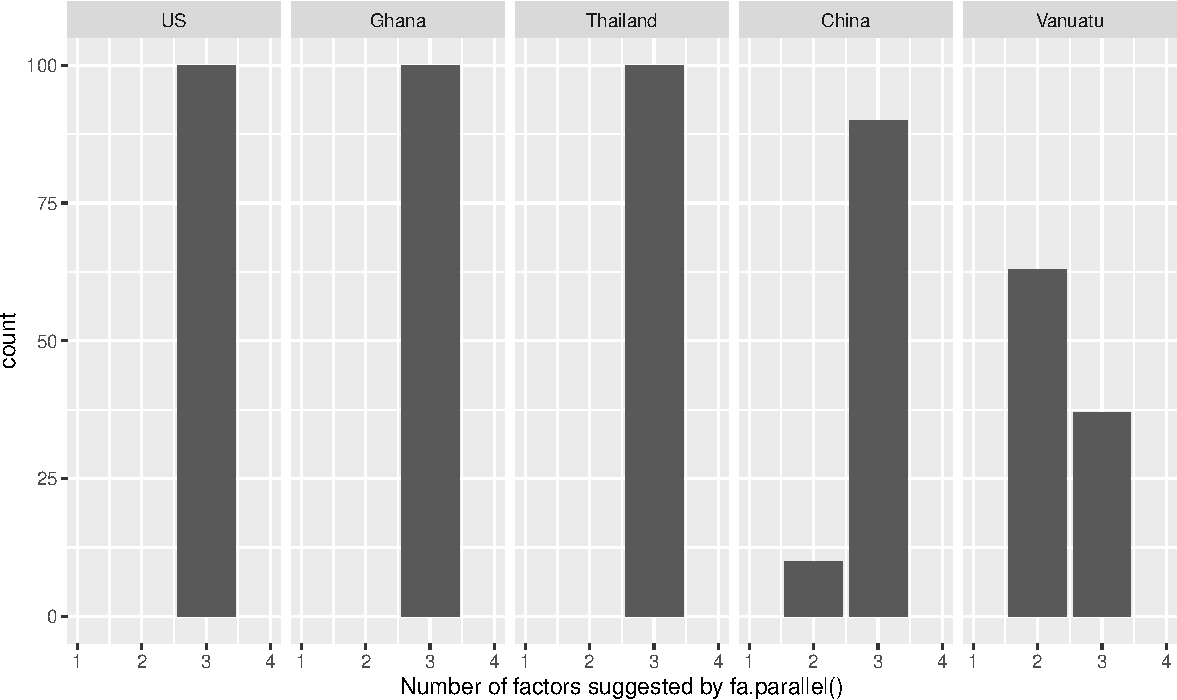
\includegraphics{Script_Re_Weisman_2021_Group1_2024_files/figure-latex/parallel dist adults-1.pdf}

\hypertarget{exploratory-factor-analysis-factor-loadings}{%
\subsubsection{Exploratory factor analysis: Factor loadings}\label{exploratory-factor-analysis-factor-loadings}}

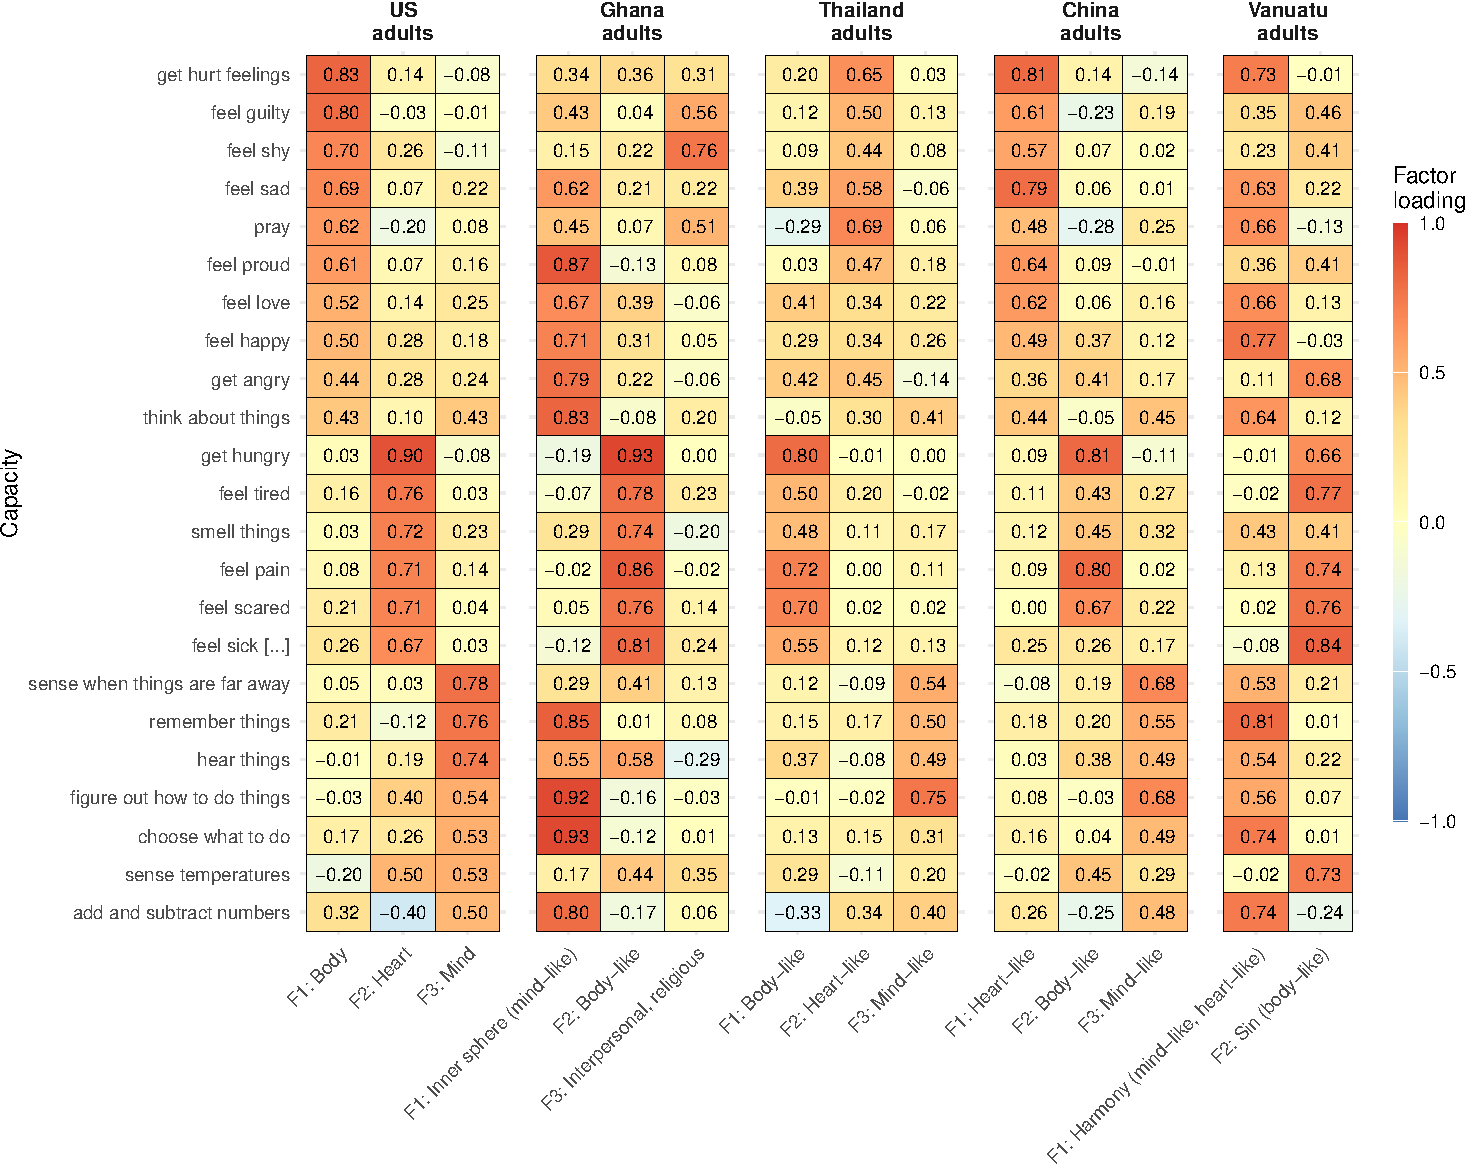
\includegraphics{Script_Re_Weisman_2021_Group1_2024_files/figure-latex/heatmap adults-1.pdf}

\hypertarget{congruence}{%
\subsubsection{Congruence}\label{congruence}}

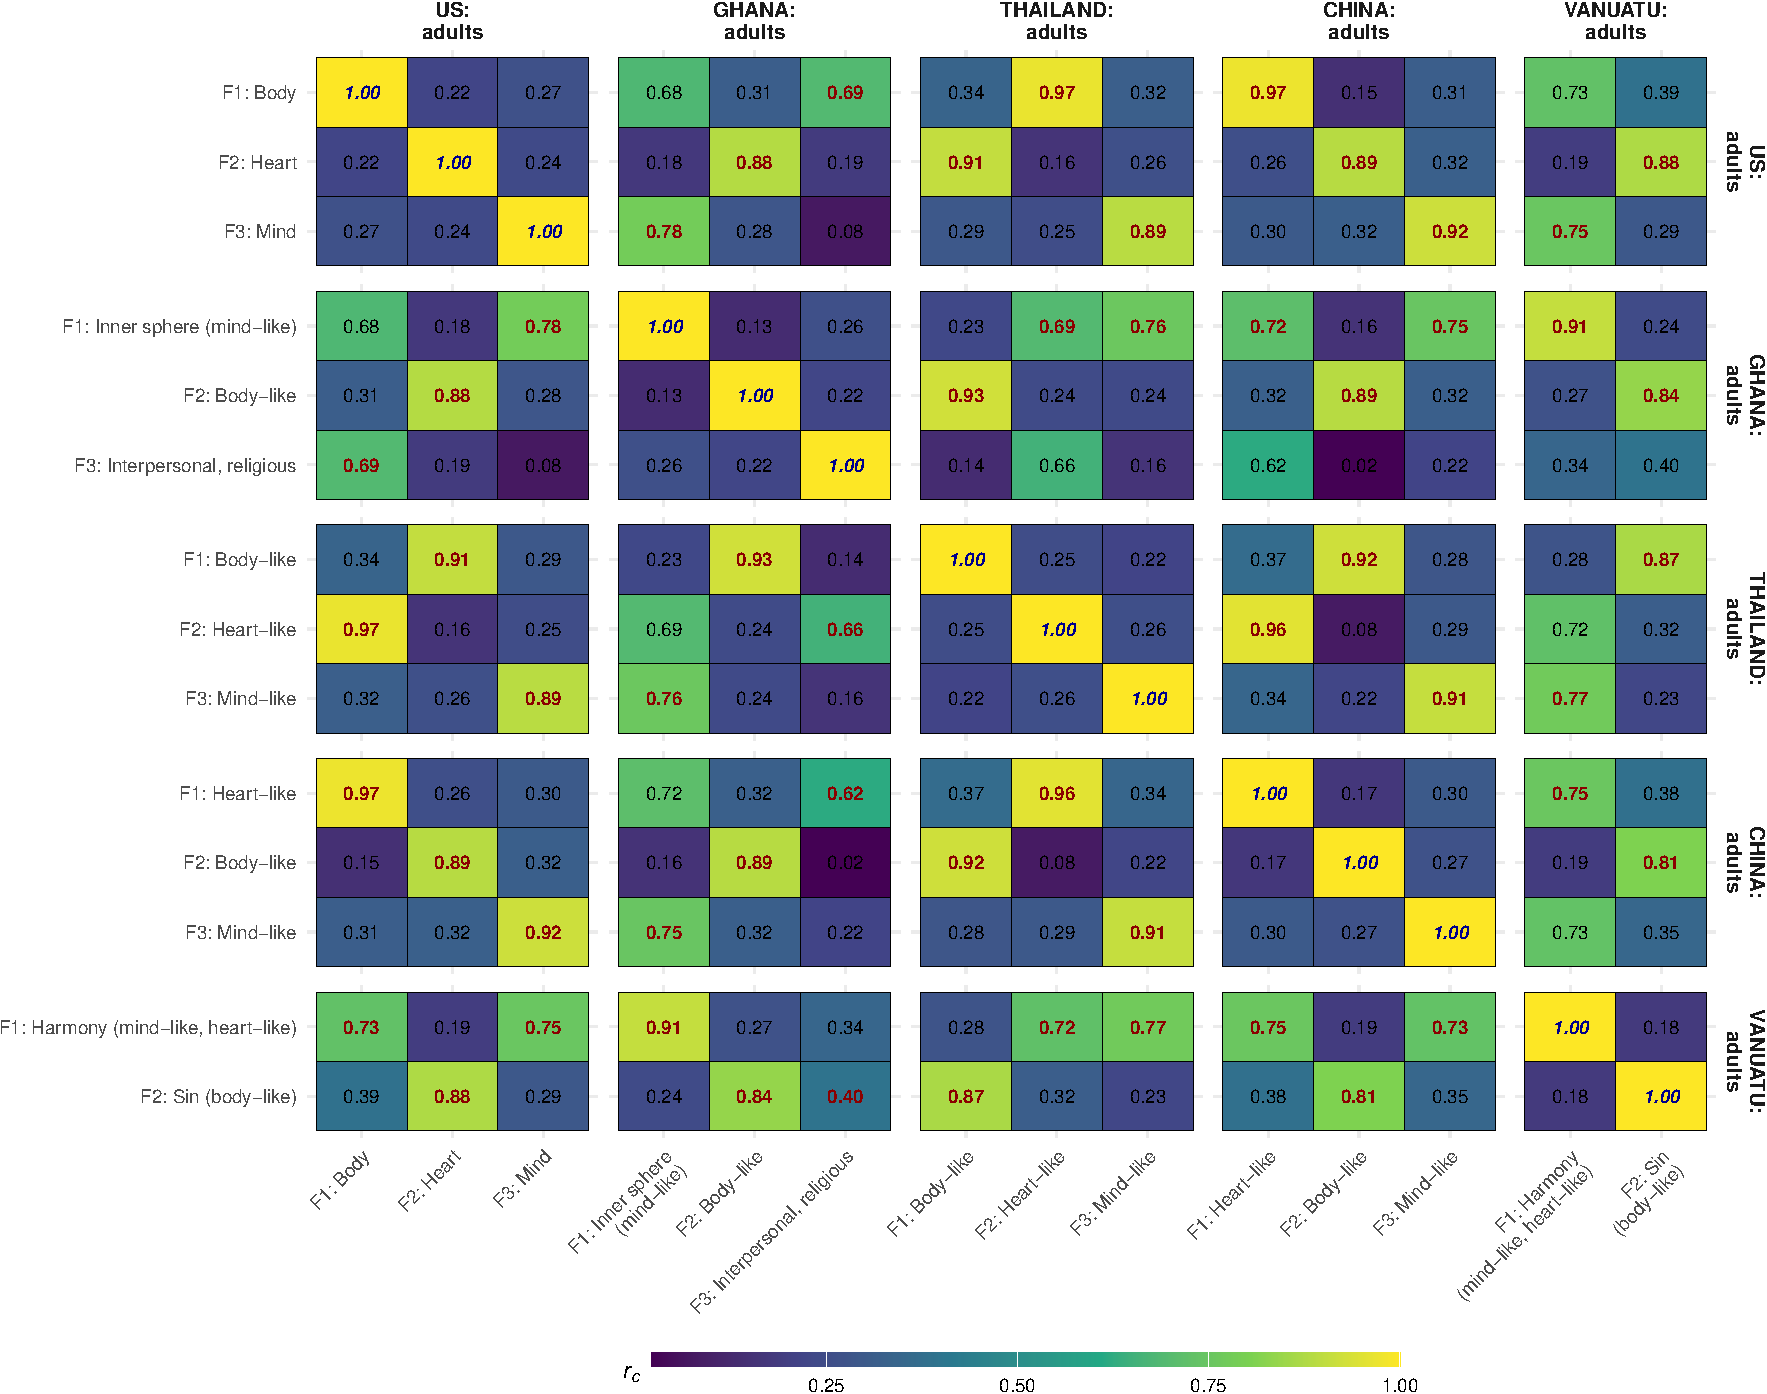
\includegraphics{Script_Re_Weisman_2021_Group1_2024_files/figure-latex/cong all pairs adults-1.pdf}

\hypertarget{bootstrapped-congruence}{%
\subsubsection{Bootstrapped congruence}\label{bootstrapped-congruence}}

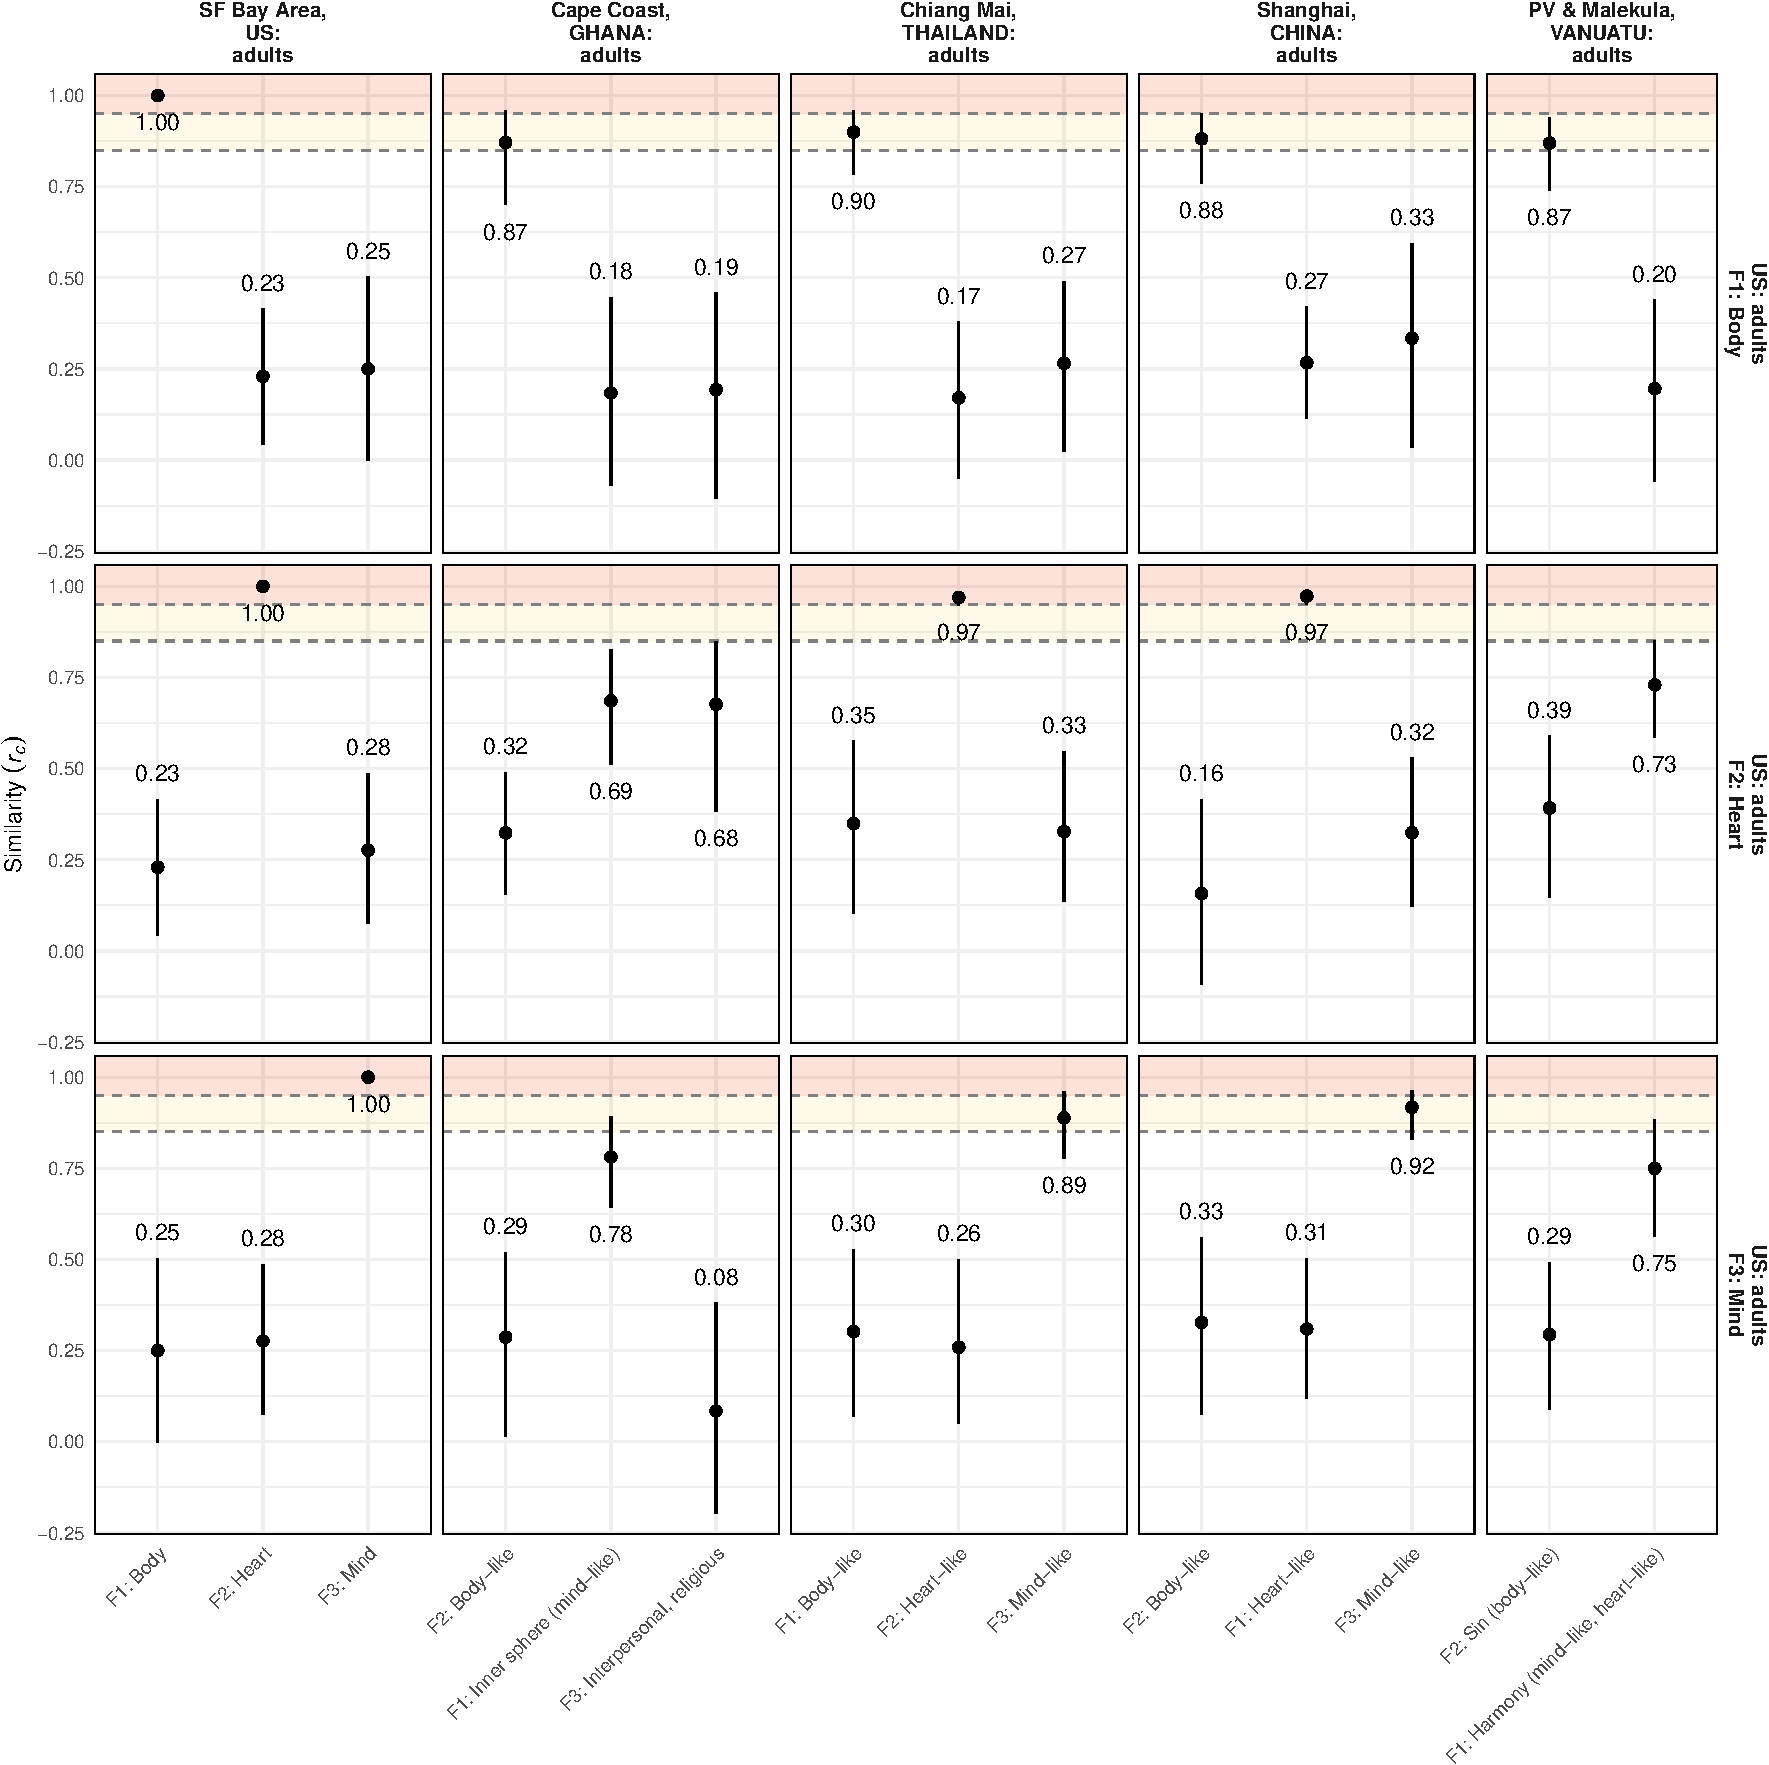
\includegraphics{Script_Re_Weisman_2021_Group1_2024_files/figure-latex/cong cis us base adults-1.pdf}

\hypertarget{figure-s2}{%
\subsubsection{FIGURE S2}\label{figure-s2}}

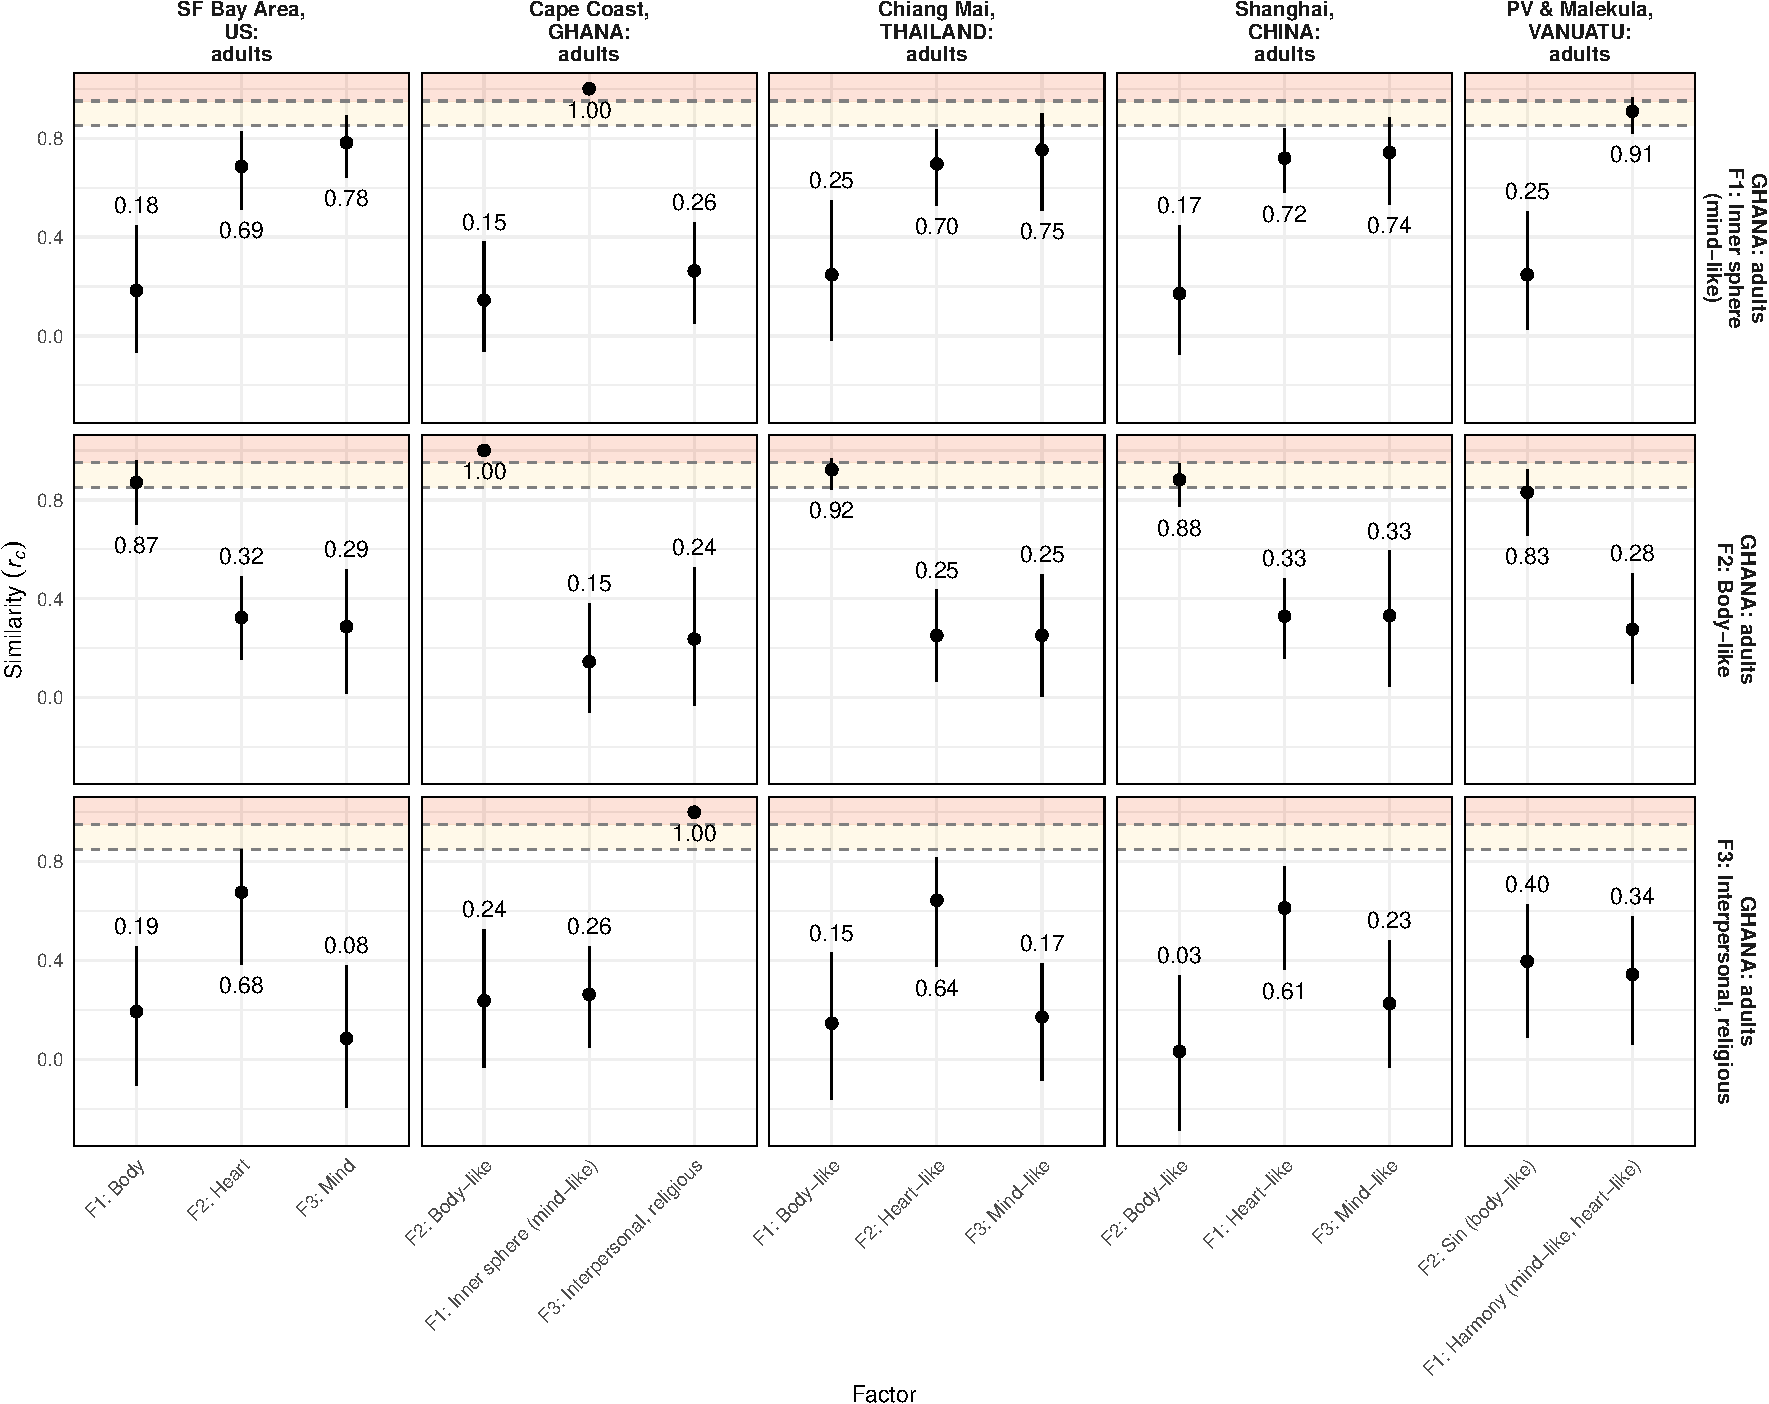
\includegraphics{Script_Re_Weisman_2021_Group1_2024_files/figure-latex/cong cis gh base adults-1.pdf}

\hypertarget{figure-s3}{%
\subsubsection{FIGURE S3}\label{figure-s3}}

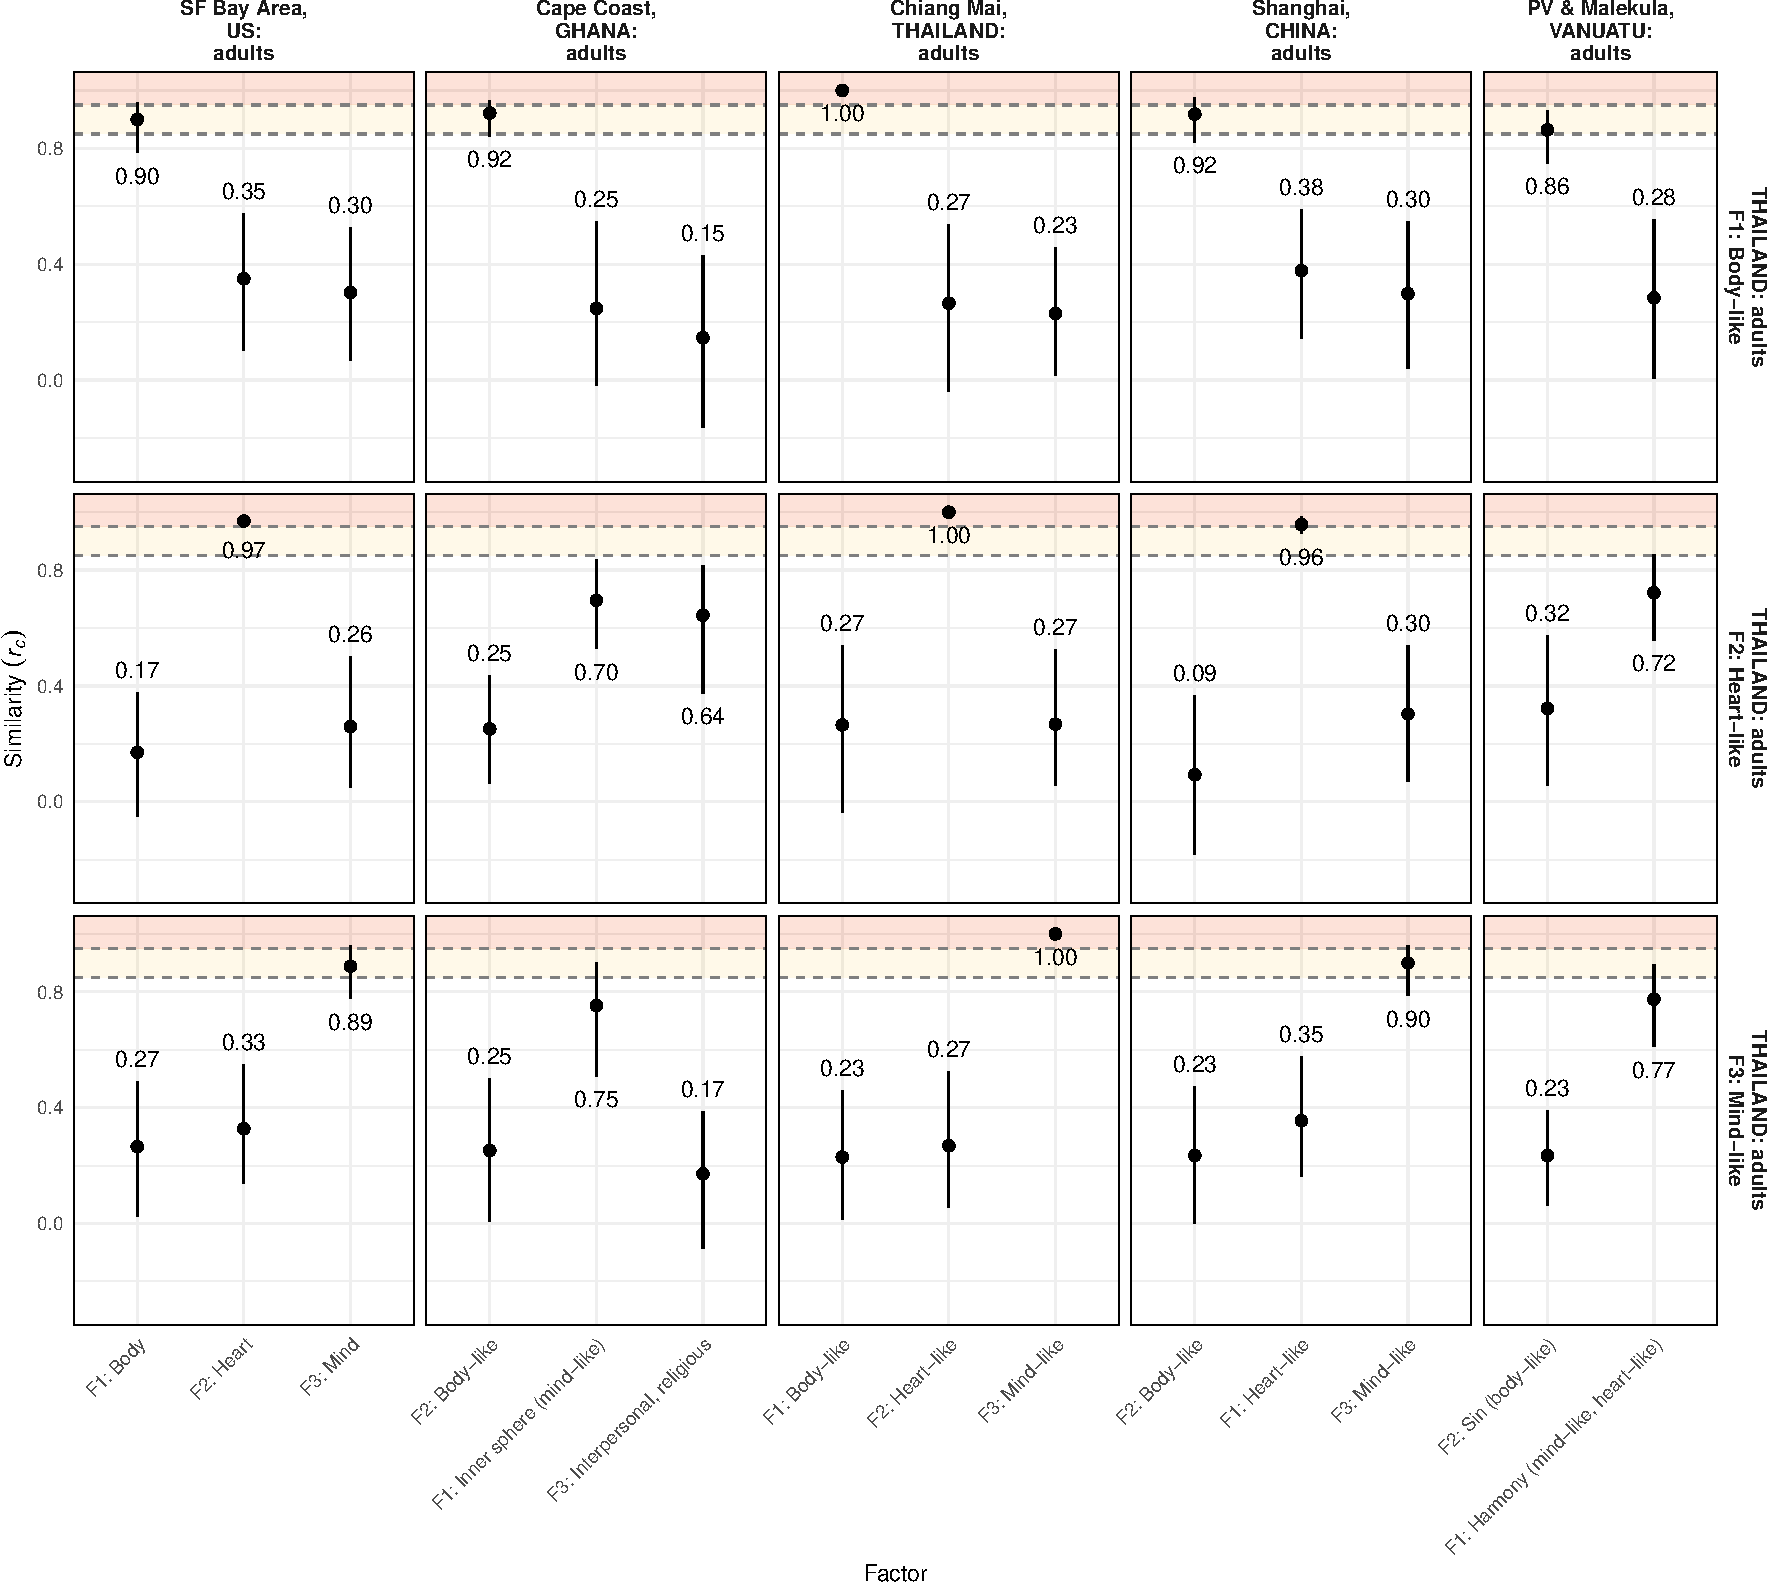
\includegraphics{Script_Re_Weisman_2021_Group1_2024_files/figure-latex/cong cis th base adults-1.pdf}

\hypertarget{figure-s4}{%
\subsubsection{FIGURE S4}\label{figure-s4}}

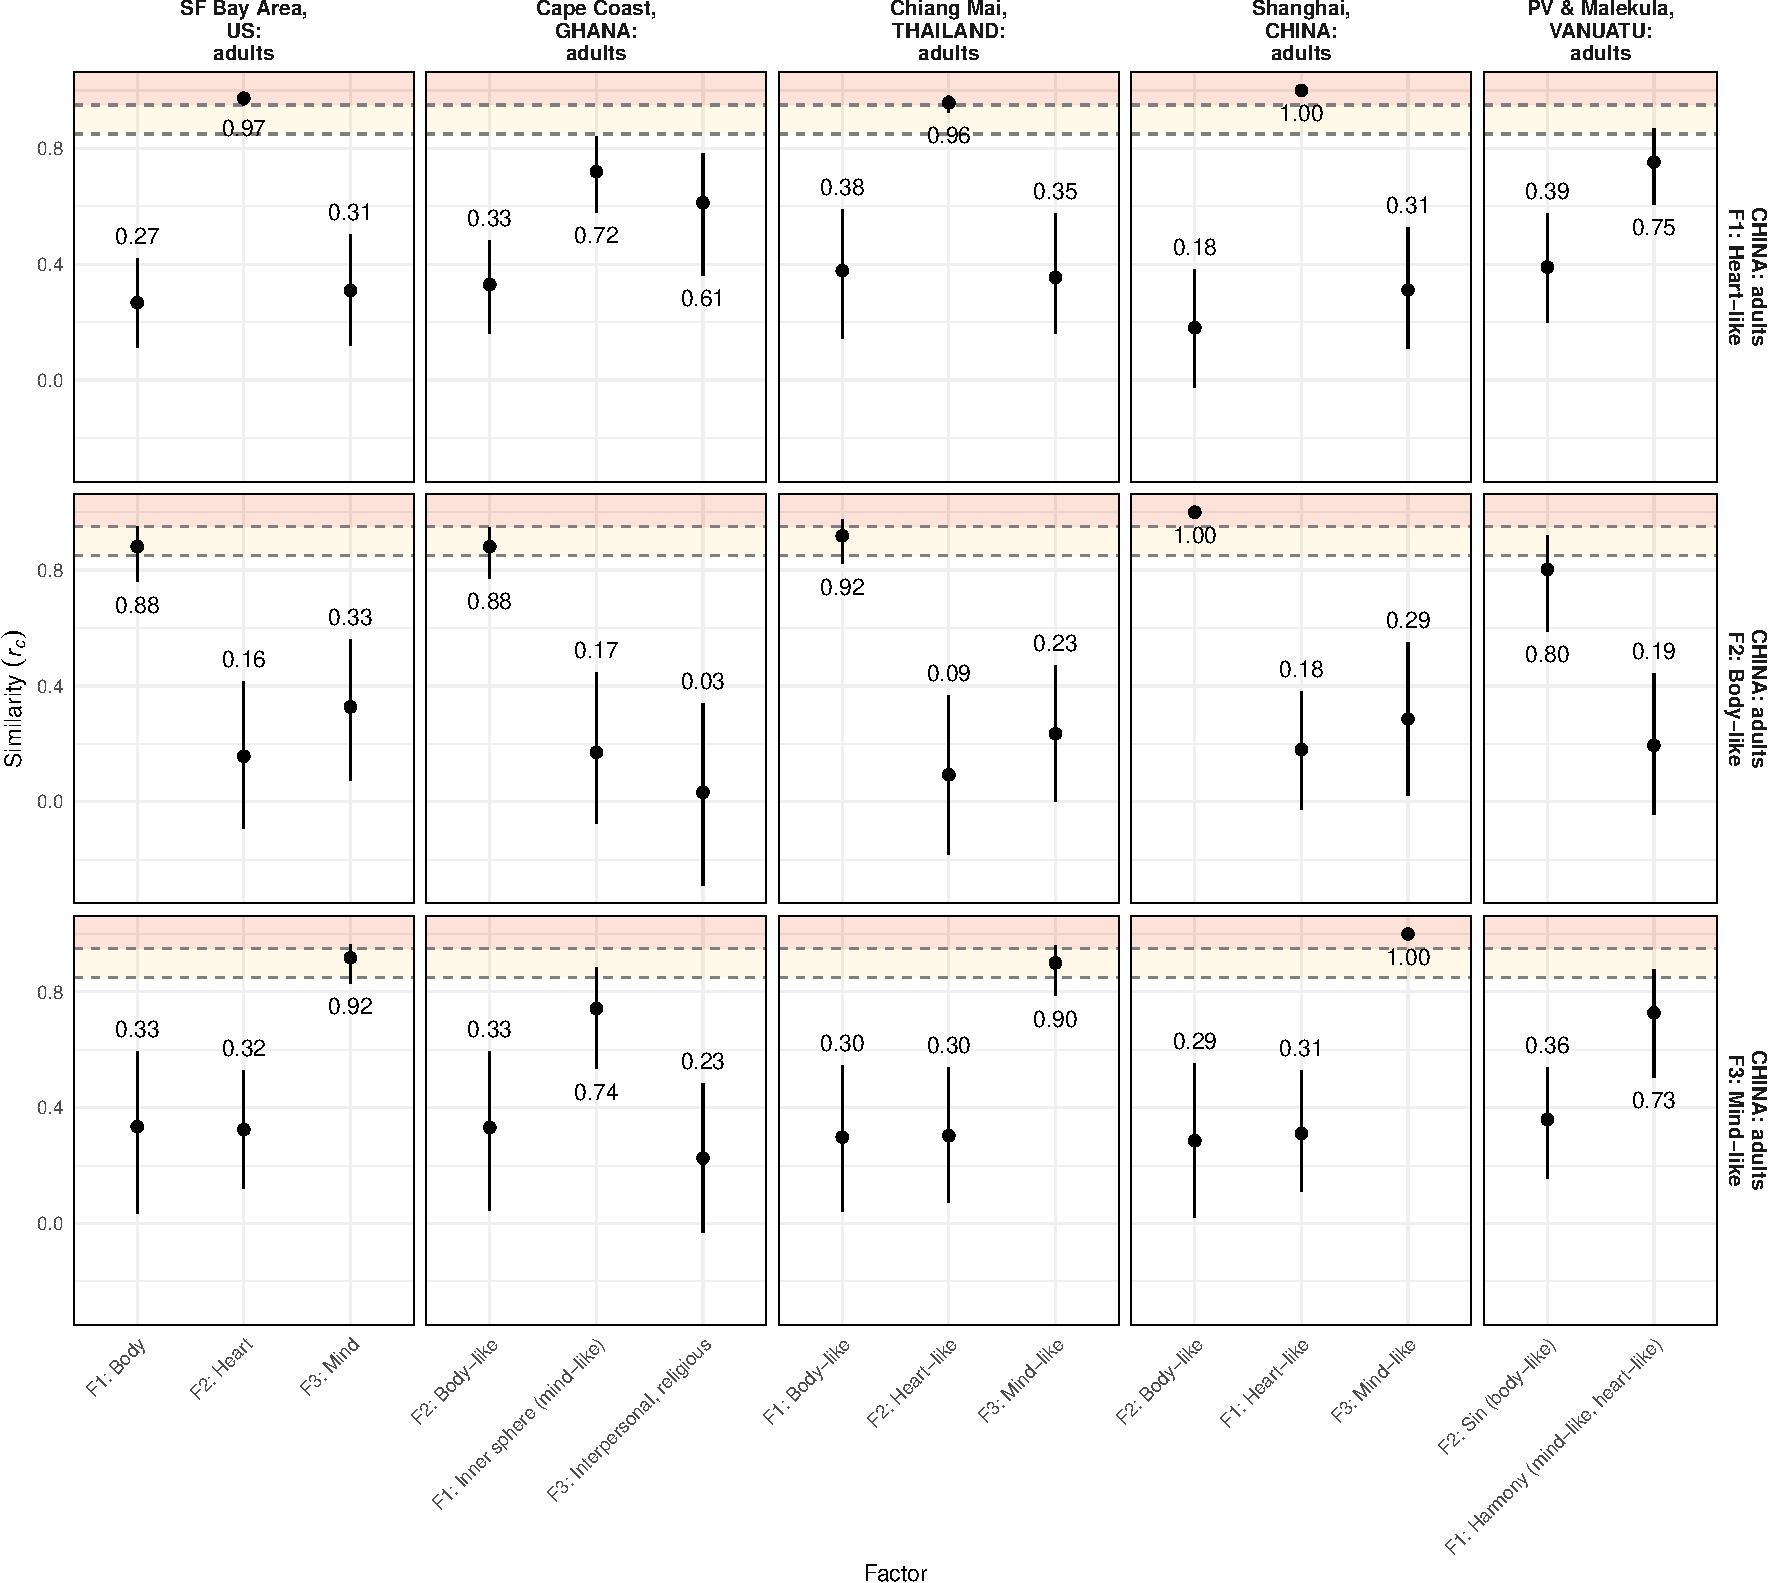
\includegraphics{Script_Re_Weisman_2021_Group1_2024_files/figure-latex/cong cis ch base adults-1.pdf}

\hypertarget{figure-s5}{%
\subsubsection{FIGURE S5}\label{figure-s5}}

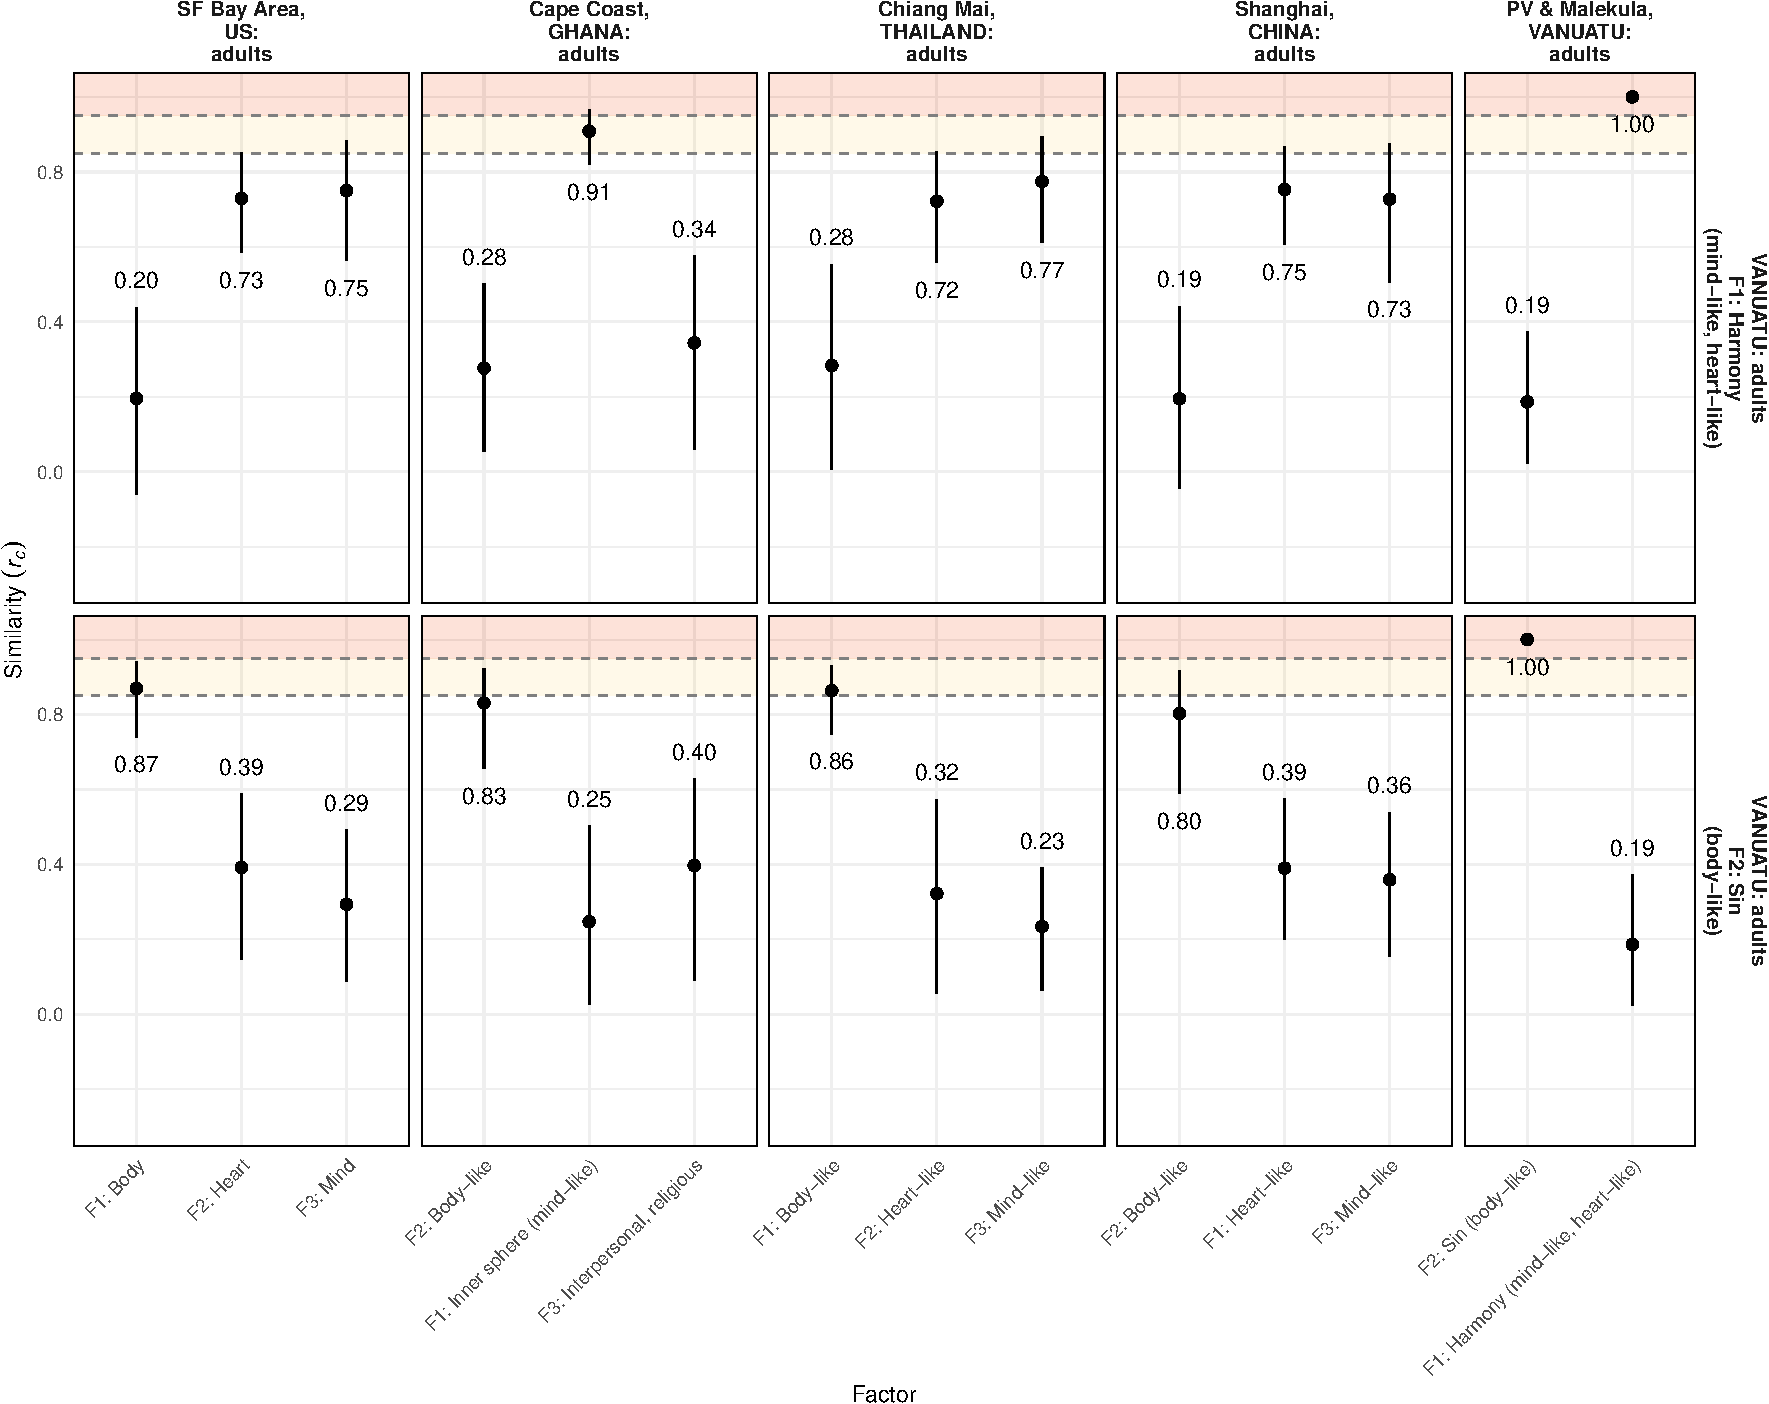
\includegraphics{Script_Re_Weisman_2021_Group1_2024_files/figure-latex/cong cis vt base adults-1.pdf}

\begin{verbatim}
## # A tibble: 4 x 15
##   factor_A  factor_B  mean ci_lower ci_upper age_group_A country_A factor_name_A
##   <chr>     <chr>    <dbl>    <dbl>    <dbl> <chr>       <fct>     <chr>        
## 1 chADULTS~ usADULT~ 0.881    0.760    0.950 adults      China     Ch. adults F~
## 2 ghADULTS~ usADULT~ 0.871    0.700    0.959 adults      Ghana     Gh. adults F~
## 3 thADULTS~ usADULT~ 0.900    0.785    0.959 adults      Thailand  Th. adults F~
## 4 vtADULTS~ usADULT~ 0.870    0.739    0.941 adults      Vanuatu   Va. adults F~
## # i 7 more variables: factor_descript_A <chr>, factor_labdescript_A <chr>,
## #   age_group_B <chr>, country_B <fct>, factor_name_B <chr>,
## #   factor_descript_B <chr>, factor_labdescript_B <chr>
\end{verbatim}

\begin{verbatim}
## # A tibble: 4 x 15
##   factor_A  factor_B  mean ci_lower ci_upper age_group_A country_A factor_name_A
##   <chr>     <chr>    <dbl>    <dbl>    <dbl> <chr>       <fct>     <chr>        
## 1 chADULTS~ usADULT~ 0.327   0.0743    0.562 adults      China     Ch. adults F~
## 2 ghADULTS~ usADULT~ 0.287   0.0151    0.520 adults      Ghana     Gh. adults F~
## 3 thADULTS~ usADULT~ 0.302   0.0686    0.527 adults      Thailand  Th. adults F~
## 4 vtADULTS~ usADULT~ 0.294   0.0876    0.492 adults      Vanuatu   Va. adults F~
## # i 7 more variables: factor_descript_A <chr>, factor_labdescript_A <chr>,
## #   age_group_B <chr>, country_B <fct>, factor_name_B <chr>,
## #   factor_descript_B <chr>, factor_labdescript_B <chr>
\end{verbatim}

\begin{verbatim}
## # A tibble: 4 x 15
##   factor_A  factor_B  mean ci_lower ci_upper age_group_A country_A factor_name_A
##   <chr>     <chr>    <dbl>    <dbl>    <dbl> <chr>       <fct>     <chr>        
## 1 chADULTS~ usADULT~ 0.917    0.830    0.962 adults      China     Ch. adults F~
## 2 ghADULTS~ usADULT~ 0.781    0.642    0.892 adults      Ghana     Gh. adults F~
## 3 thADULTS~ usADULT~ 0.889    0.777    0.960 adults      Thailand  Th. adults F~
## 4 vtADULTS~ usADULT~ 0.750    0.563    0.885 adults      Vanuatu   Va. adults F~
## # i 7 more variables: factor_descript_A <chr>, factor_labdescript_A <chr>,
## #   age_group_B <chr>, country_B <fct>, factor_name_B <chr>,
## #   factor_descript_B <chr>, factor_labdescript_B <chr>
\end{verbatim}

\begin{verbatim}
## # A tibble: 4 x 15
##   factor_A  factor_B  mean ci_lower ci_upper age_group_A country_A factor_name_A
##   <chr>     <chr>    <dbl>    <dbl>    <dbl> <chr>       <fct>     <chr>        
## 1 chADULTS~ usADULT~ 0.334   0.0356    0.595 adults      China     Ch. adults F~
## 2 ghADULTS~ usADULT~ 0.184  -0.0690    0.447 adults      Ghana     Gh. adults F~
## 3 thADULTS~ usADULT~ 0.265   0.0244    0.490 adults      Thailand  Th. adults F~
## 4 vtADULTS~ usADULT~ 0.196  -0.0597    0.439 adults      Vanuatu   Va. adults F~
## # i 7 more variables: factor_descript_A <chr>, factor_labdescript_A <chr>,
## #   age_group_B <chr>, country_B <fct>, factor_name_B <chr>,
## #   factor_descript_B <chr>, factor_labdescript_B <chr>
\end{verbatim}

\begin{verbatim}
## # A tibble: 2 x 15
##   factor_A  factor_B  mean ci_lower ci_upper age_group_A country_A factor_name_A
##   <chr>     <chr>    <dbl>    <dbl>    <dbl> <chr>       <fct>     <chr>        
## 1 chADULTS~ usADULT~ 0.973    0.949    0.987 adults      China     Ch. adults F~
## 2 thADULTS~ usADULT~ 0.969    0.947    0.986 adults      Thailand  Th. adults F~
## # i 7 more variables: factor_descript_A <chr>, factor_labdescript_A <chr>,
## #   age_group_B <chr>, country_B <fct>, factor_name_B <chr>,
## #   factor_descript_B <chr>, factor_labdescript_B <chr>
\end{verbatim}

\begin{verbatim}
## # A tibble: 4 x 15
##   factor_A  factor_B  mean ci_lower ci_upper age_group_A country_A factor_name_A
##   <chr>     <chr>    <dbl>    <dbl>    <dbl> <chr>       <fct>     <chr>        
## 1 chADULTS~ usADULT~ 0.157  -0.0930    0.416 adults      China     Ch. adults F~
## 2 chADULTS~ usADULT~ 0.324   0.122     0.530 adults      China     Ch. adults F~
## 3 thADULTS~ usADULT~ 0.349   0.103     0.576 adults      Thailand  Th. adults F~
## 4 thADULTS~ usADULT~ 0.327   0.137     0.548 adults      Thailand  Th. adults F~
## # i 7 more variables: factor_descript_A <chr>, factor_labdescript_A <chr>,
## #   age_group_B <chr>, country_B <fct>, factor_name_B <chr>,
## #   factor_descript_B <chr>, factor_labdescript_B <chr>
\end{verbatim}

\hypertarget{primary-analysis-children}{%
\subsection{3.3 Primary Analysis (Children)}\label{primary-analysis-children}}

\hypertarget{samples-1}{%
\subsubsection{Samples}\label{samples-1}}

\begin{tabular}{l|r}
\hline
country & n\\
\hline
US & 117\\
\hline
Ghana & 150\\
\hline
Thailand & 152\\
\hline
China & 131\\
\hline
Vanuatu & 143\\
\hline
Total & 693\\
\hline
\end{tabular}

\hypertarget{scale-use-1}{%
\subsubsection{Scale use}\label{scale-use-1}}

\begin{tabular}{l|l|l|l|l}
\hline
country & no & kind of & yes & missing data\\
\hline
US & 42.14\% & 16.09\% & 40.88\% & 0.89\%\\
\hline
Ghana & 54.12\% & 1.48\% & 44.09\% & 0.32\%\\
\hline
Thailand & 37.99\% & 25.86\% & 35.90\% & 0.26\%\\
\hline
China & 35.01\% & 17.03\% & 47.00\% & 0.96\%\\
\hline
Vanuatu & 50.02\% & 3.89\% & 46.03\% & 0.06\%\\
\hline
\end{tabular}

\hypertarget{factor-retention-parallel-analysis-1}{%
\subsubsection{Factor retention: parallel analysis}\label{factor-retention-parallel-analysis-1}}

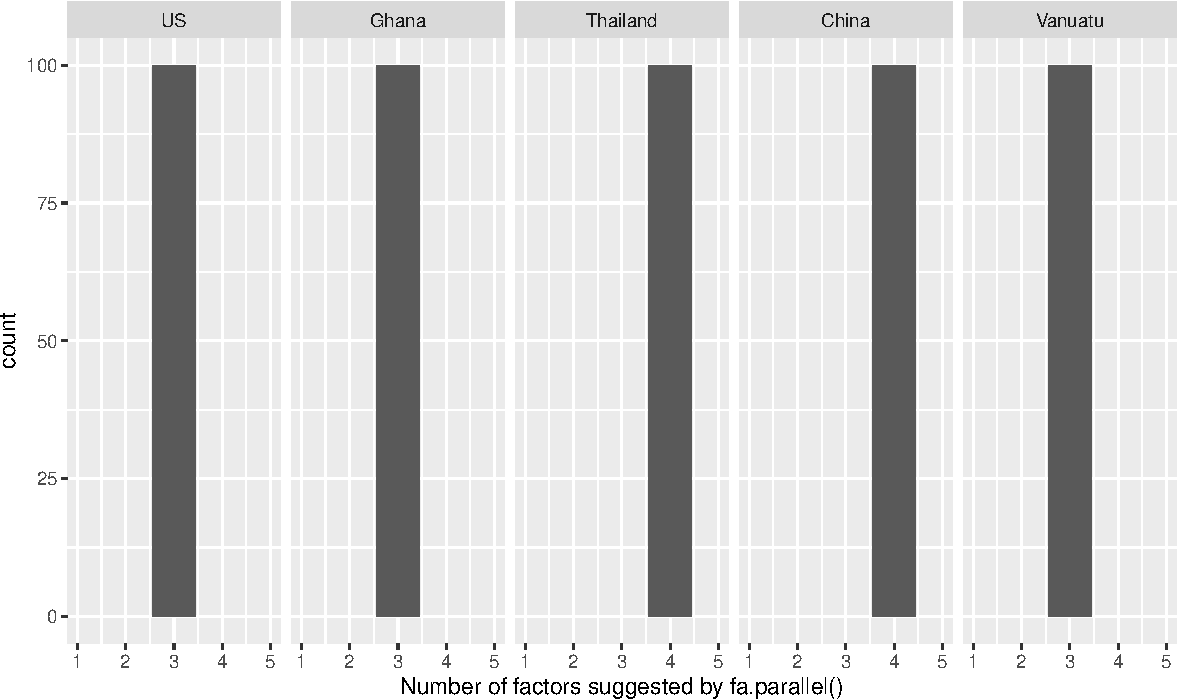
\includegraphics{Script_Re_Weisman_2021_Group1_2024_files/figure-latex/parallel dist children-1.pdf}

\hypertarget{exploratory-factor-analysis-factor-loadings-1}{%
\subsubsection{Exploratory factor analysis: Factor loadings}\label{exploratory-factor-analysis-factor-loadings-1}}

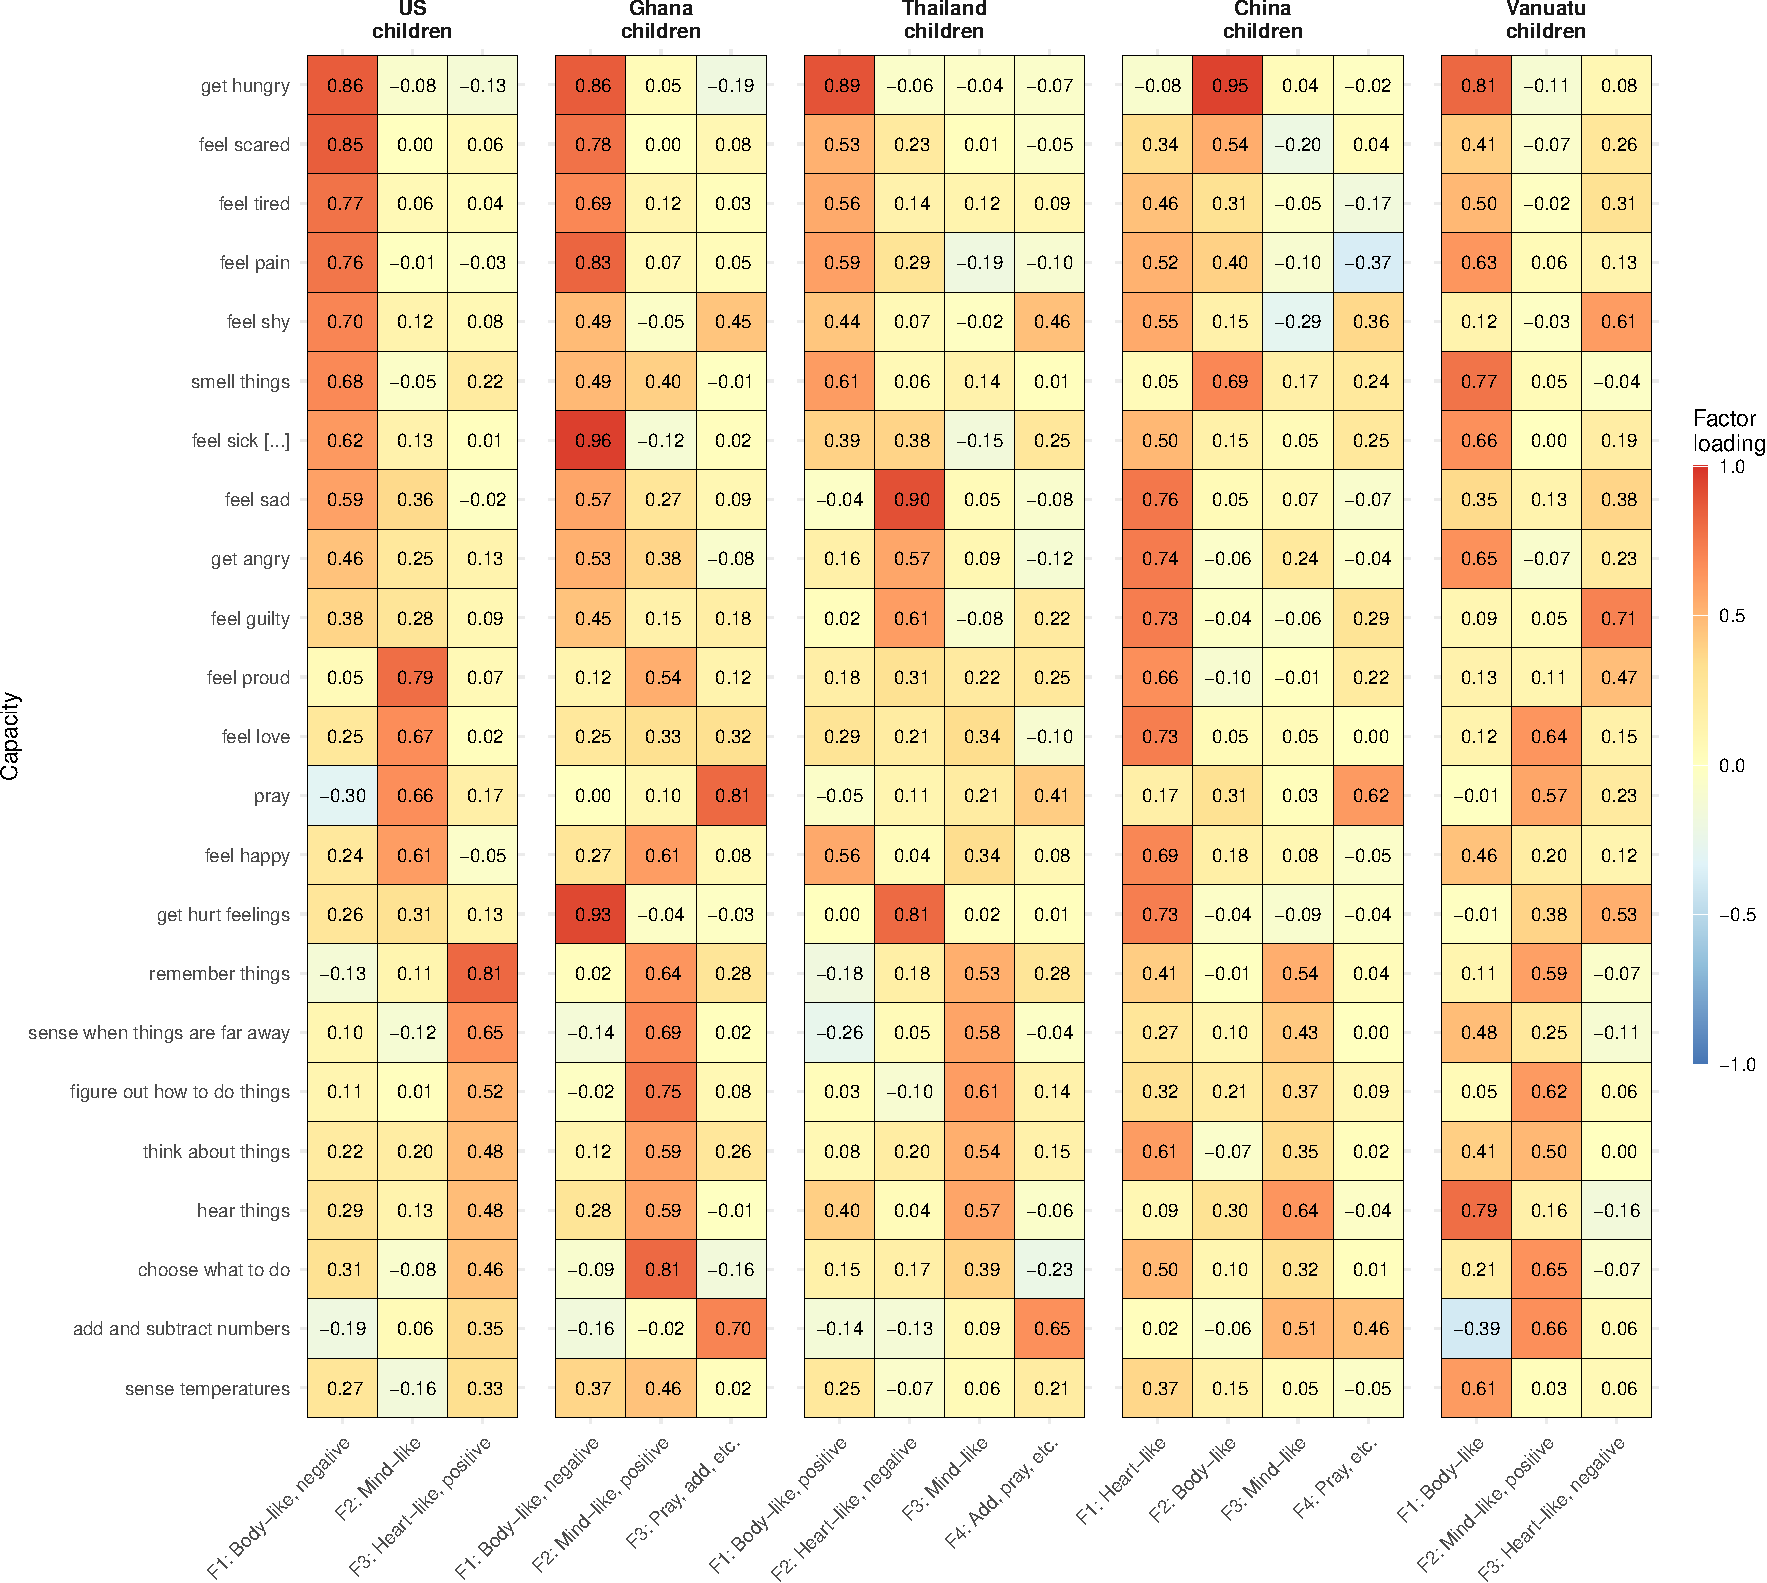
\includegraphics{Script_Re_Weisman_2021_Group1_2024_files/figure-latex/heatmap children-1.pdf}

\hypertarget{congruence-bootstrapped-congruence}{%
\subsection{Congruence: Bootstrapped congruence}\label{congruence-bootstrapped-congruence}}

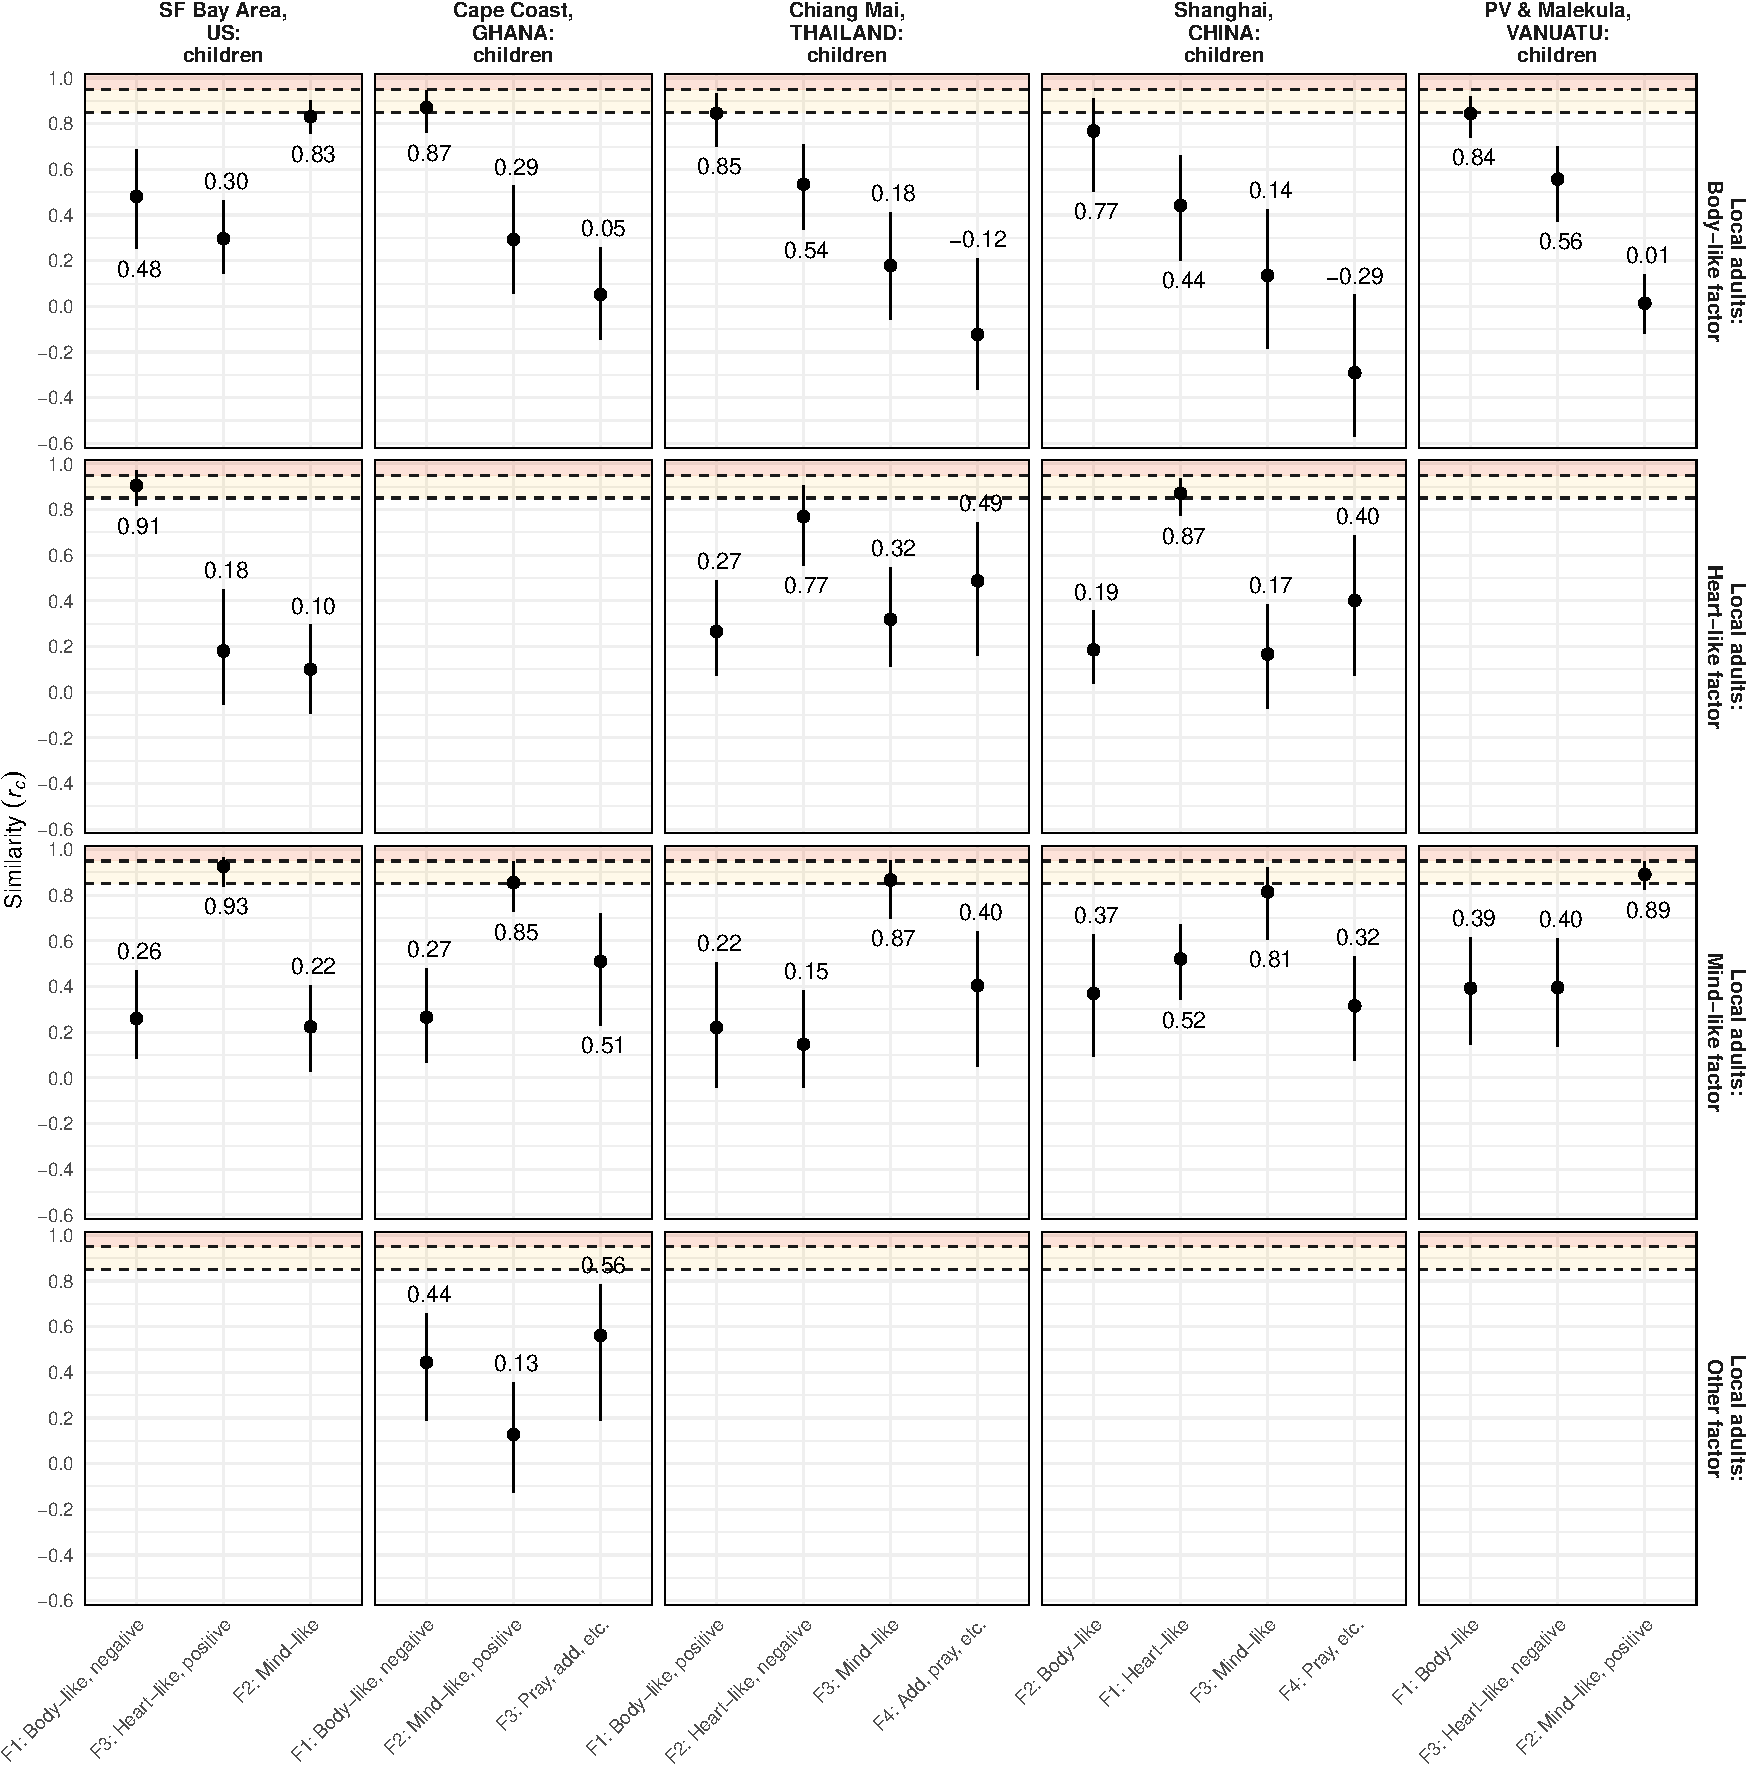
\includegraphics{Script_Re_Weisman_2021_Group1_2024_files/figure-latex/cong cis children b-1.pdf}

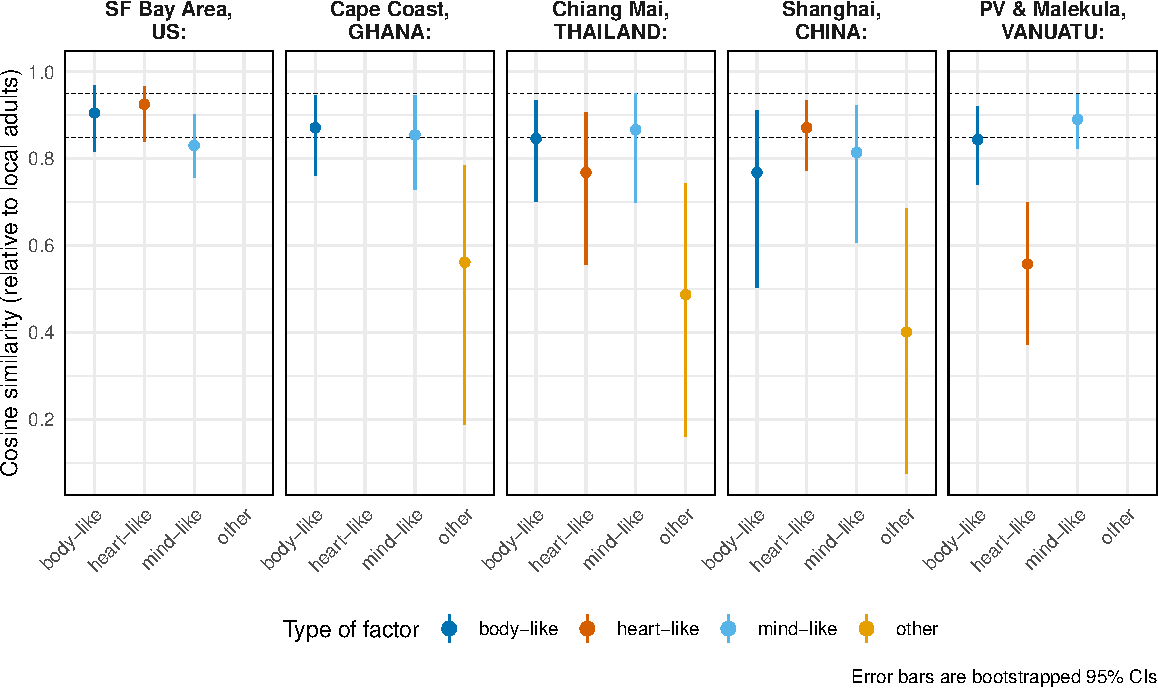
\includegraphics{Script_Re_Weisman_2021_Group1_2024_files/figure-latex/alt fig 4-1.pdf}

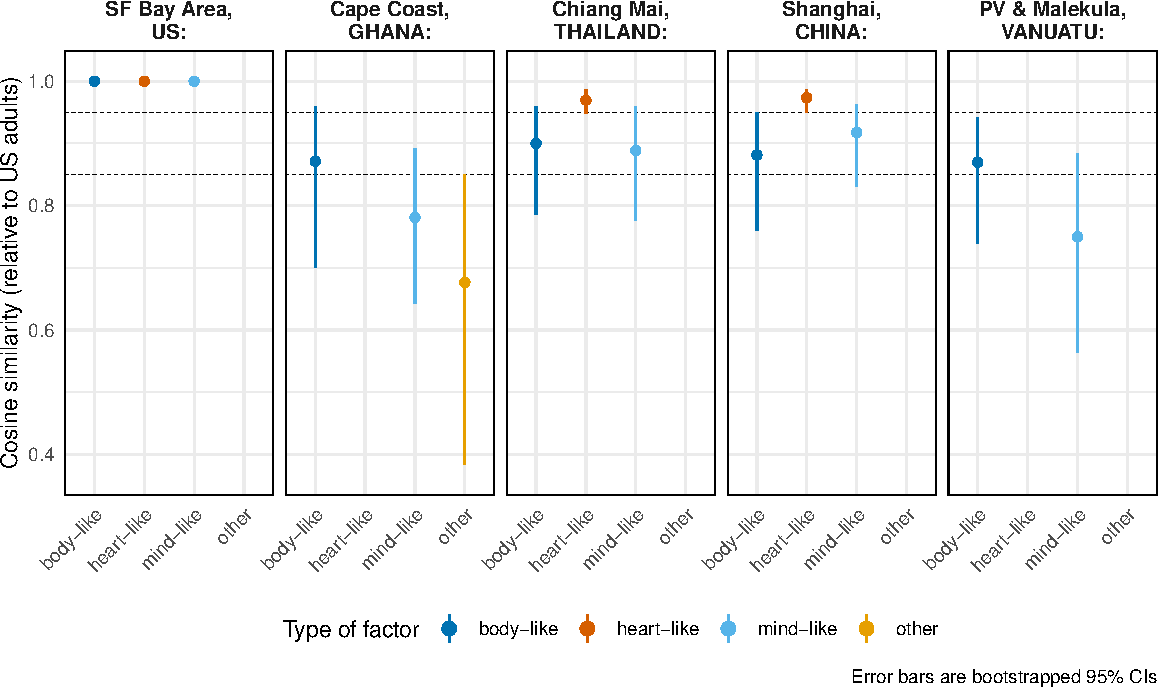
\includegraphics{Script_Re_Weisman_2021_Group1_2024_files/figure-latex/alt fig 3-1.pdf}

\begin{verbatim}
## # A tibble: 5 x 17
##   factor_A  factor_B  mean ci_lower ci_upper age_group_A country_A factor_name_A
##   <chr>     <chr>    <dbl>    <dbl>    <dbl> <chr>       <fct>     <chr>        
## 1 chCHILDR~ chADULT~ 0.768    0.503    0.912 children    China     Ch. children~
## 2 ghCHILDR~ ghADULT~ 0.871    0.761    0.946 children    Ghana     Gh. children~
## 3 thCHILDR~ thADULT~ 0.846    0.701    0.934 children    Thailand  Th. children~
## 4 usCHILDR~ usADULT~ 0.482    0.252    0.687 children    US        US children ~
## 5 vtCHILDR~ vtADULT~ 0.844    0.741    0.921 children    Vanuatu   Va. children~
## # i 9 more variables: factor_descript_A <chr>, factor_labdescript_A <chr>,
## #   age_group_B <chr>, country_B <fct>, factor_name_B <chr>,
## #   factor_descript_B <chr>, factor_labdescript_B <chr>, factor_bhm_A <chr>,
## #   factor_bhm_B <chr>
\end{verbatim}

\begin{verbatim}
## # A tibble: 5 x 17
##   factor_A  factor_B  mean ci_lower ci_upper age_group_A country_A factor_name_A
##   <chr>     <chr>    <dbl>    <dbl>    <dbl> <chr>       <fct>     <chr>        
## 1 chCHILDR~ chADULT~ 0.370   0.0946    0.628 children    China     Ch. children~
## 2 ghCHILDR~ ghADULT~ 0.266   0.0680    0.480 children    Ghana     Gh. children~
## 3 thCHILDR~ thADULT~ 0.221  -0.0443    0.507 children    Thailand  Th. children~
## 4 usCHILDR~ usADULT~ 0.259   0.0863    0.469 children    US        US children ~
## 5 vtCHILDR~ vtADULT~ 0.393   0.145     0.613 children    Vanuatu   Va. children~
## # i 9 more variables: factor_descript_A <chr>, factor_labdescript_A <chr>,
## #   age_group_B <chr>, country_B <fct>, factor_name_B <chr>,
## #   factor_descript_B <chr>, factor_labdescript_B <chr>, factor_bhm_A <chr>,
## #   factor_bhm_B <chr>
\end{verbatim}

\begin{verbatim}
## # A tibble: 5 x 17
##   factor_A  factor_B  mean ci_lower ci_upper age_group_A country_A factor_name_A
##   <chr>     <chr>    <dbl>    <dbl>    <dbl> <chr>       <fct>     <chr>        
## 1 chCHILDR~ chADULT~ 0.814   0.608     0.922 children    China     Ch. children~
## 2 ghCHILDR~ ghADULT~ 0.855   0.728     0.946 children    Ghana     Gh. children~
## 3 thCHILDR~ thADULT~ 0.867   0.699     0.951 children    Thailand  Th. children~
## 4 usCHILDR~ usADULT~ 0.223   0.0275    0.406 children    US        US children ~
## 5 vtCHILDR~ vtADULT~ 0.890   0.823     0.948 children    Vanuatu   Va. children~
## # i 9 more variables: factor_descript_A <chr>, factor_labdescript_A <chr>,
## #   age_group_B <chr>, country_B <fct>, factor_name_B <chr>,
## #   factor_descript_B <chr>, factor_labdescript_B <chr>, factor_bhm_A <chr>,
## #   factor_bhm_B <chr>
\end{verbatim}

\begin{verbatim}
## # A tibble: 5 x 17
##   factor_A factor_B   mean ci_lower ci_upper age_group_A country_A factor_name_A
##   <chr>    <chr>     <dbl>    <dbl>    <dbl> <chr>       <fct>     <chr>        
## 1 chCHILD~ chADULT~ 0.136   -0.183     0.424 children    China     Ch. children~
## 2 ghCHILD~ ghADULT~ 0.294    0.0574    0.528 children    Ghana     Gh. children~
## 3 thCHILD~ thADULT~ 0.178   -0.0564    0.411 children    Thailand  Th. children~
## 4 usCHILD~ usADULT~ 0.830    0.756     0.902 children    US        US children ~
## 5 vtCHILD~ vtADULT~ 0.0137  -0.117     0.140 children    Vanuatu   Va. children~
## # i 9 more variables: factor_descript_A <chr>, factor_labdescript_A <chr>,
## #   age_group_B <chr>, country_B <fct>, factor_name_B <chr>,
## #   factor_descript_B <chr>, factor_labdescript_B <chr>, factor_bhm_A <chr>,
## #   factor_bhm_B <chr>
\end{verbatim}

\hypertarget{primary-analysis-all-samples}{%
\subsection{3.4 Primary Analysis (All Samples)}\label{primary-analysis-all-samples}}

\hypertarget{congruence-1}{%
\subsubsection{Congruence}\label{congruence-1}}

\hypertarget{figure-2}{%
\subsubsection{Figure 2}\label{figure-2}}

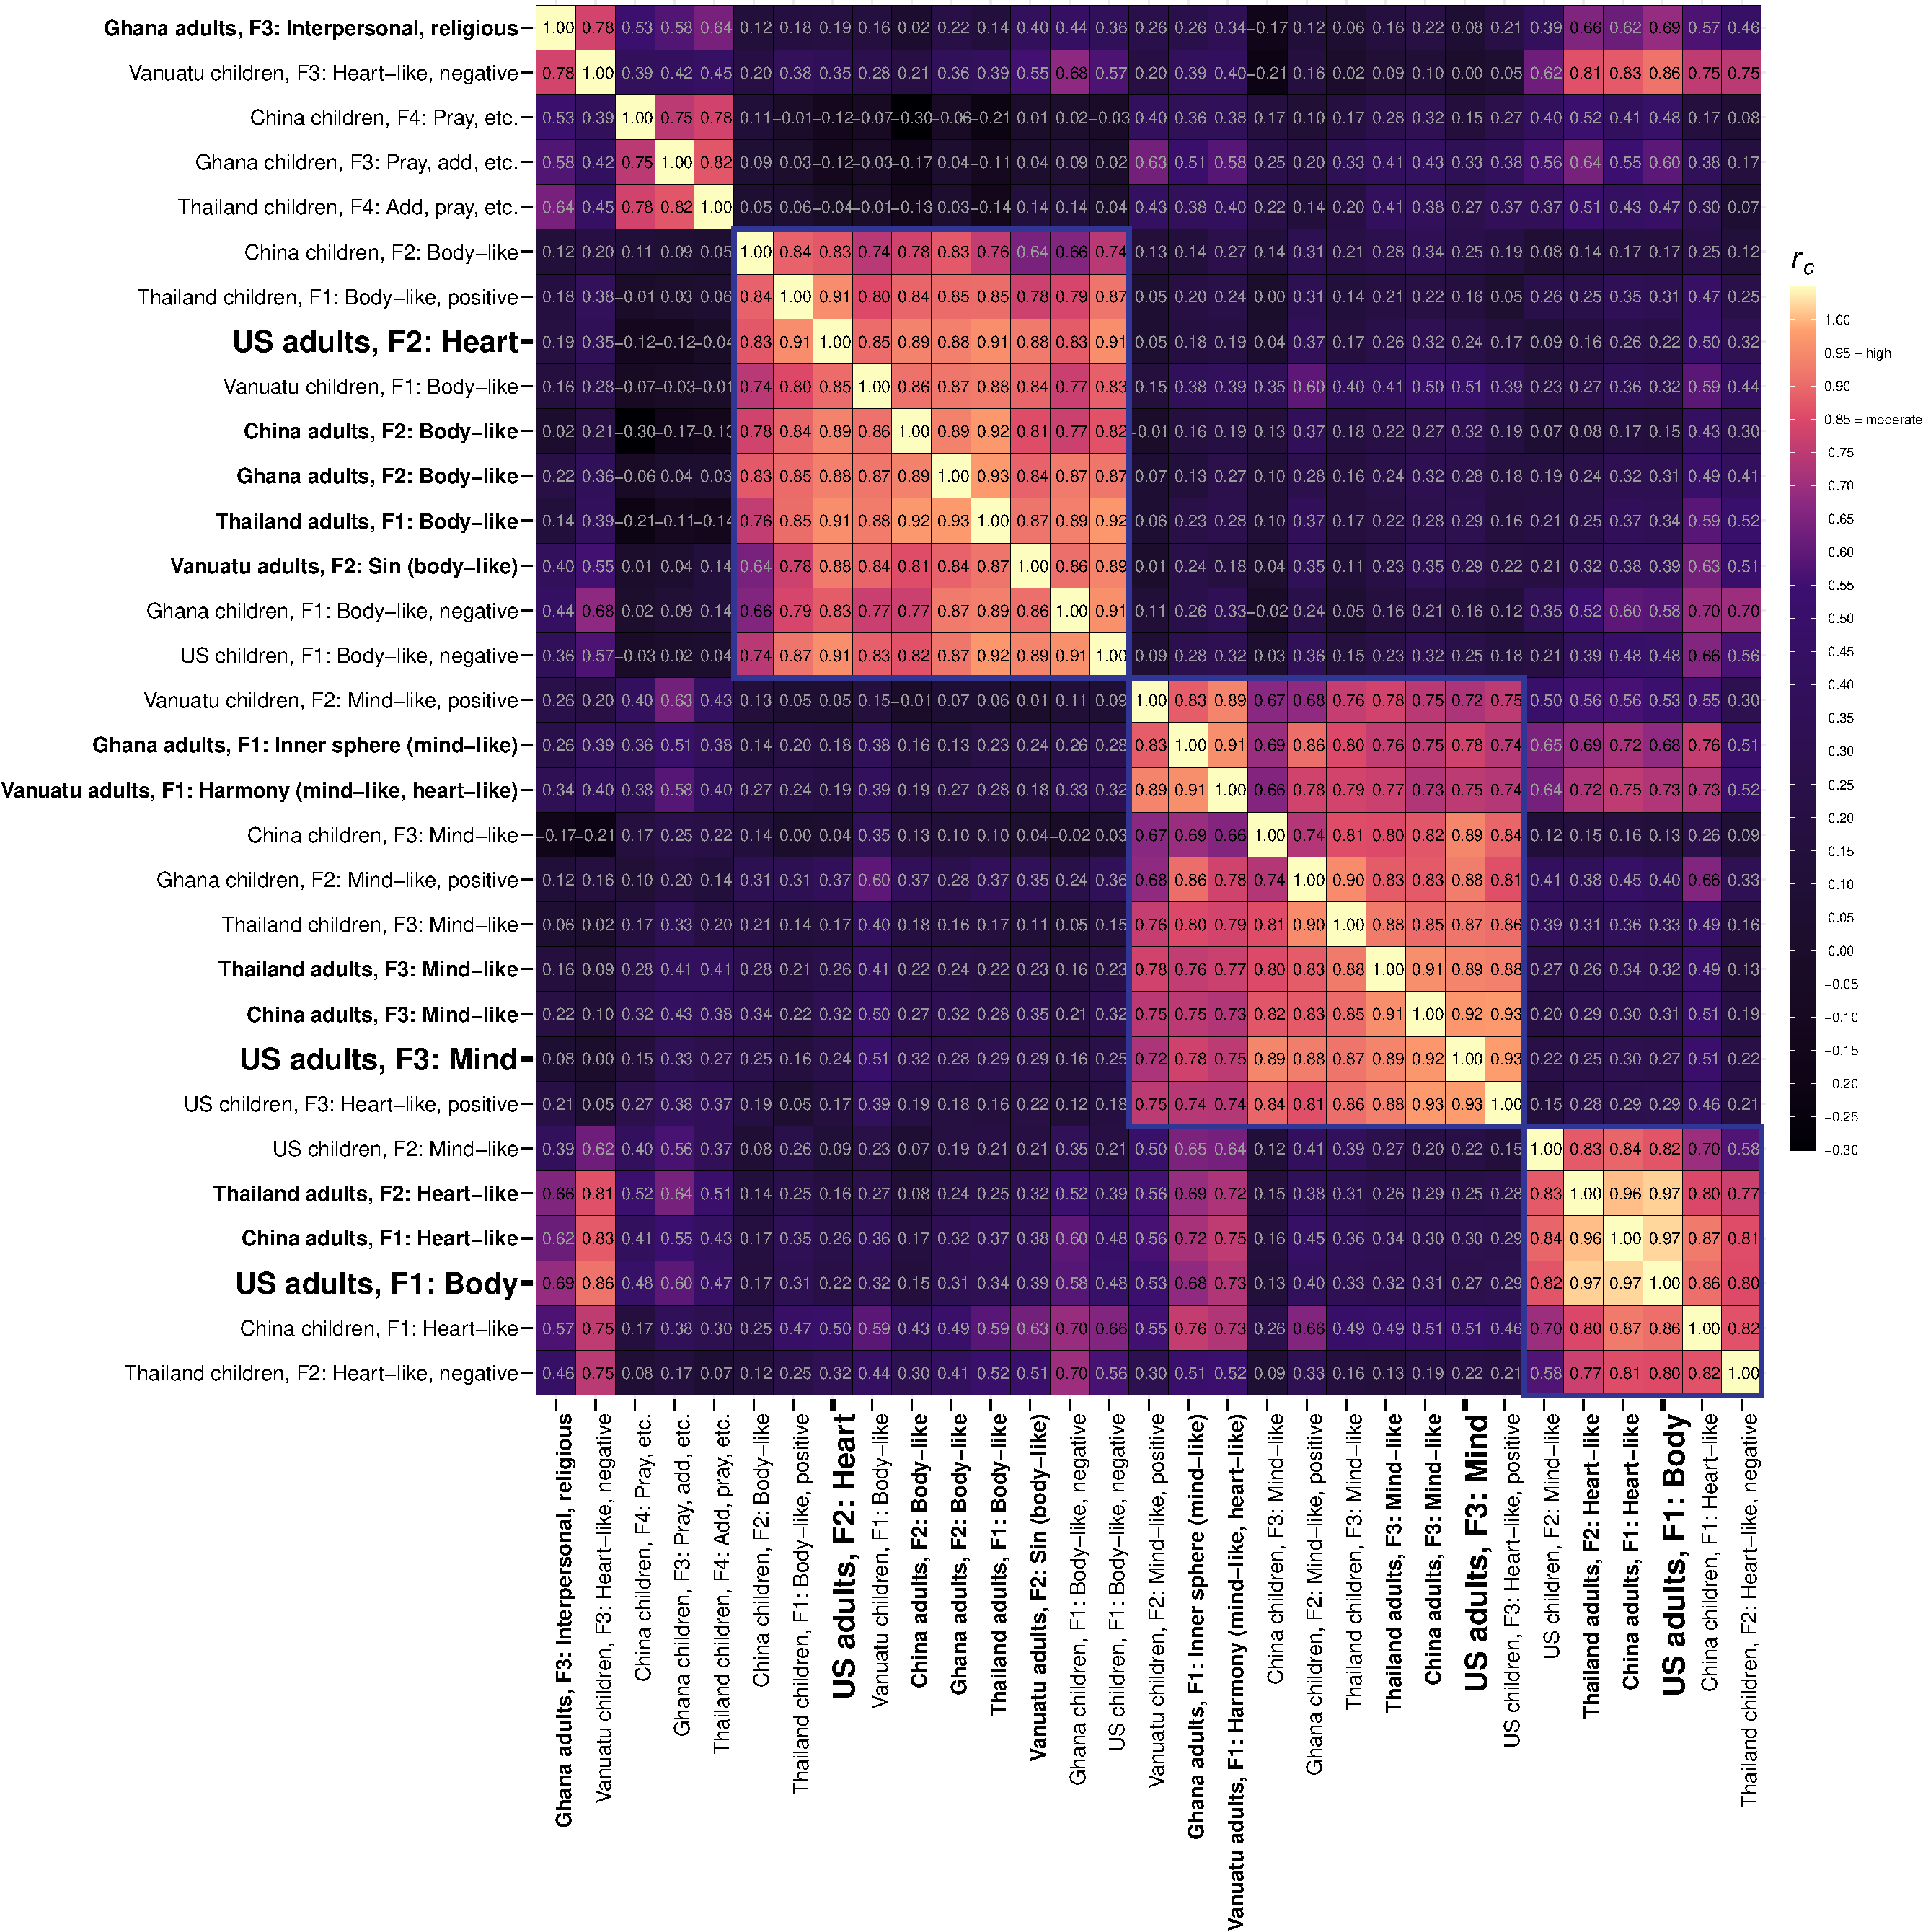
\includegraphics{Script_Re_Weisman_2021_Group1_2024_files/figure-latex/cong all pairs plot a-1.pdf}

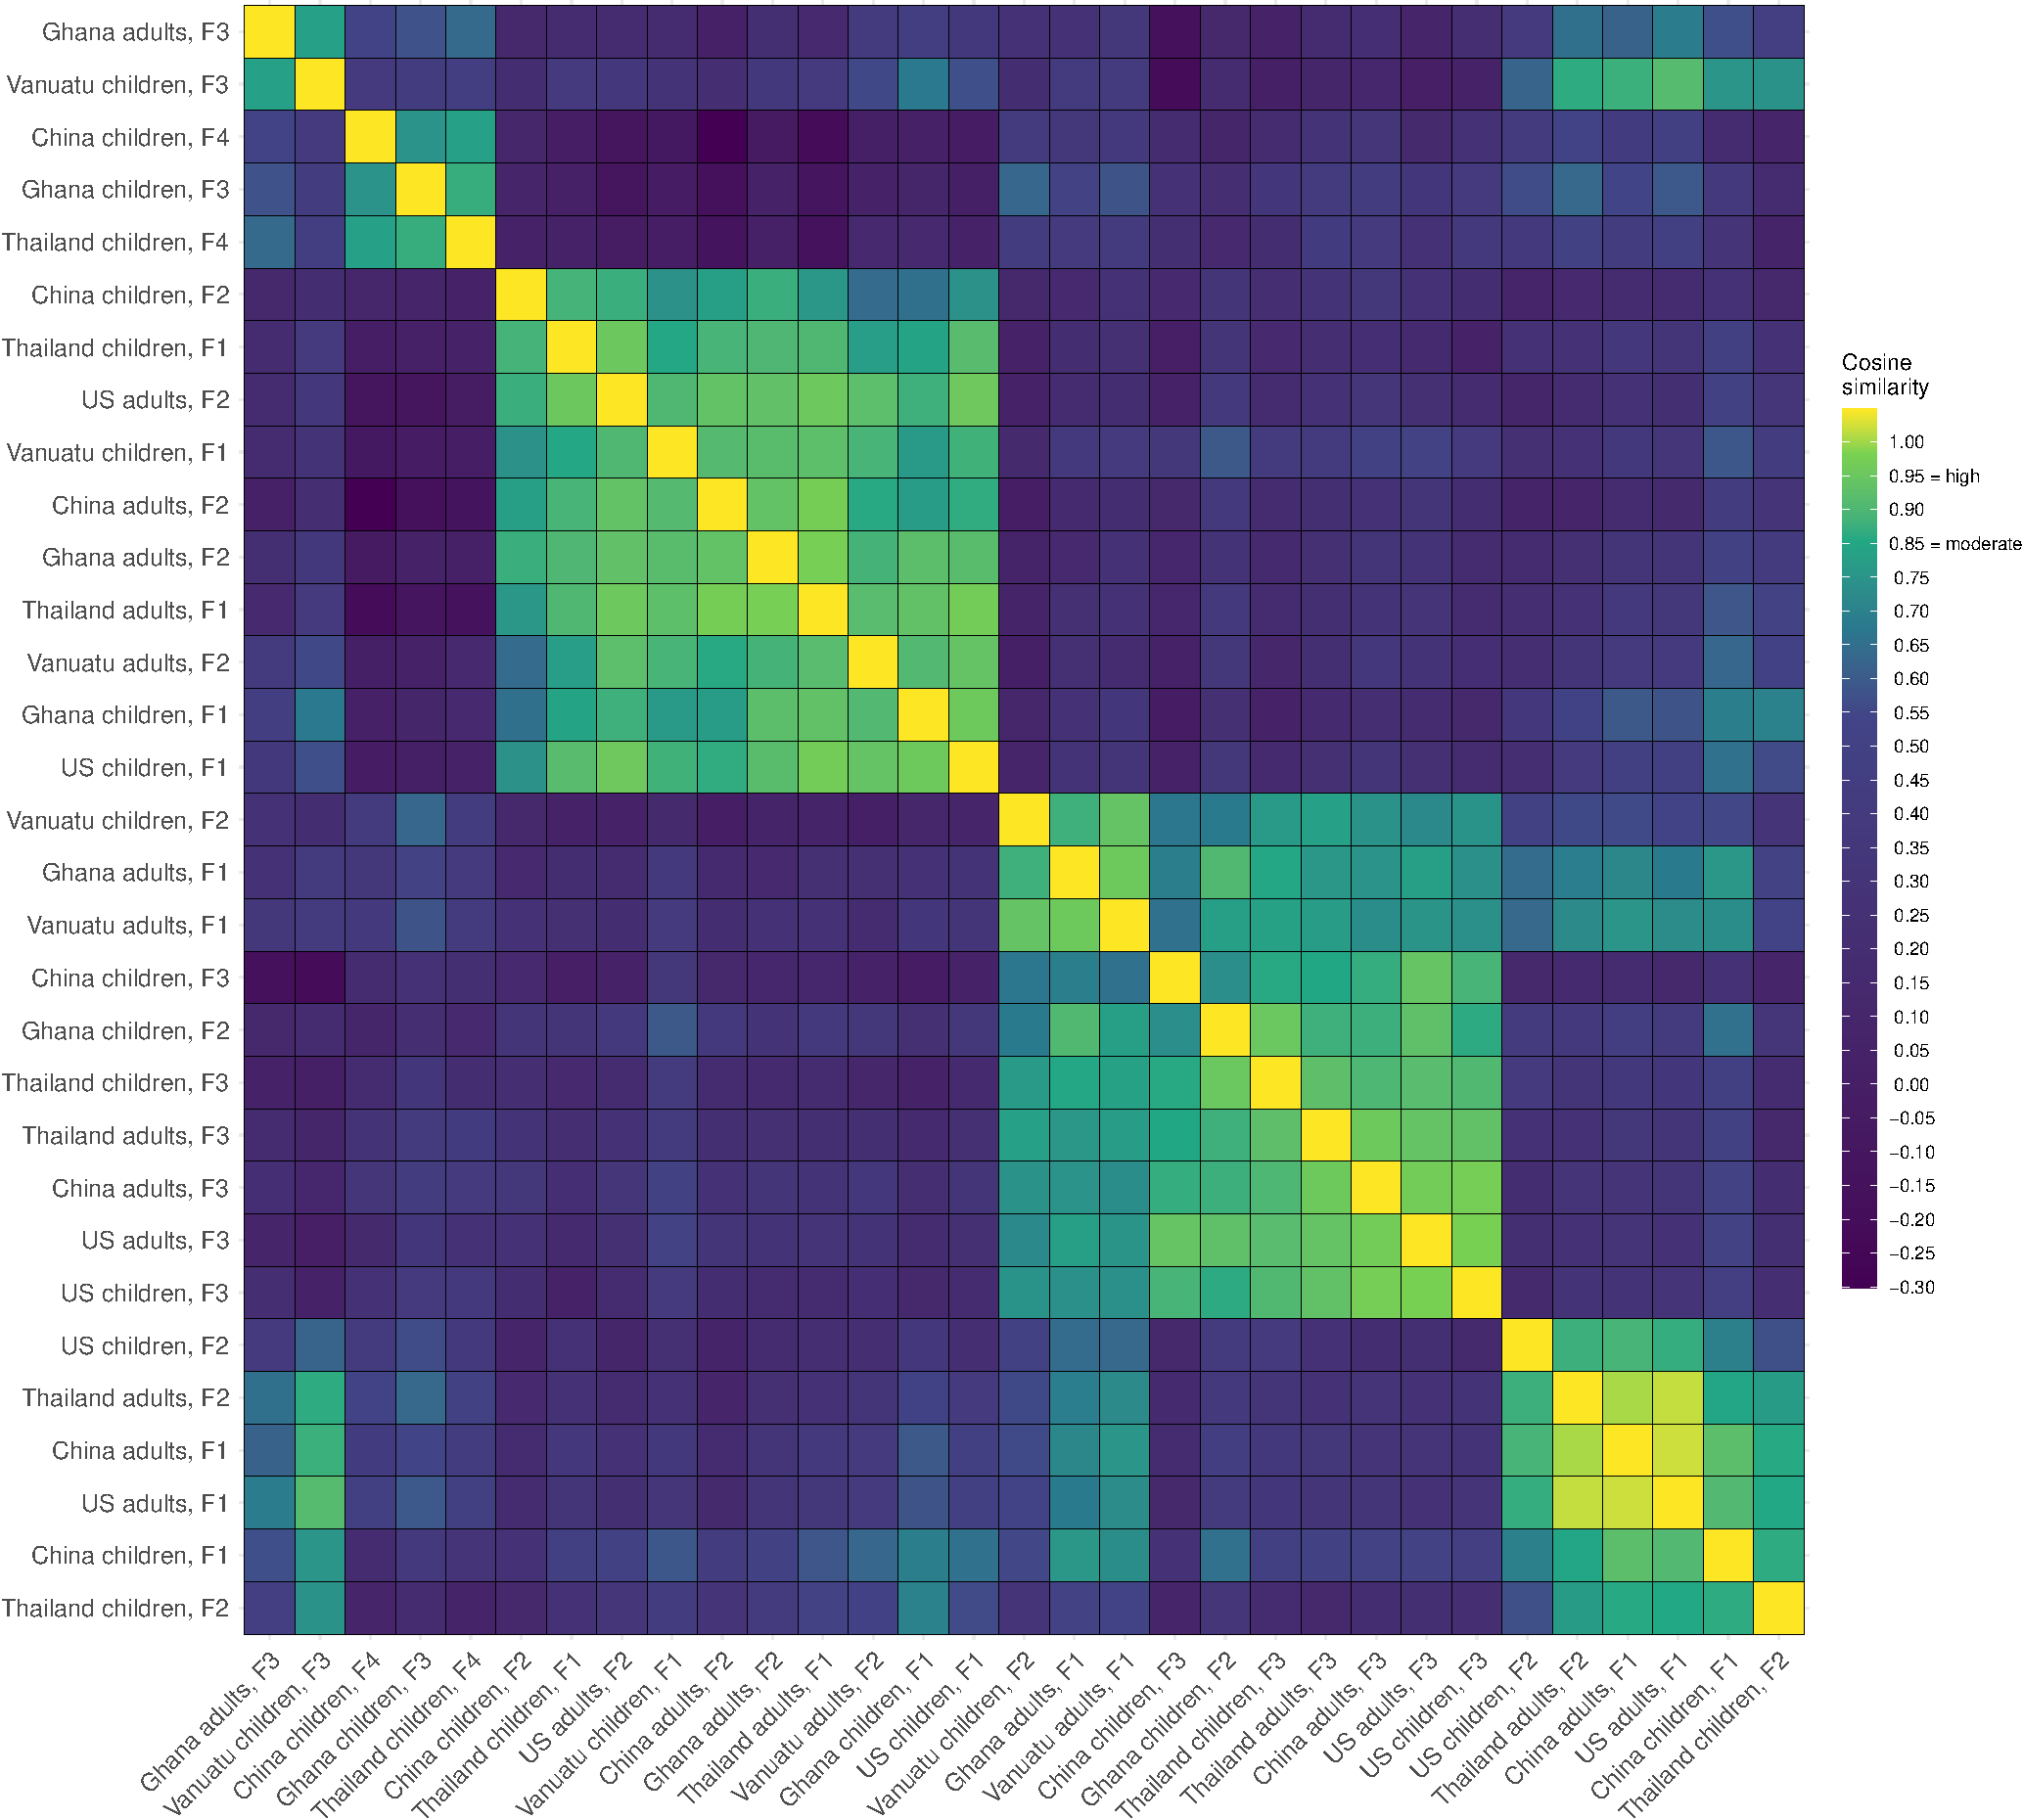
\includegraphics{Script_Re_Weisman_2021_Group1_2024_files/figure-latex/cong all pairs plot b-1.pdf}

\hypertarget{jaccard-similarity-figure-s1}{%
\subsubsection{Jaccard Similarity: Figure S1}\label{jaccard-similarity-figure-s1}}

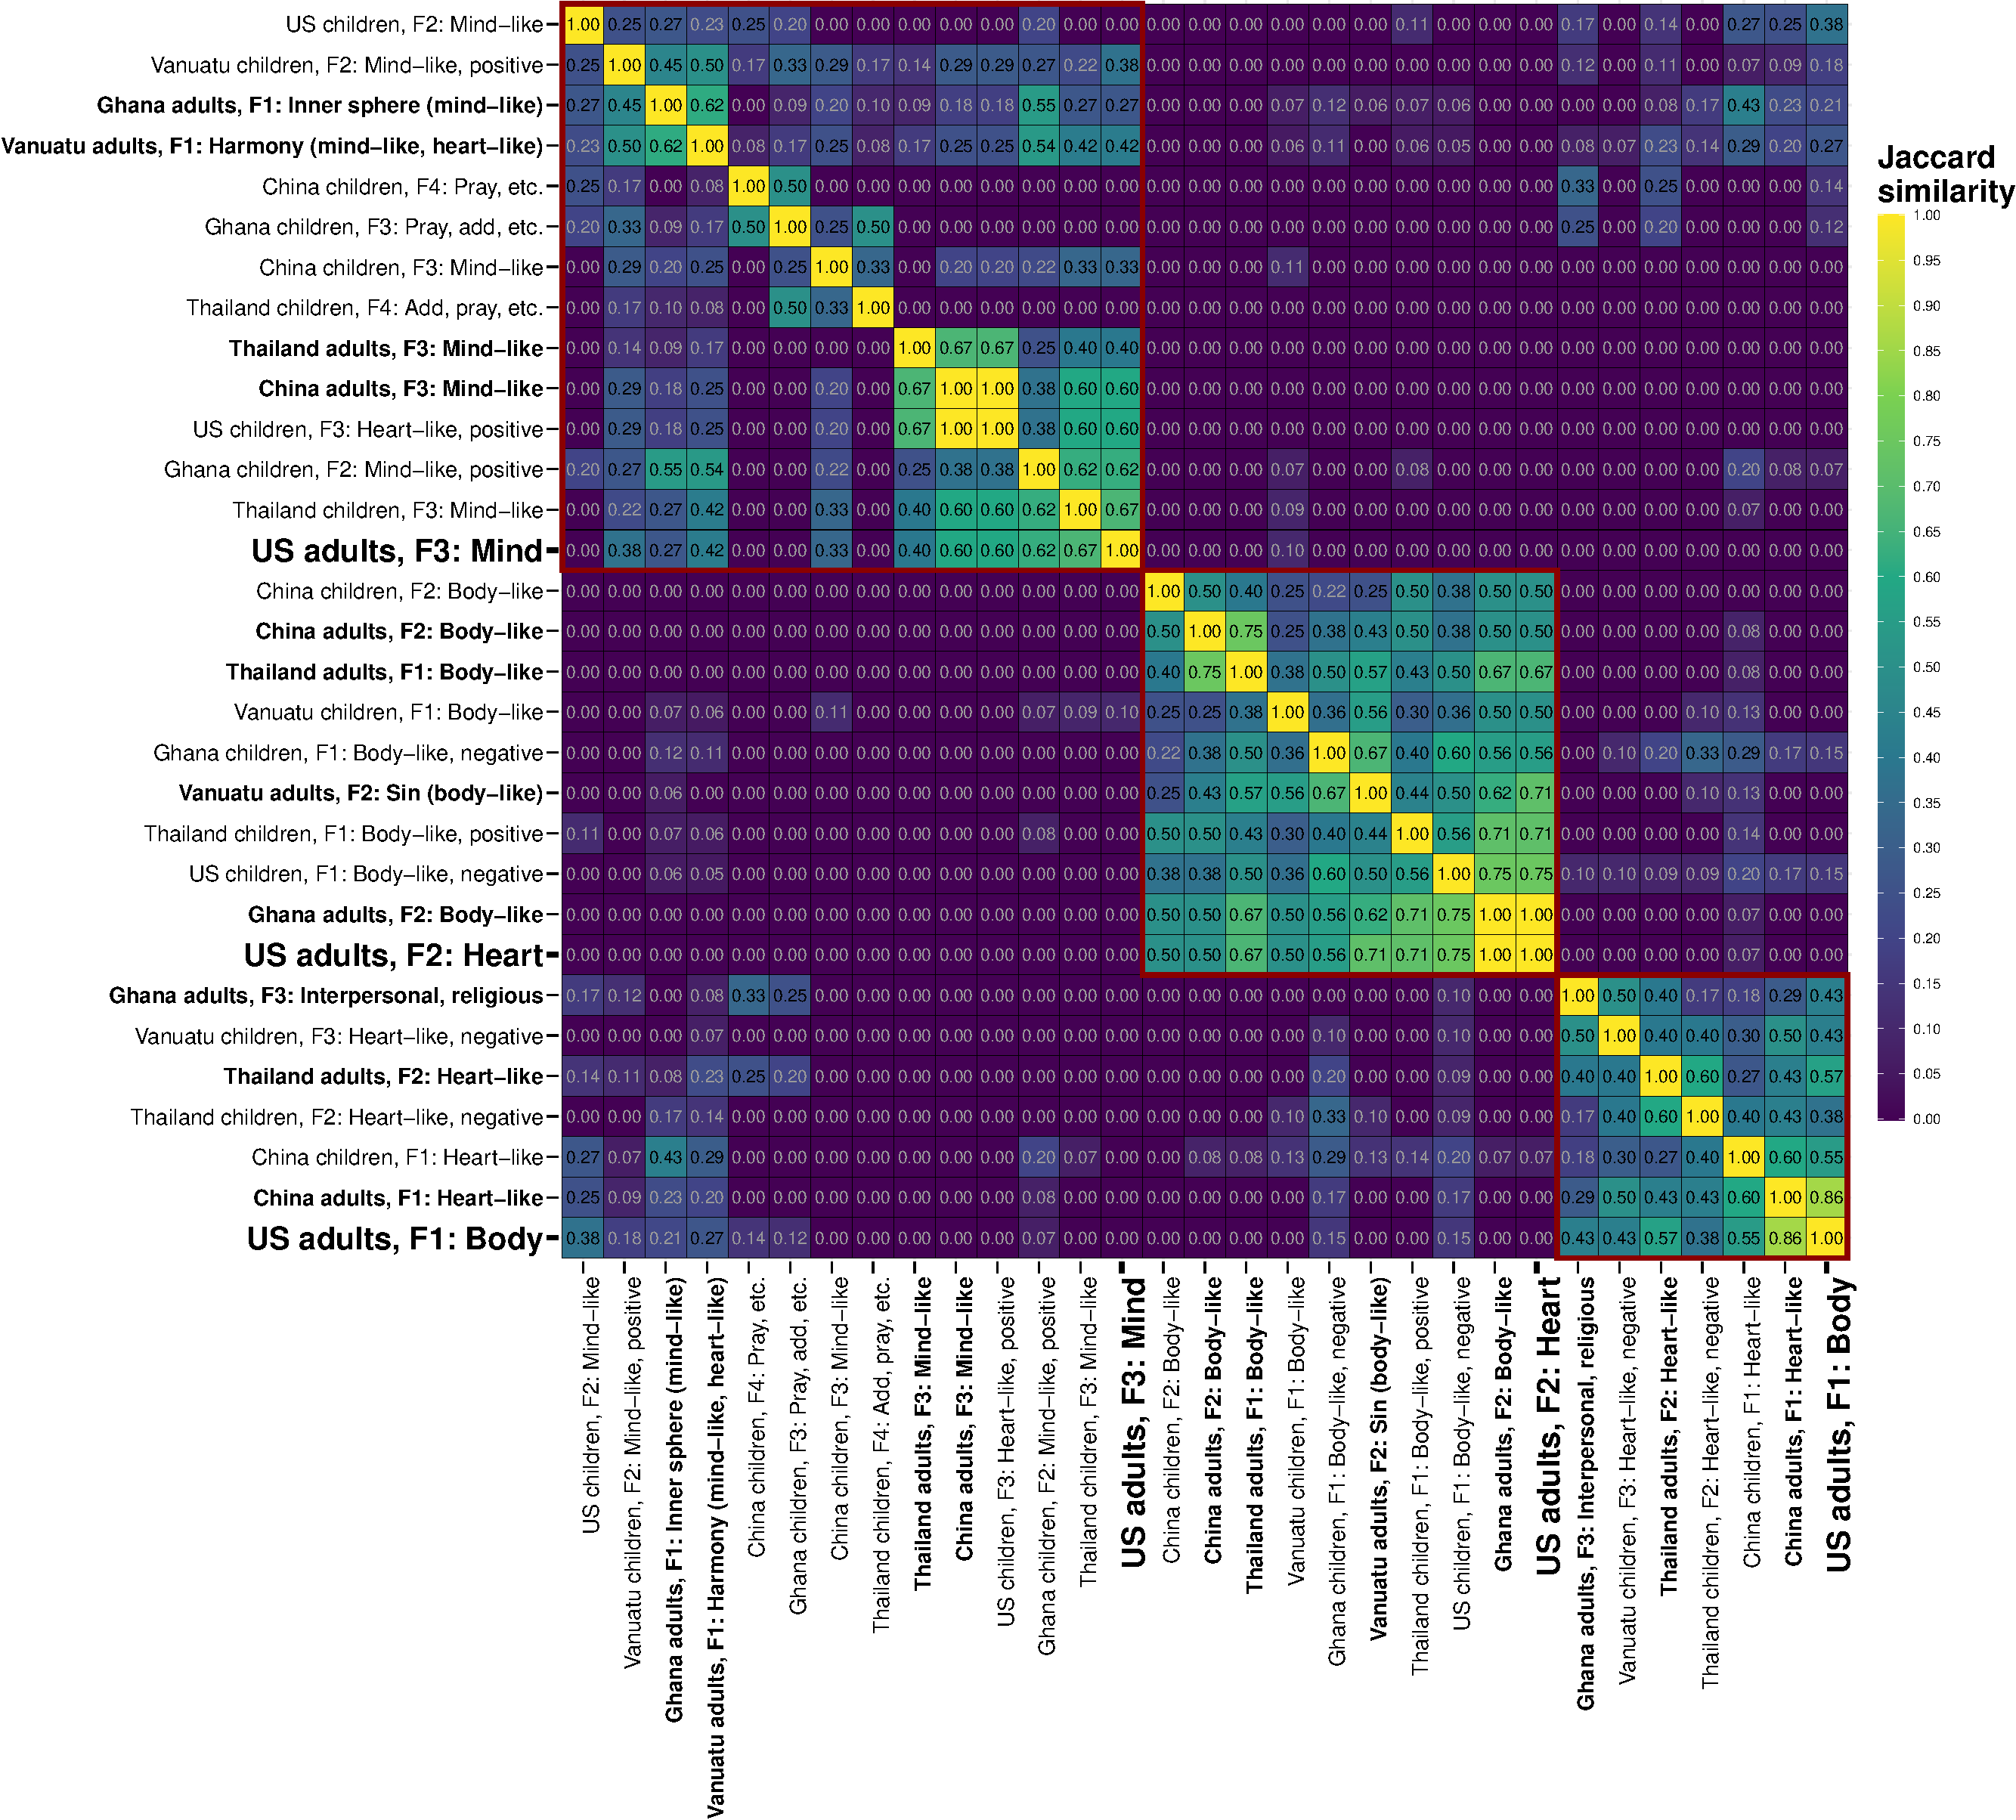
\includegraphics{Script_Re_Weisman_2021_Group1_2024_files/figure-latex/jaccard all pairs plot-1.pdf}

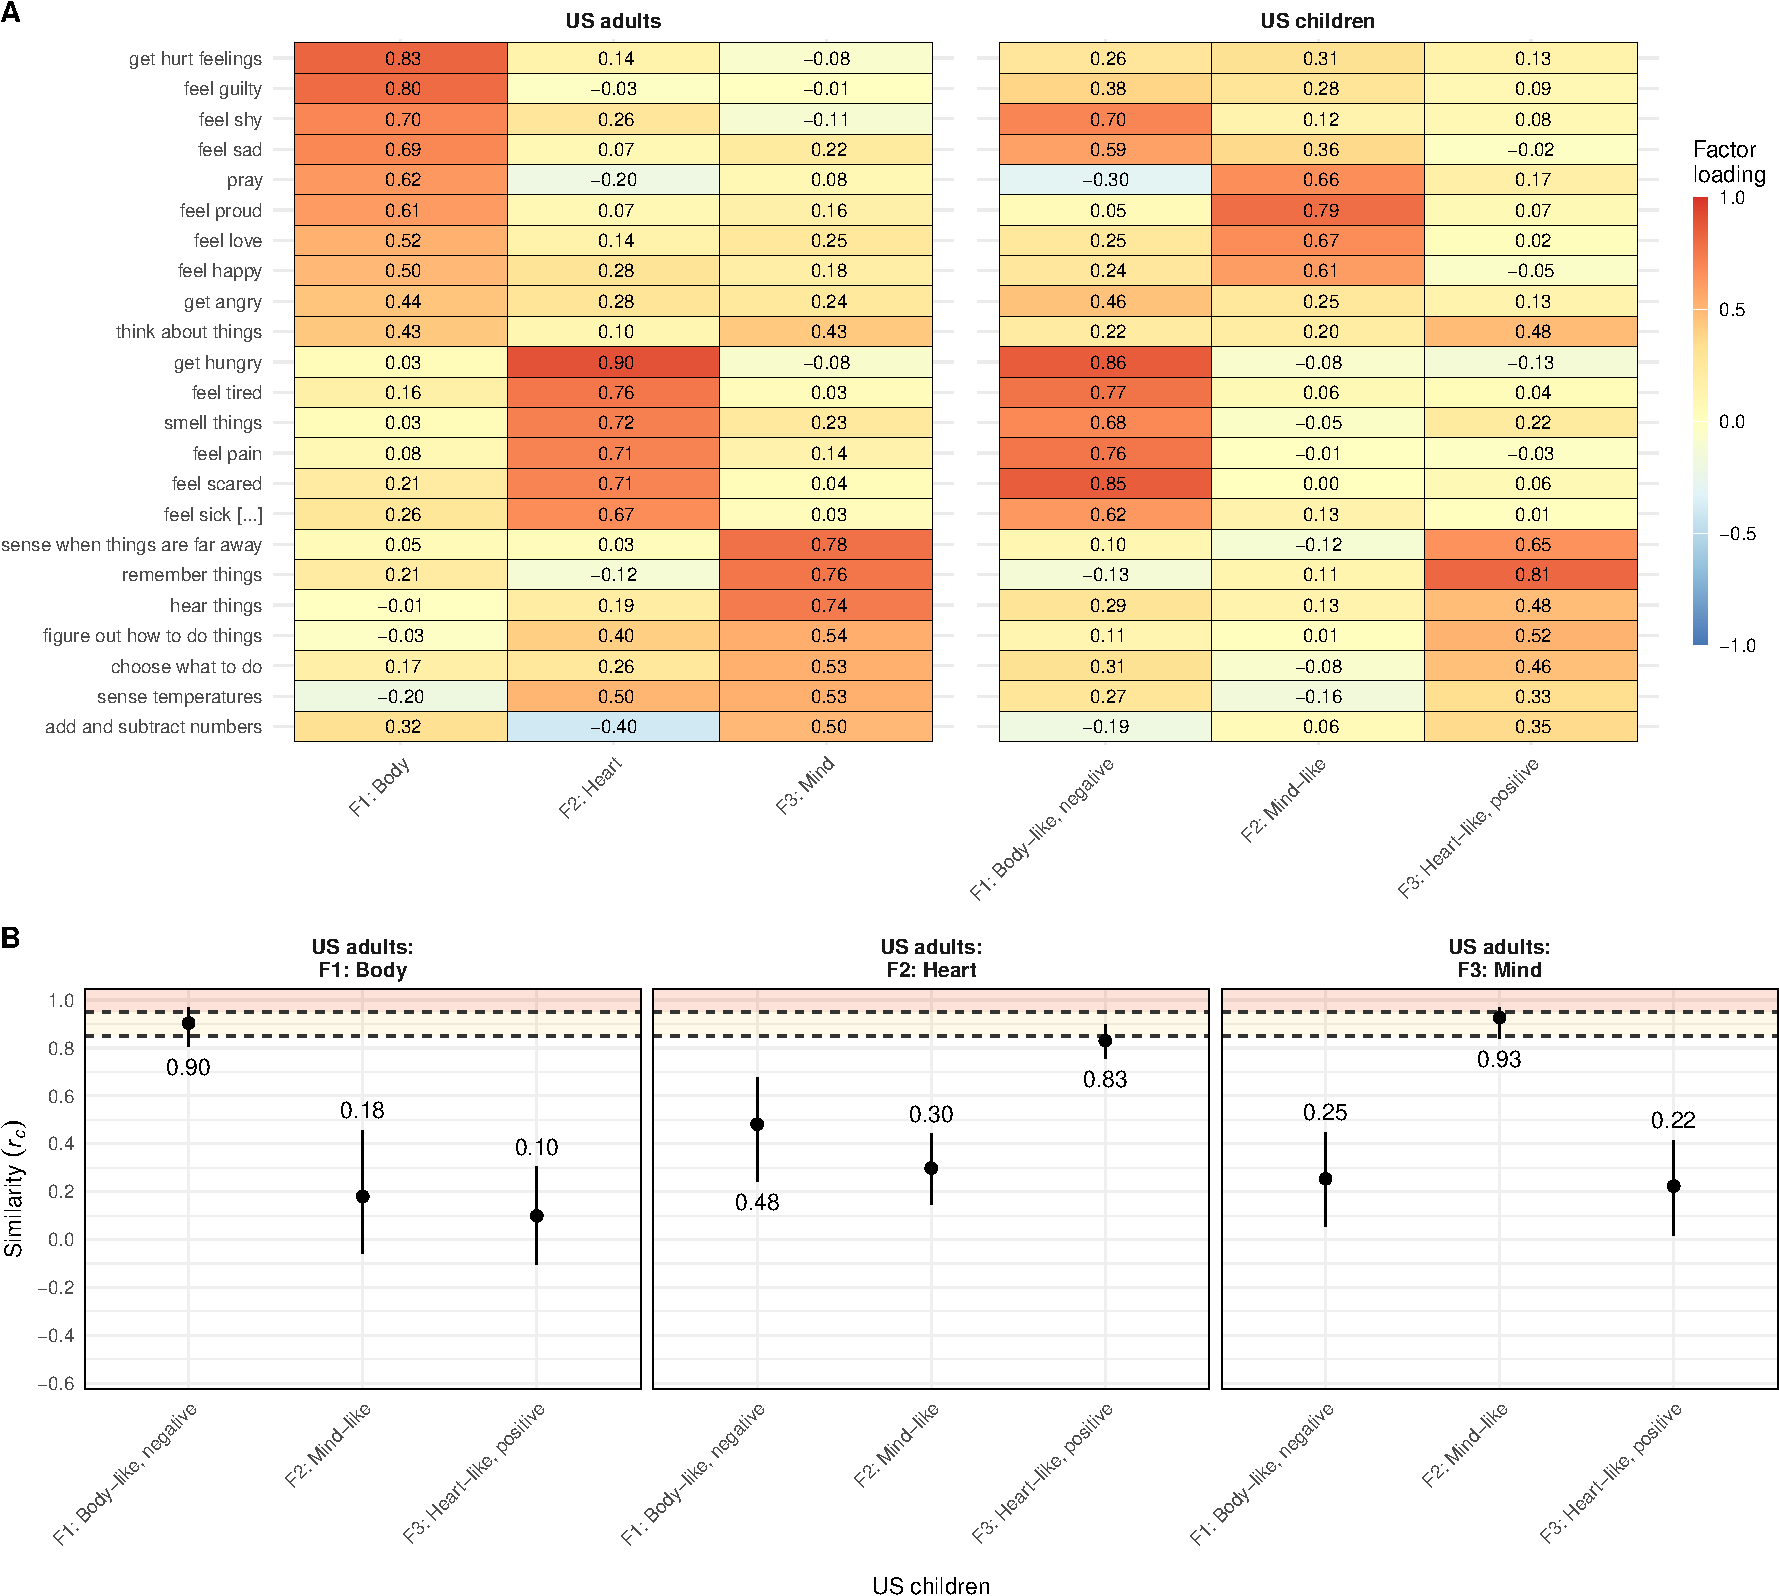
\includegraphics{Script_Re_Weisman_2021_Group1_2024_files/figure-latex/dev comp all sites-1.pdf} 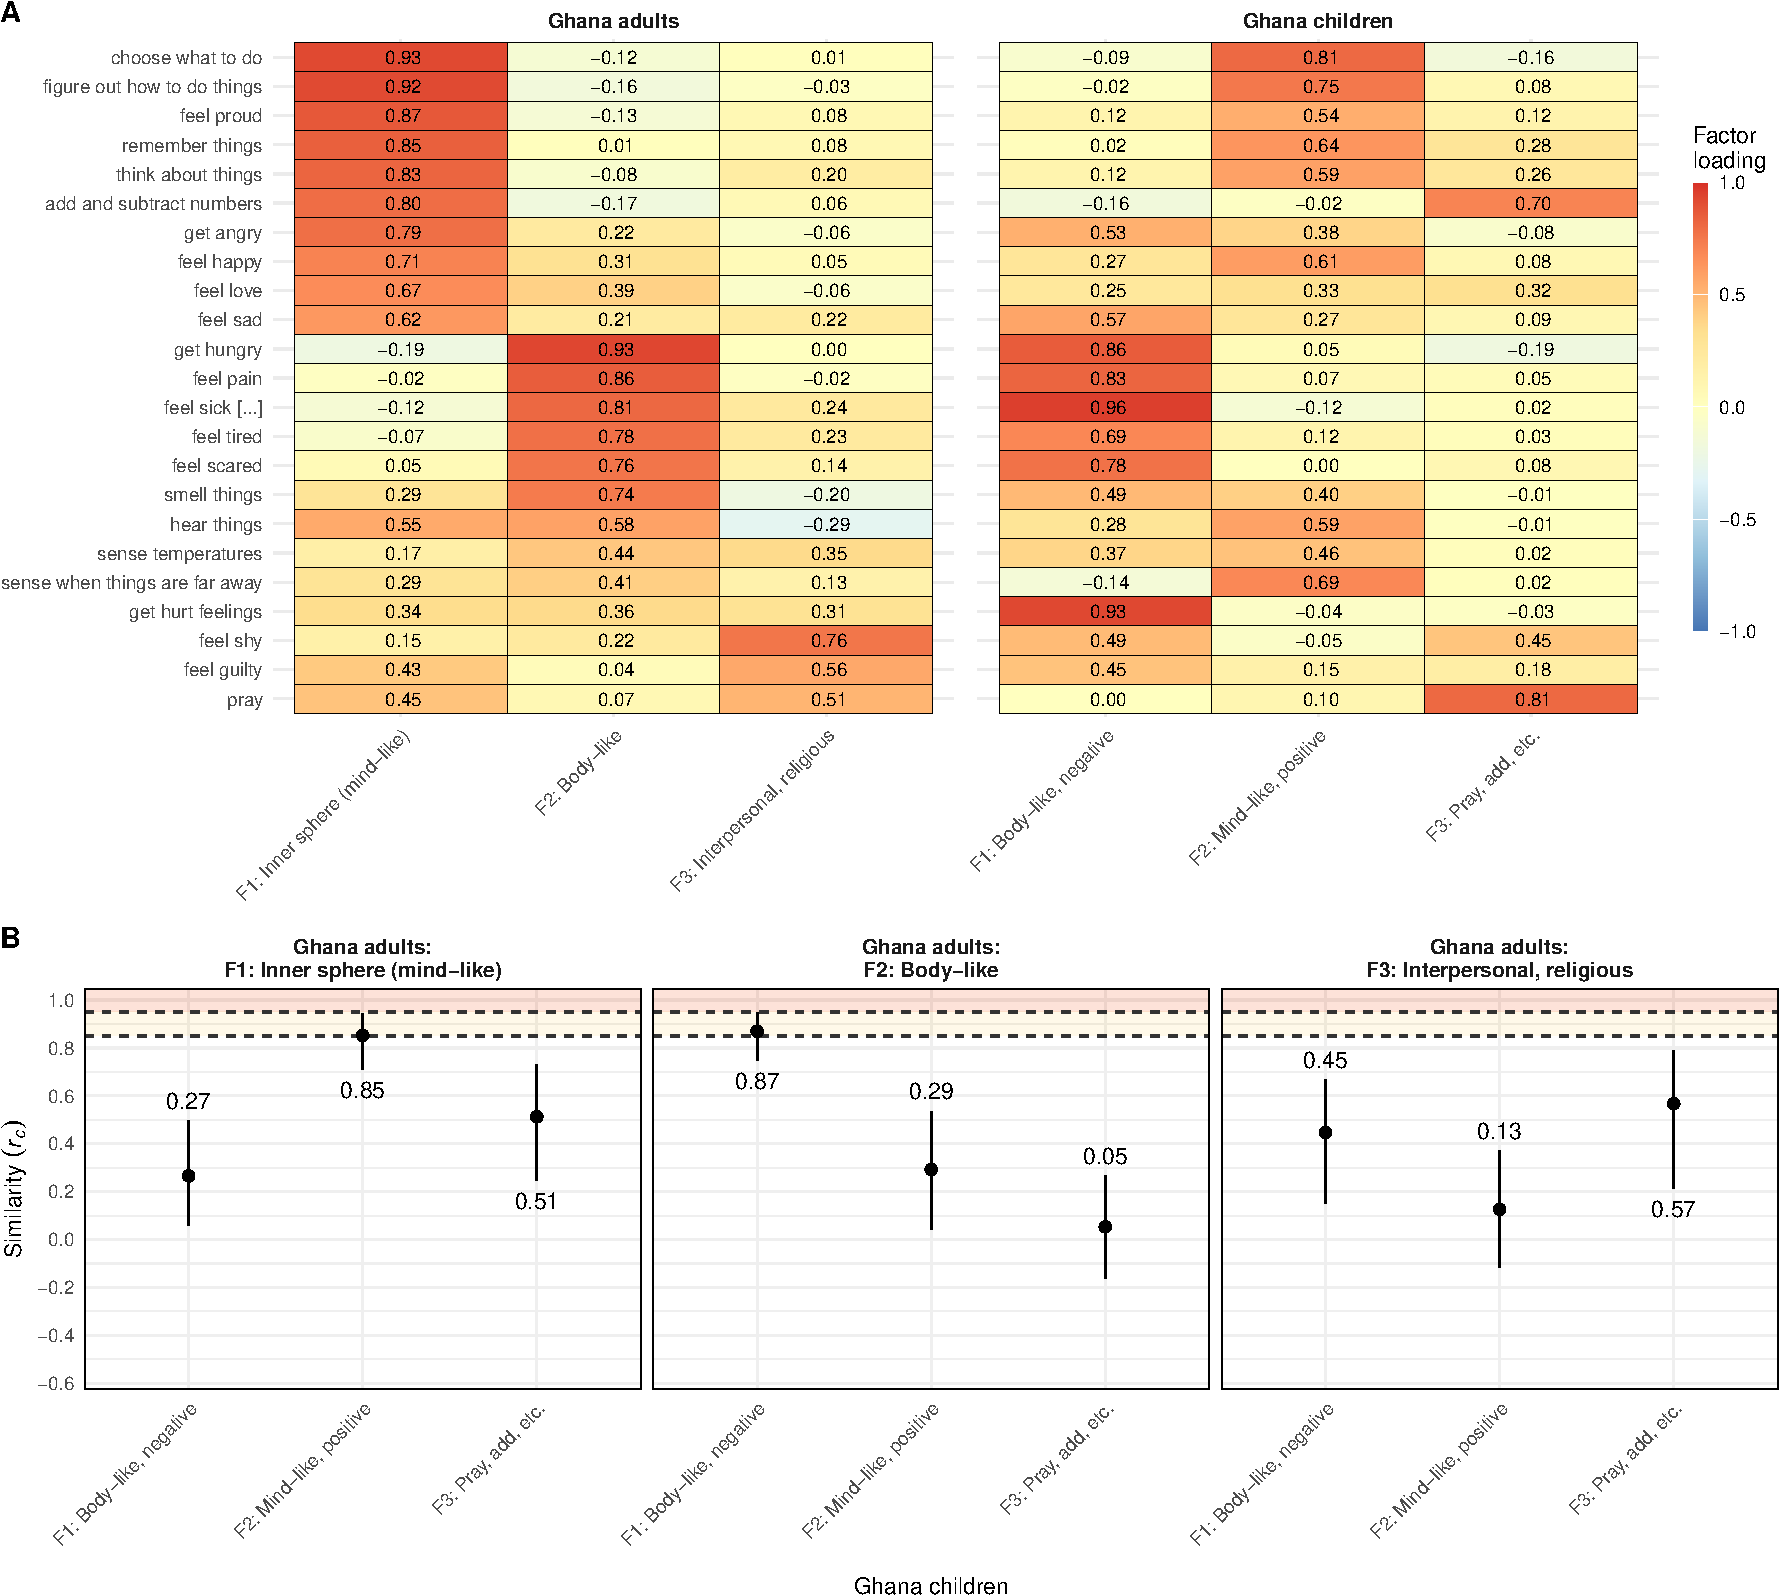
\includegraphics{Script_Re_Weisman_2021_Group1_2024_files/figure-latex/dev comp all sites-2.pdf} 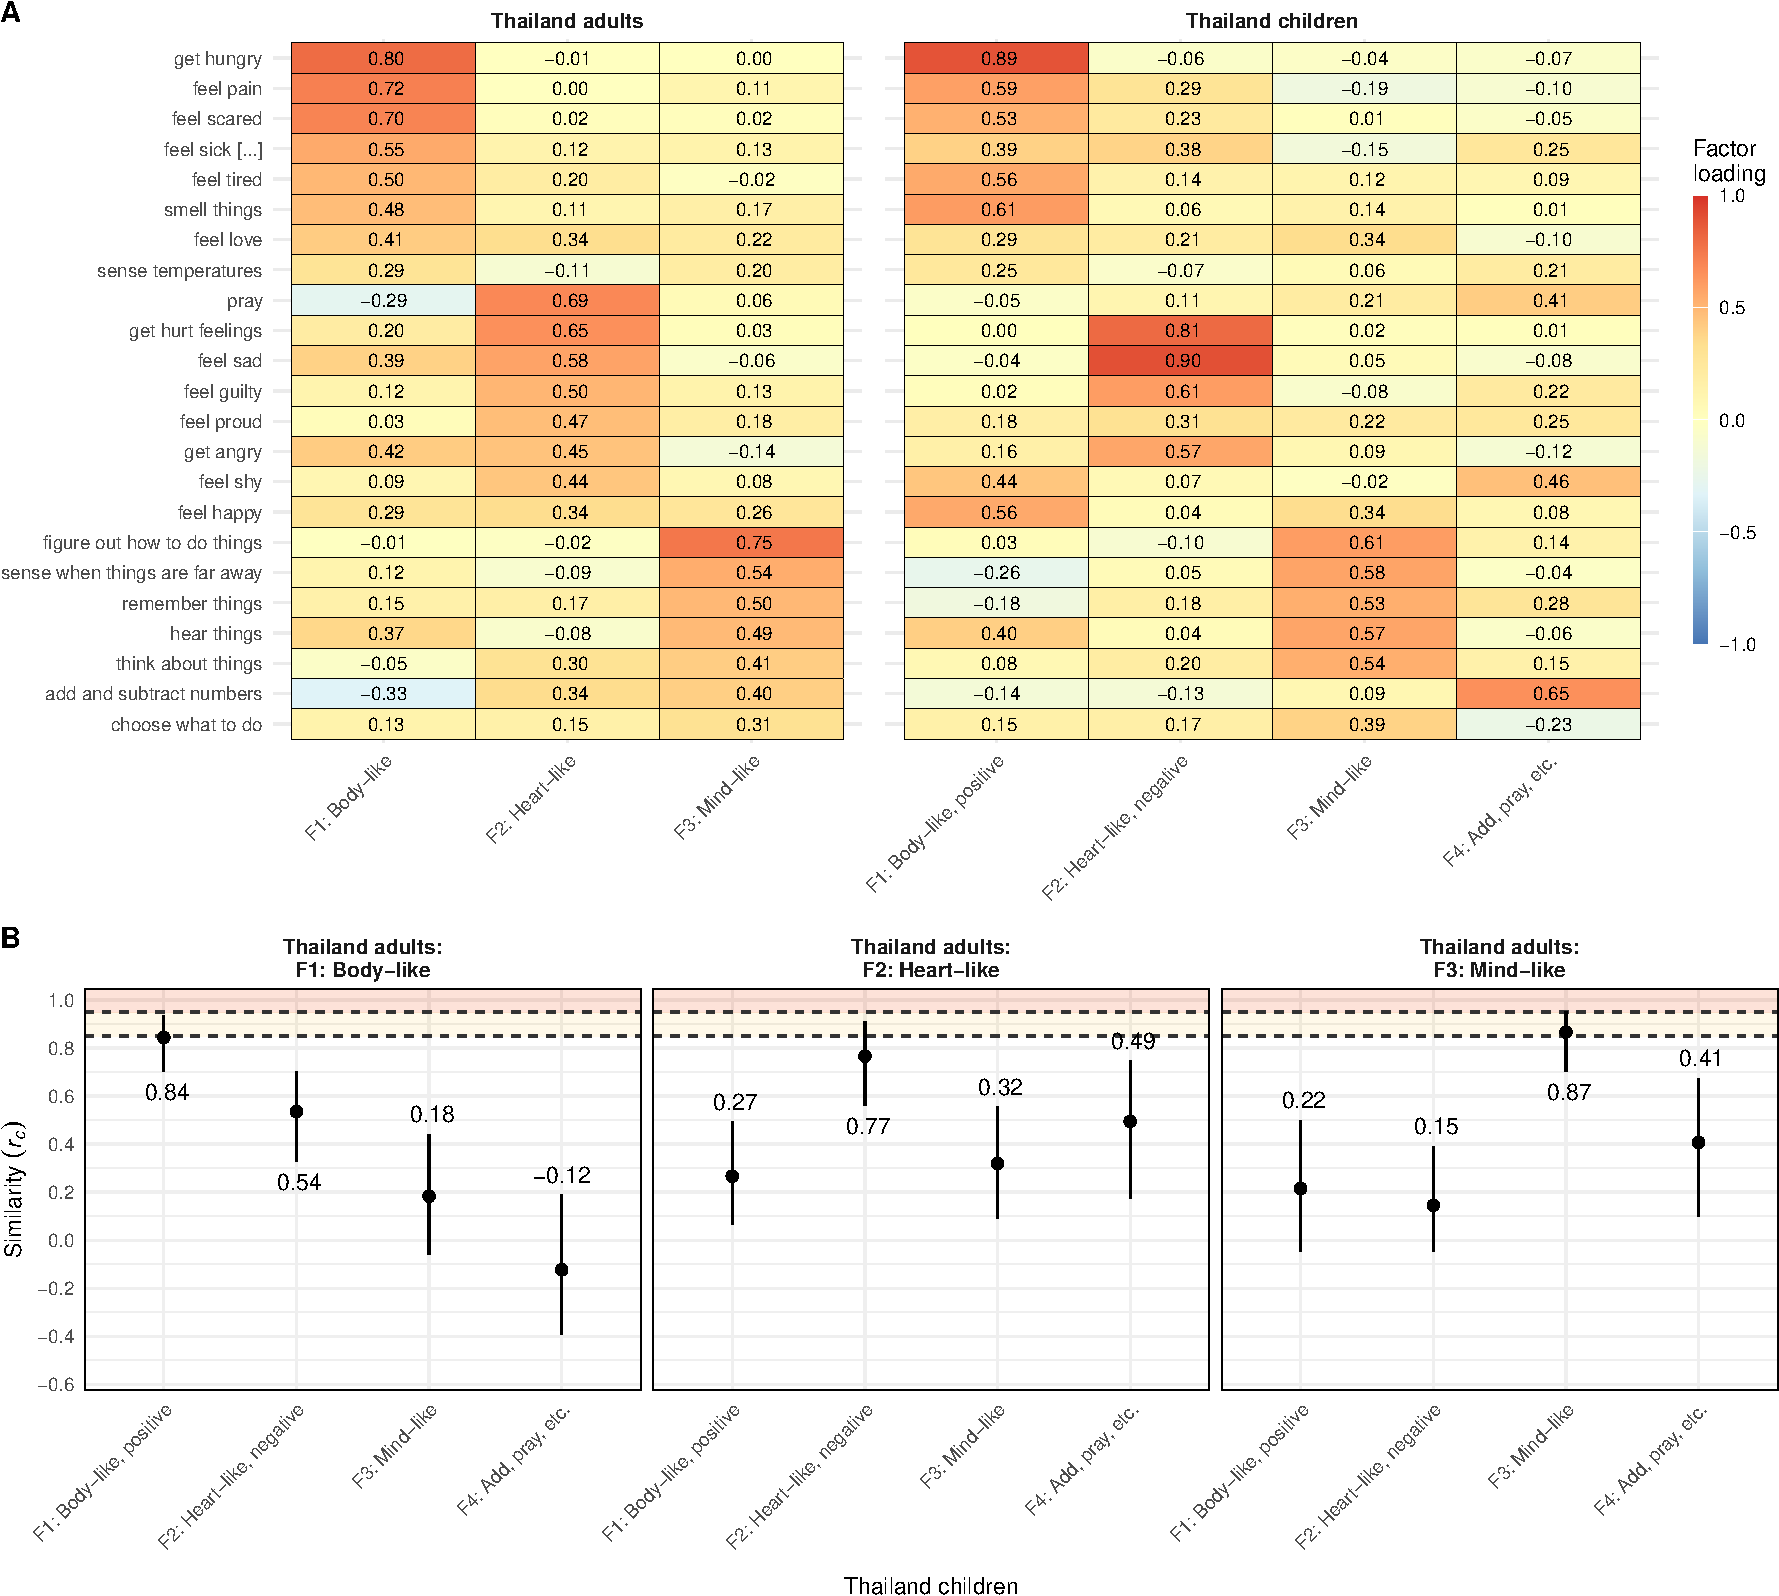
\includegraphics{Script_Re_Weisman_2021_Group1_2024_files/figure-latex/dev comp all sites-3.pdf} 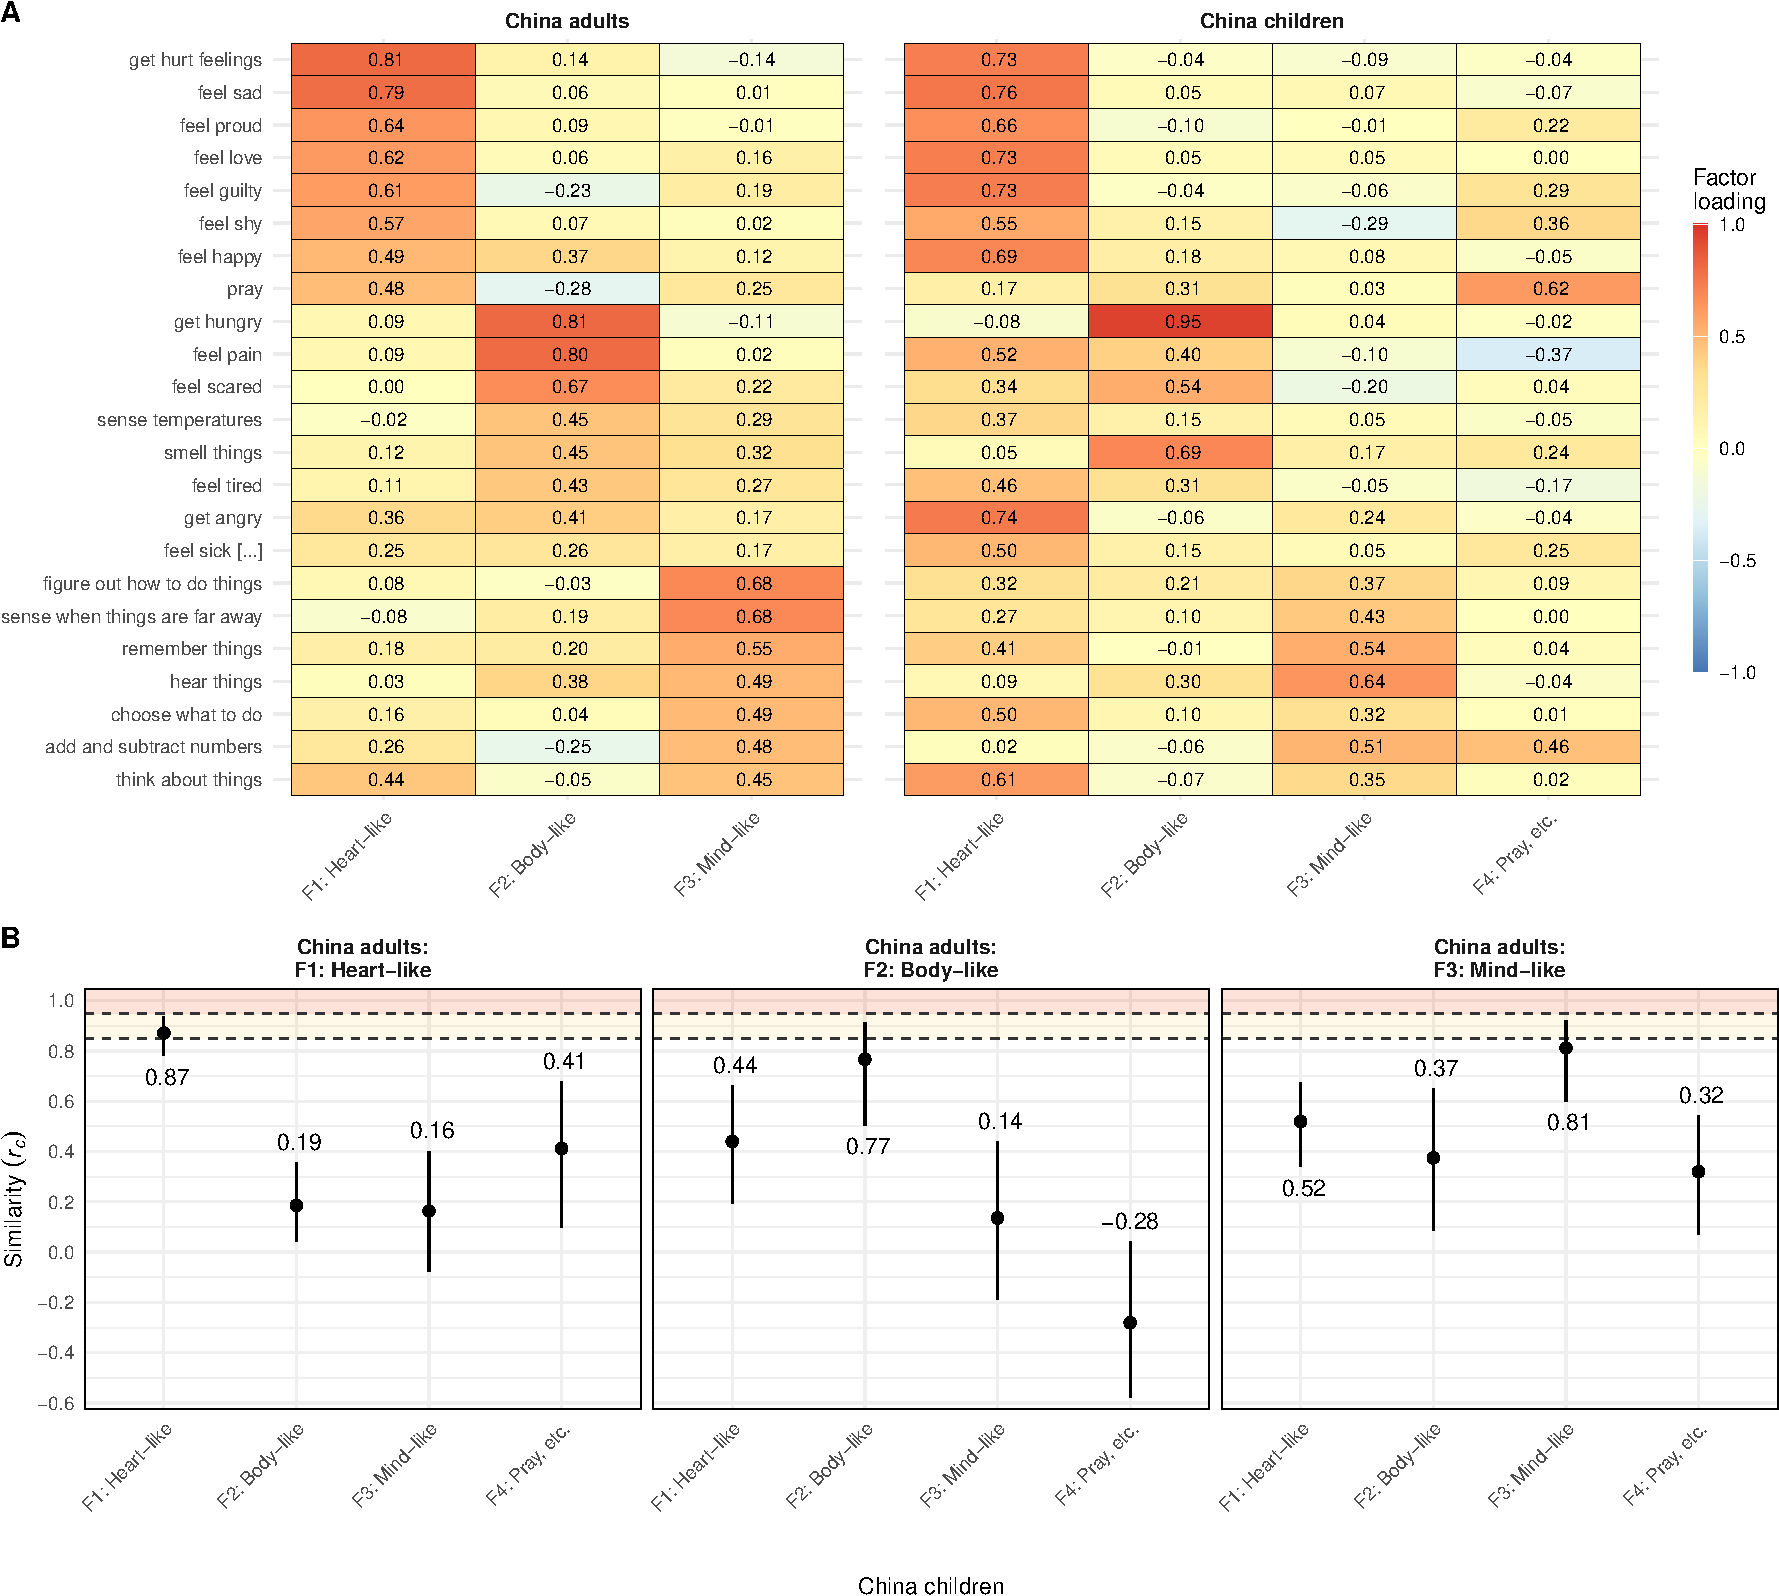
\includegraphics{Script_Re_Weisman_2021_Group1_2024_files/figure-latex/dev comp all sites-4.pdf} 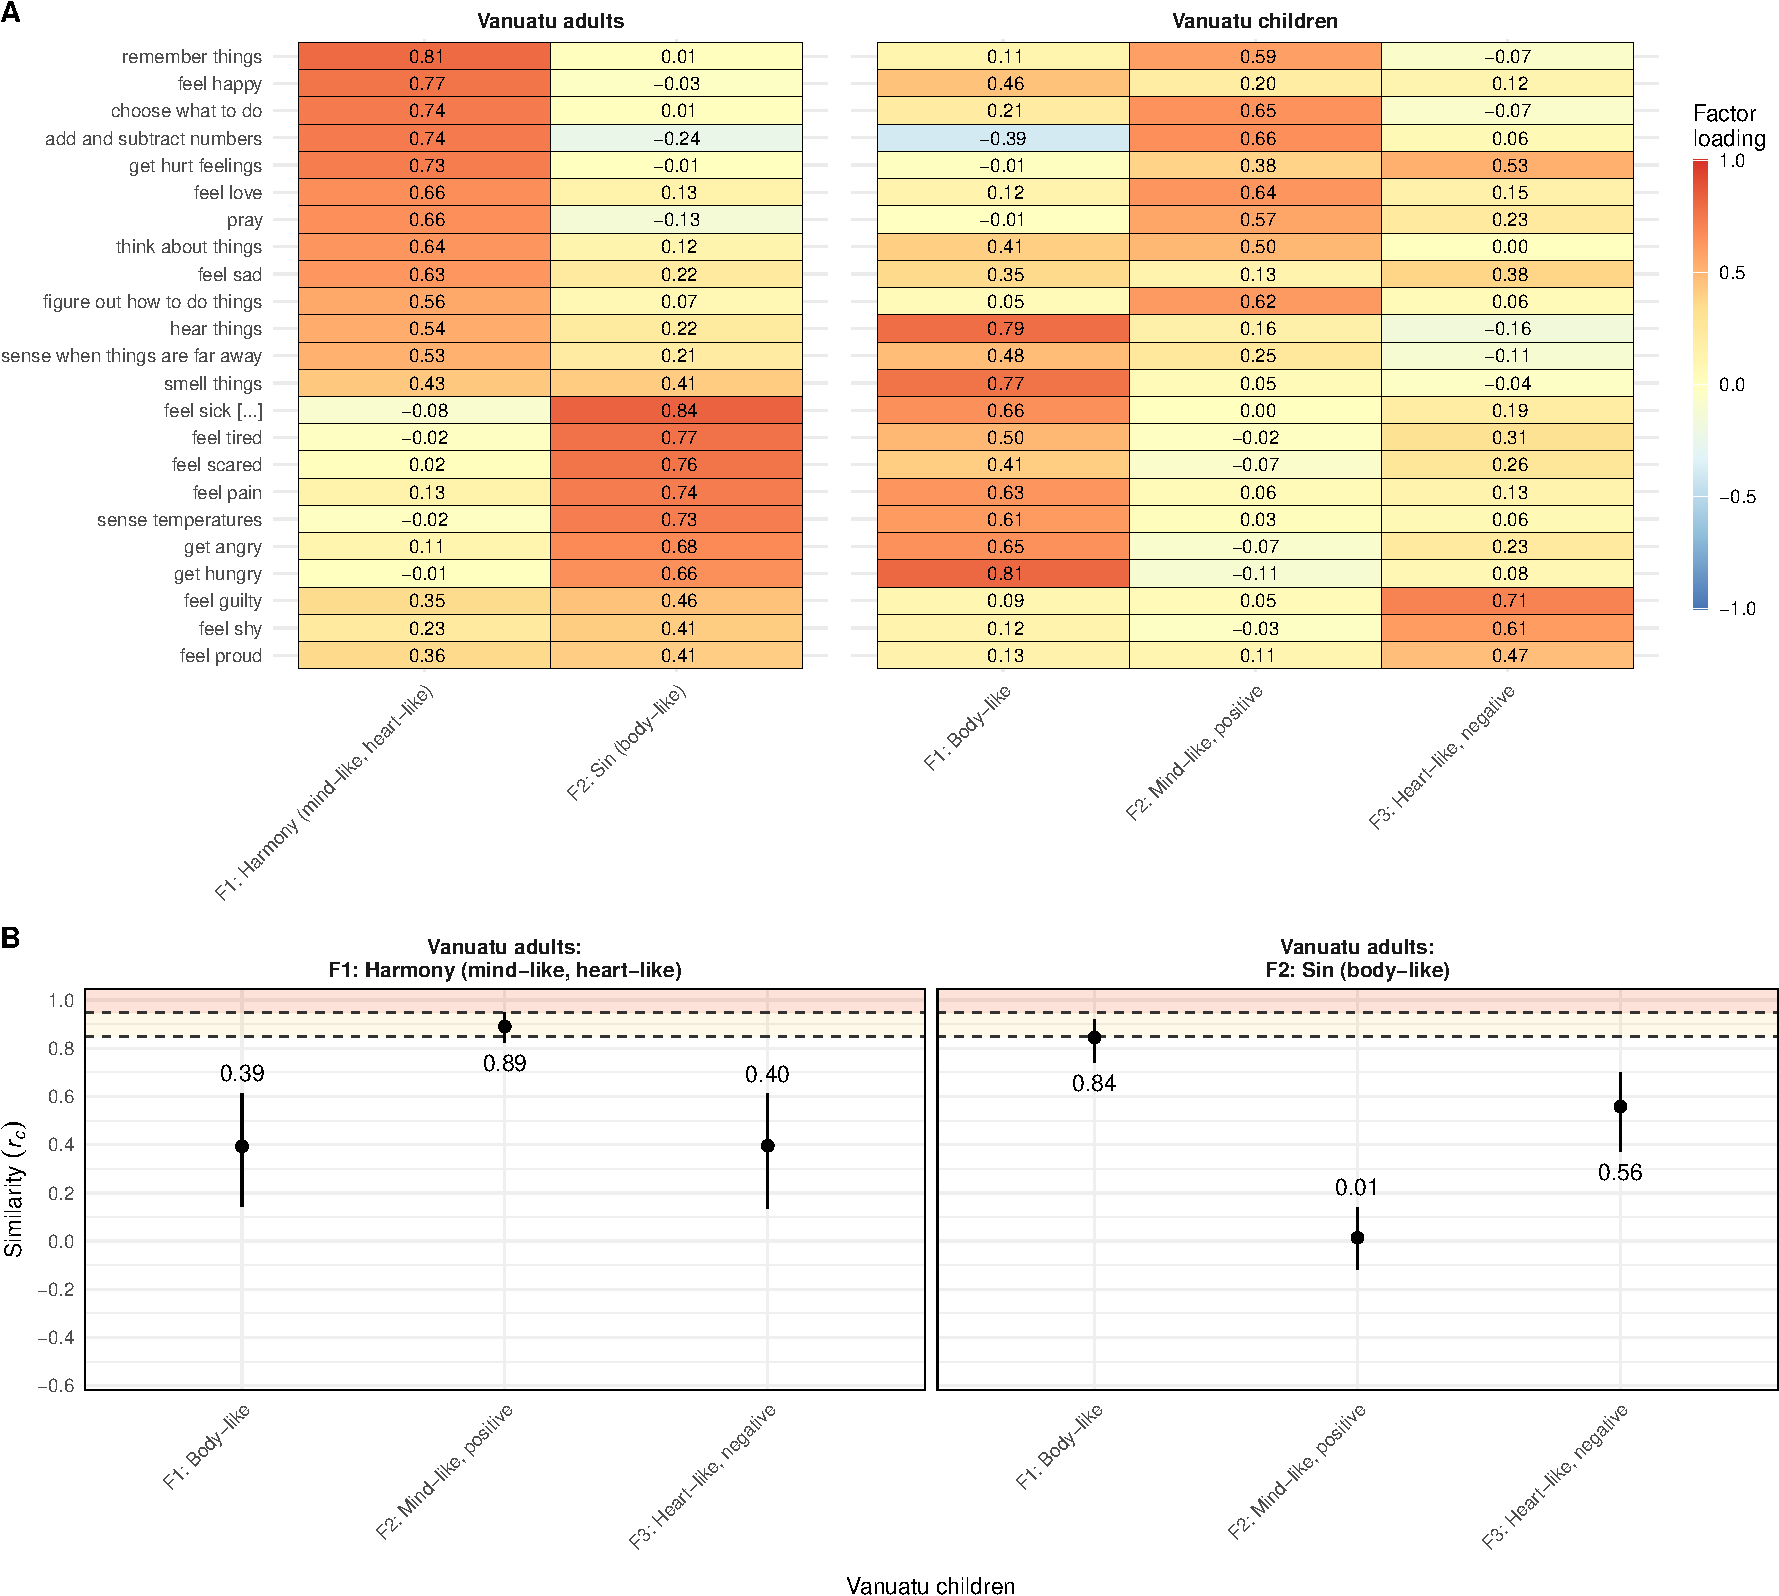
\includegraphics{Script_Re_Weisman_2021_Group1_2024_files/figure-latex/dev comp all sites-5.pdf}

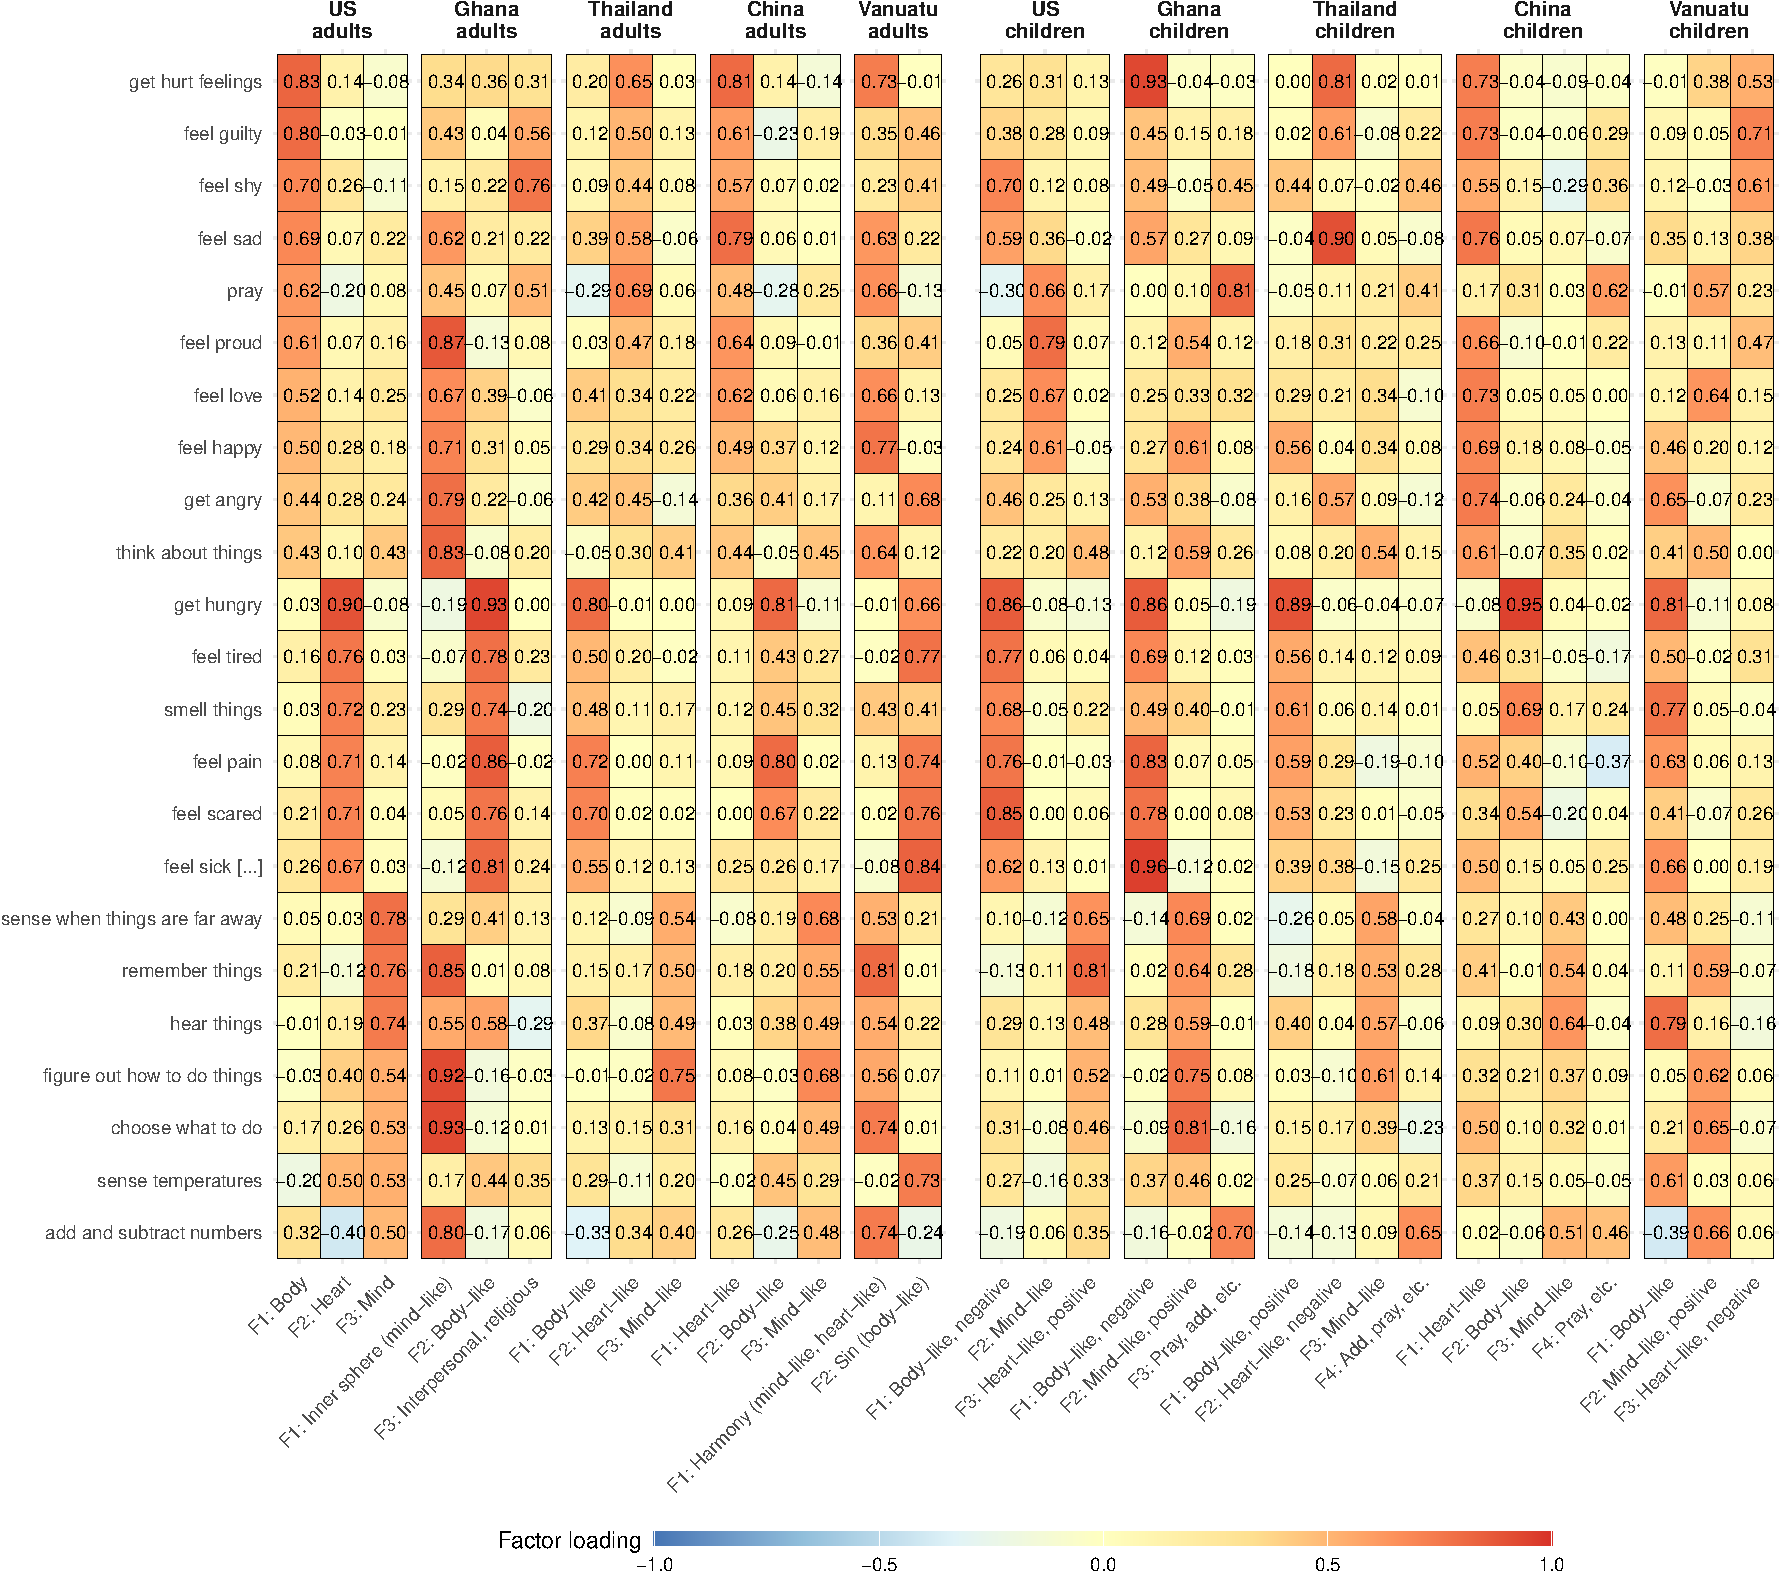
\includegraphics{Script_Re_Weisman_2021_Group1_2024_files/figure-latex/loadings all samples-1.pdf}

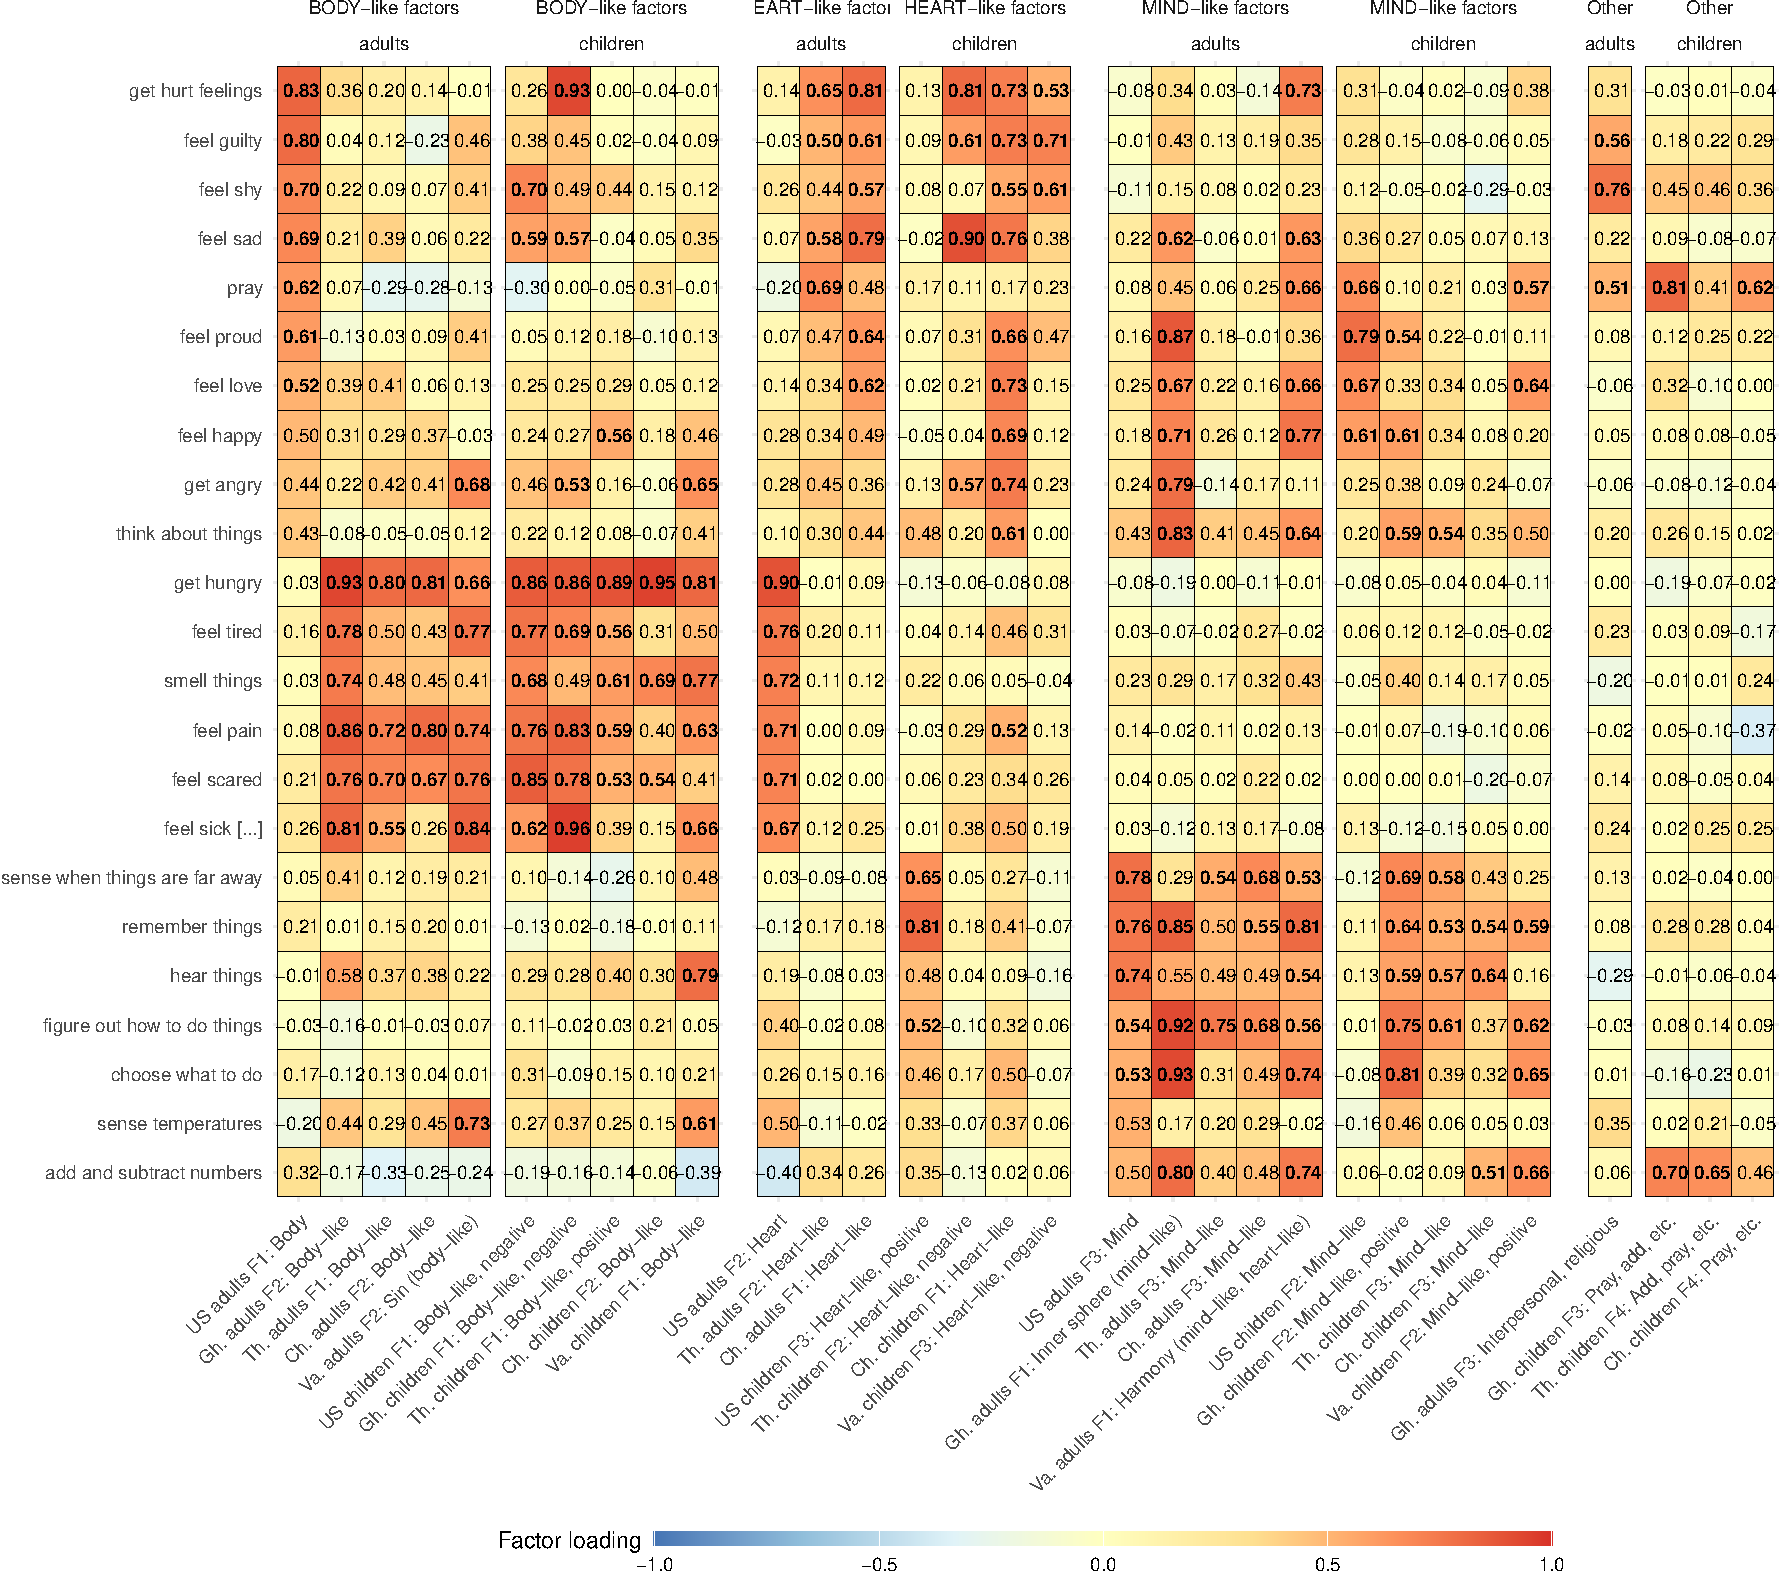
\includegraphics{Script_Re_Weisman_2021_Group1_2024_files/figure-latex/loadings all samples v2a-1.pdf}

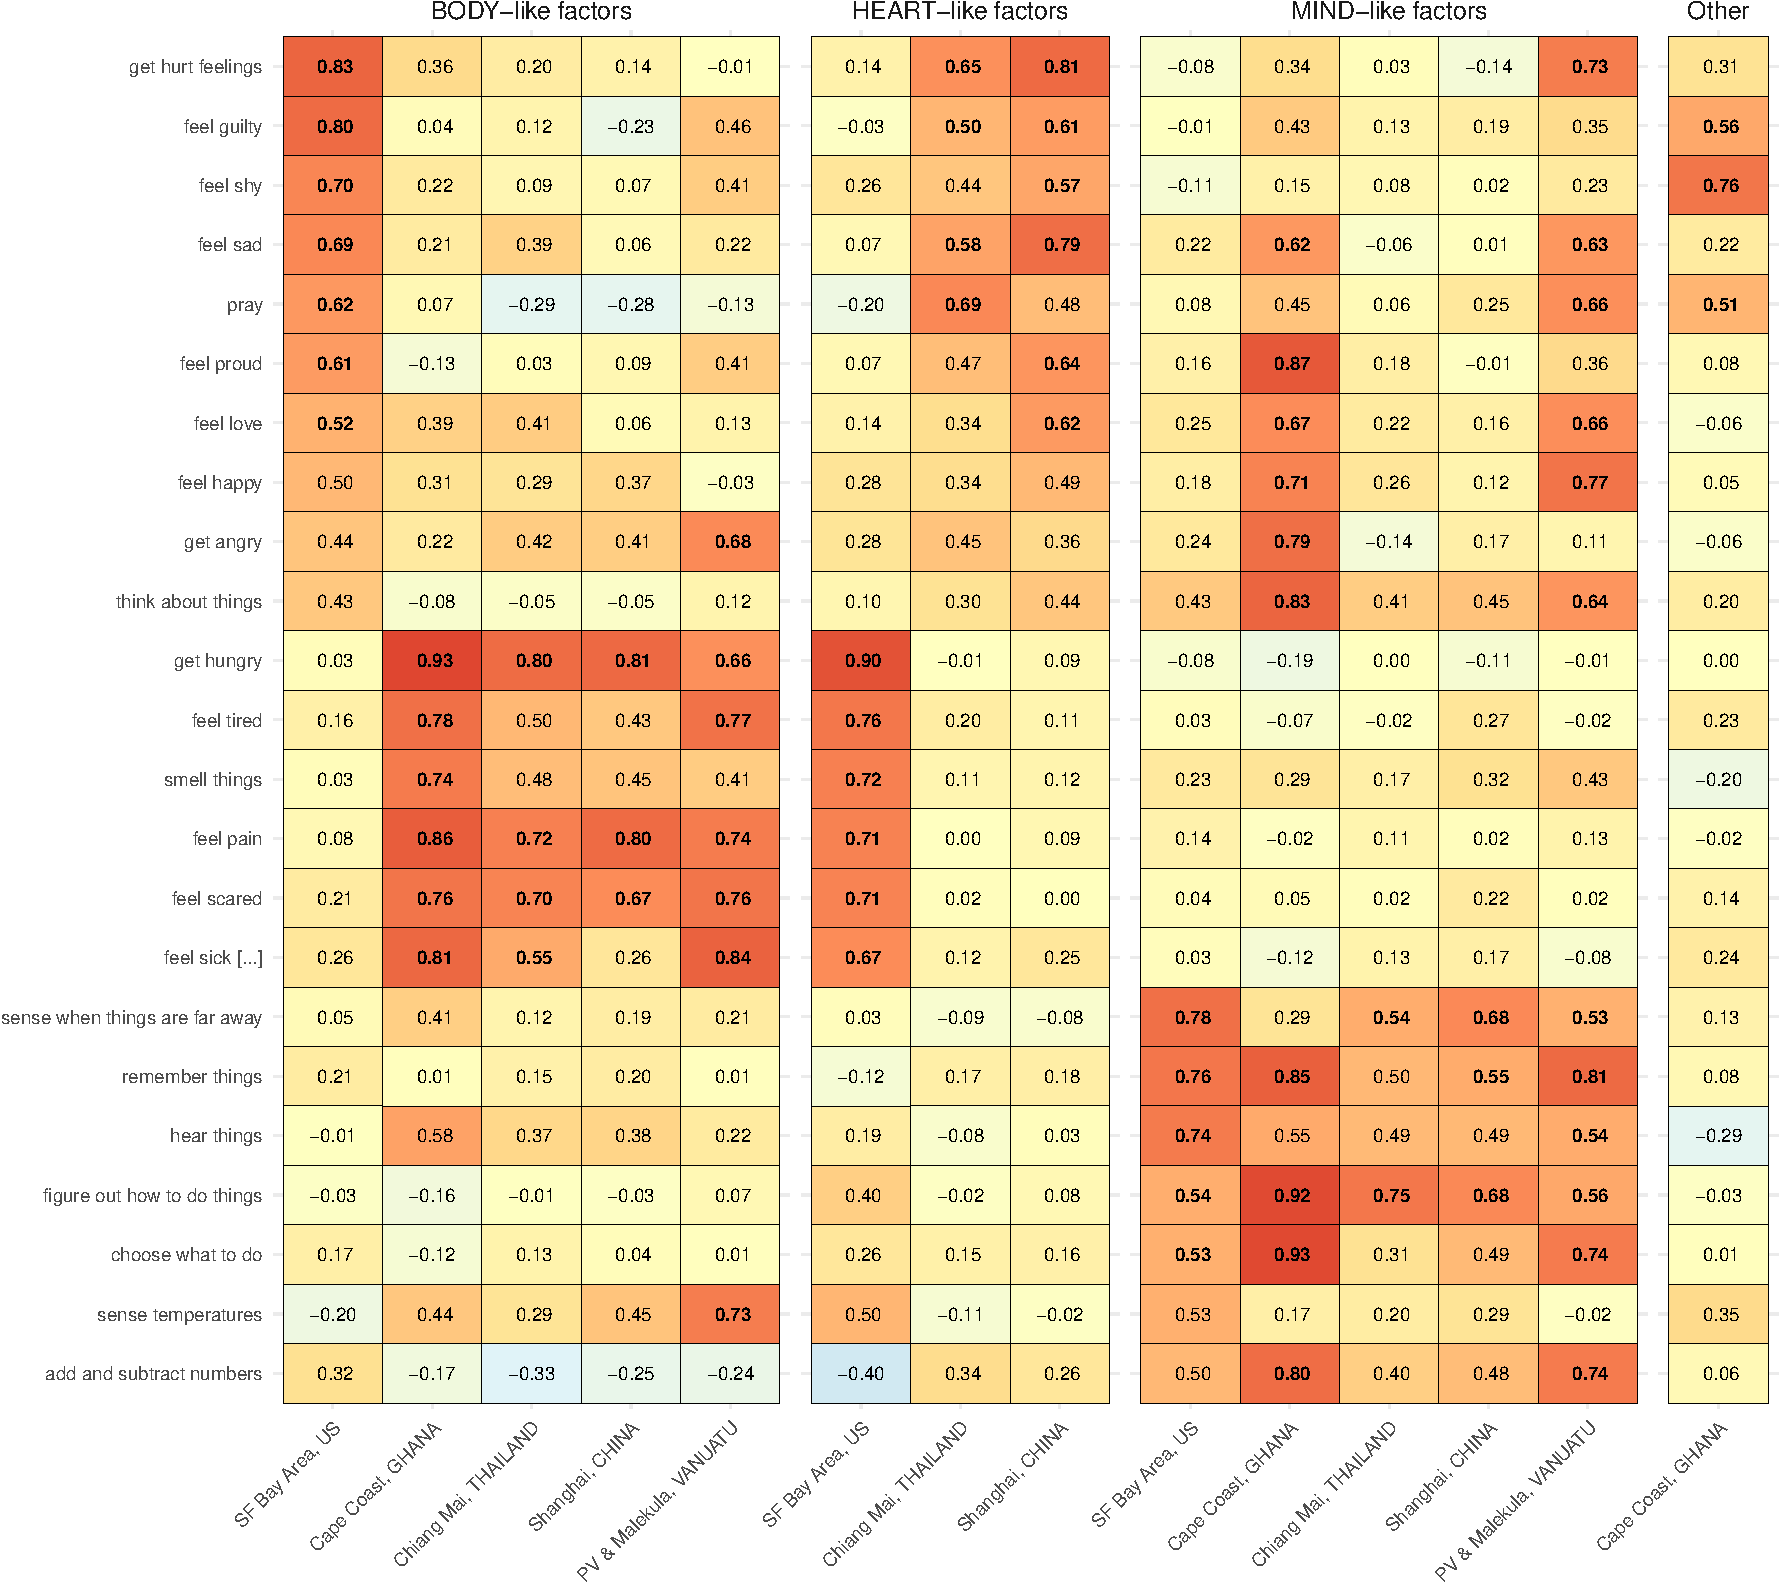
\includegraphics{Script_Re_Weisman_2021_Group1_2024_files/figure-latex/loadings all samples v2b-1.pdf}

\begin{verbatim}
##                  metric age_group factor   US Ghana Thailand China Vanuatu
## 1  Proportion Explained    adults     F1 0.36  0.50     0.41  0.39    0.55
## 2        Proportion Var    adults     F1 0.23  0.35     0.18  0.20    0.29
## 3  Proportion Explained    adults     F2 0.35  0.36     0.33  0.31    0.45
## 4        Proportion Var    adults     F2 0.23  0.25     0.14  0.16    0.24
## 5  Proportion Explained    adults     F3 0.29  0.14     0.26  0.30      NA
## 6        Proportion Var    adults     F3 0.19  0.10     0.11  0.15      NA
## 7  Proportion Explained    adults     F4   NA    NA       NA    NA      NA
## 8        Proportion Var    adults     F4   NA    NA       NA    NA      NA
## 9  Proportion Explained  children     F1 0.51  0.49     0.34  0.52    0.49
## 10       Proportion Var  children     F1 0.26  0.29     0.16  0.29    0.24
## 11 Proportion Explained  children     F2 0.25  0.37     0.30  0.22    0.28
## 12       Proportion Var  children     F2 0.13  0.22     0.14  0.12    0.14
## 13 Proportion Explained  children     F3 0.24  0.15     0.23  0.16    0.23
## 14       Proportion Var  children     F3 0.12  0.09     0.11  0.09    0.11
## 15 Proportion Explained  children     F4   NA    NA     0.13  0.10      NA
## 16       Proportion Var  children     F4   NA    NA     0.06  0.06      NA
\end{verbatim}

\begin{verbatim}
## # A tibble: 2 x 7
##   metric         age_group    US Ghana Thailand China Vanuatu
##   <chr>          <fct>     <dbl> <dbl>    <dbl> <dbl>   <dbl>
## 1 Cumulative Var adults     0.65   0.7     0.43  0.52    0.53
## 2 Cumulative Var children   0.5    0.6     0.47  0.57    0.49
\end{verbatim}

\begin{verbatim}
## US ADULTS
\end{verbatim}

\begin{verbatim}
##           F1        F2        F3
## F1 1.0000000 0.5114648 0.5376676
## F2 0.5114648 1.0000000 0.4805622
## F3 0.5376676 0.4805622 1.0000000
\end{verbatim}

\begin{verbatim}
## 
## US CHILDREN
\end{verbatim}

\begin{verbatim}
##           F1        F2        F3
## F1 1.0000000 0.4334098 0.3031865
## F2 0.4334098 1.0000000 0.4856172
## F3 0.3031865 0.4856172 1.0000000
\end{verbatim}

\begin{verbatim}
## GHANA ADULTS
\end{verbatim}

\begin{verbatim}
##           F1        F2        F3
## F1 1.0000000 0.2725881 0.3444798
## F2 0.2725881 1.0000000 0.2558207
## F3 0.3444798 0.2558207 1.0000000
\end{verbatim}

\begin{verbatim}
## 
## GHANA CHILDREN
\end{verbatim}

\begin{verbatim}
##           F1        F2        F3
## F1 1.0000000 0.5790820 0.1747165
## F2 0.5790820 1.0000000 0.3854114
## F3 0.1747165 0.3854114 1.0000000
\end{verbatim}

\begin{verbatim}
## THAILAND ADULTS
\end{verbatim}

\begin{verbatim}
##           F1        F2        F3
## F1 1.0000000 0.4142881 0.3218404
## F2 0.4142881 1.0000000 0.4161488
## F3 0.3218404 0.4161488 1.0000000
\end{verbatim}

\begin{verbatim}
## 
## THAILAND CHILDREN
\end{verbatim}

\begin{verbatim}
##              F1         F2        F3           F4
## F1  1.000000000 0.54189979 0.1468730 -0.008909088
## F2  0.541899792 1.00000000 0.3169020  0.092978779
## F3  0.146873030 0.31690205 1.0000000  0.269117295
## F4 -0.008909088 0.09297878 0.2691173  1.000000000
\end{verbatim}

\begin{verbatim}
## CHINA ADULTS
\end{verbatim}

\begin{verbatim}
##           F1        F2        F3
## F1 1.0000000 0.4590388 0.6187141
## F2 0.4590388 1.0000000 0.3703614
## F3 0.6187141 0.3703614 1.0000000
\end{verbatim}

\begin{verbatim}
## 
## CHINA CHILDREN
\end{verbatim}

\begin{verbatim}
##           F1         F2        F3         F4
## F1 1.0000000 0.51249526 0.3245885 0.25786749
## F2 0.5124953 1.00000000 0.1524842 0.07635739
## F3 0.3245885 0.15248416 1.0000000 0.13450834
## F4 0.2578675 0.07635739 0.1345083 1.00000000
\end{verbatim}

\begin{verbatim}
## VANUATU ADULTS
\end{verbatim}

\begin{verbatim}
##          F1       F2
## F1 1.000000 0.687325
## F2 0.687325 1.000000
\end{verbatim}

\begin{verbatim}
## 
## VANUATU CHILDREN
\end{verbatim}

\begin{verbatim}
##           F1        F2        F3
## F1 1.0000000 0.3116574 0.5189923
## F2 0.3116574 1.0000000 0.3362370
## F3 0.5189923 0.3362370 1.0000000
\end{verbatim}

\hypertarget{repeatability-test-results}{%
\subsection{3.5 Repeatability test results}\label{repeatability-test-results}}

\hypertarget{discussion}{%
\section{4 Discussion}\label{discussion}}

\hypertarget{analysis-of-the-results-of-the-computational-reproducibility-test}{%
\subsection{4.1 Analysis of the results of the computational reproducibility test}\label{analysis-of-the-results-of-the-computational-reproducibility-test}}

We successfully replicated the factor structure of adult and child conceptualizations of psychological abilities across five cultures as reported by Weisman et al.~(2021), and observed similar cross-cultural and cross-age-group patterns. Specifically, we arrived at the following conclusions:

\begin{itemize}
\tightlist
\item
  \textbf{Cross-Cultural Consistency:} Both adults and children clearly differentiated between somatic sensations and cognitive abilities in all five cultures, aligning with the original study's conclusions.
\item
  \textbf{Cross-Age-Group Differences:} We noted significant differences in social affective capabilities between children and adults across the five cultures, supporting the original study's findings.
\end{itemize}

Upon comparing our replication results with the original study, we identified minor discrepancies that may stem primarily from the R environment and package versions. We further explored the similarity between adult factors in different countries and those in the U.S., as well as the similarity between child factors in different countries and those of local adults, to investigate structural differences in psychological life across cultures and age groups.

Our analysis indicates that descriptive statistics, cross-cultural comparisons, and developmental comparisons align with the original study. However, we observed slight deviations in individual values in the variance explained by factors and the correlation between adult and child factors.

We conducted our data analysis using R version 4.3.1, while the original study was based on R version 4.0.0. Additionally, updates to software packages may lead to deprecated functions, contributing to minor differences in results due to variations in programming environments and software package versions. To enhance result consistency, we will ensure stable package versions in future research, regularly updating and testing the R packages used to prevent similar issues.

In conclusion, our research findings support the conclusions of Weisman et al.~(2021), demonstrating the existence of universal patterns in the conceptualization of psychological abilities across cultures and age groups, providing essential insights for understanding the cultural and developmental foundations of human psychology.

\textbf{P.S.}: Due to the substantial amount of numerical values involved in the EFA factor loading heatmaps in the main text of the paper, we did not calculate reproducibility results for them. Tables 1 to 17 do not encompass comparisons for all replicated results. However, through our replication of the figures in the paper, it is evident that our results align with the heatmaps created by the authors.

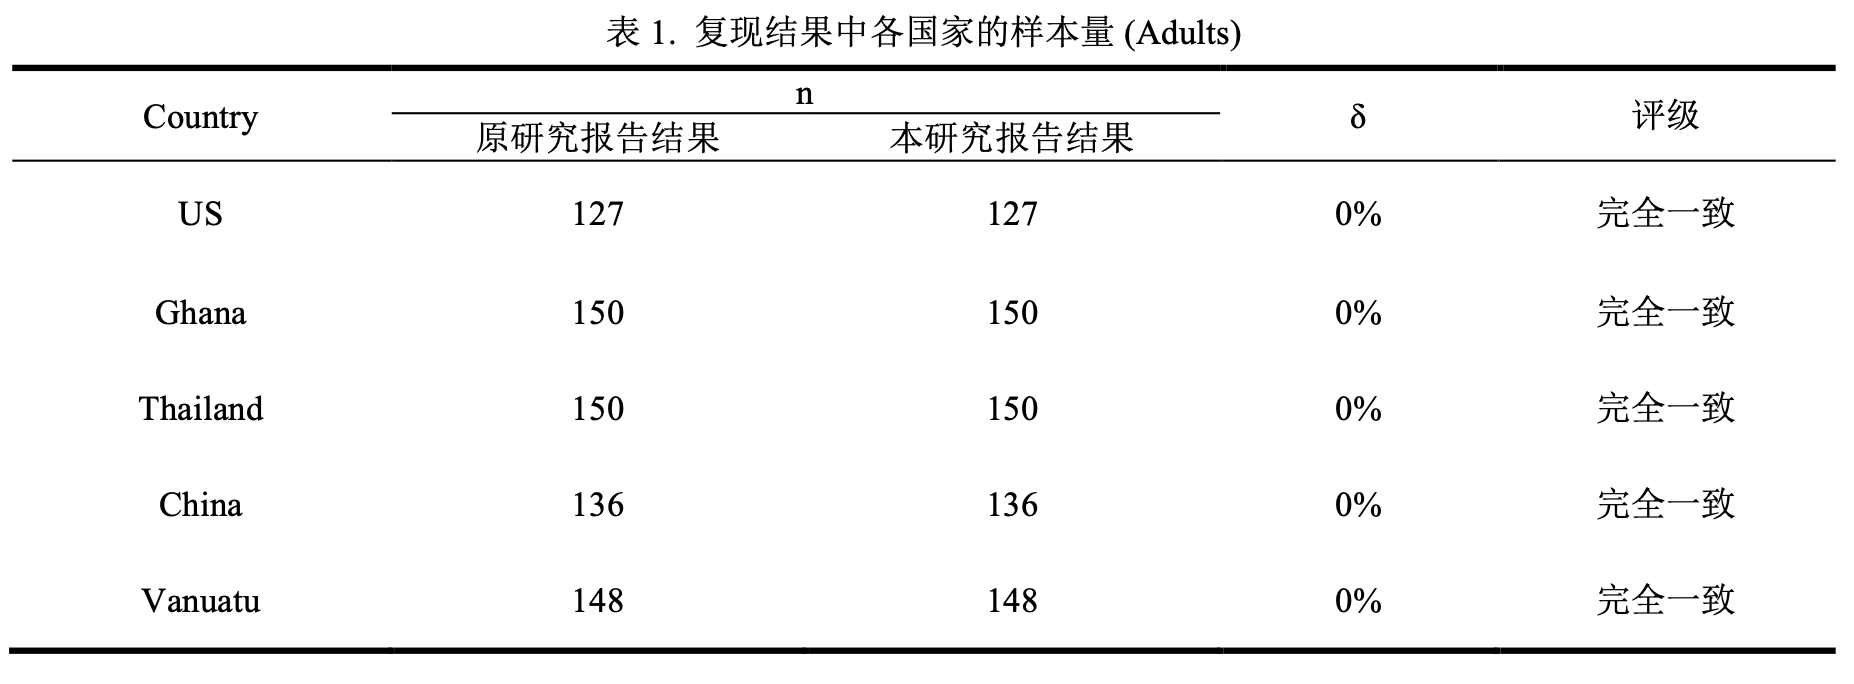
\includegraphics{./Script_Re_Weisman_2021_Group1_2024_files/Repeatability_figures/table1.png}
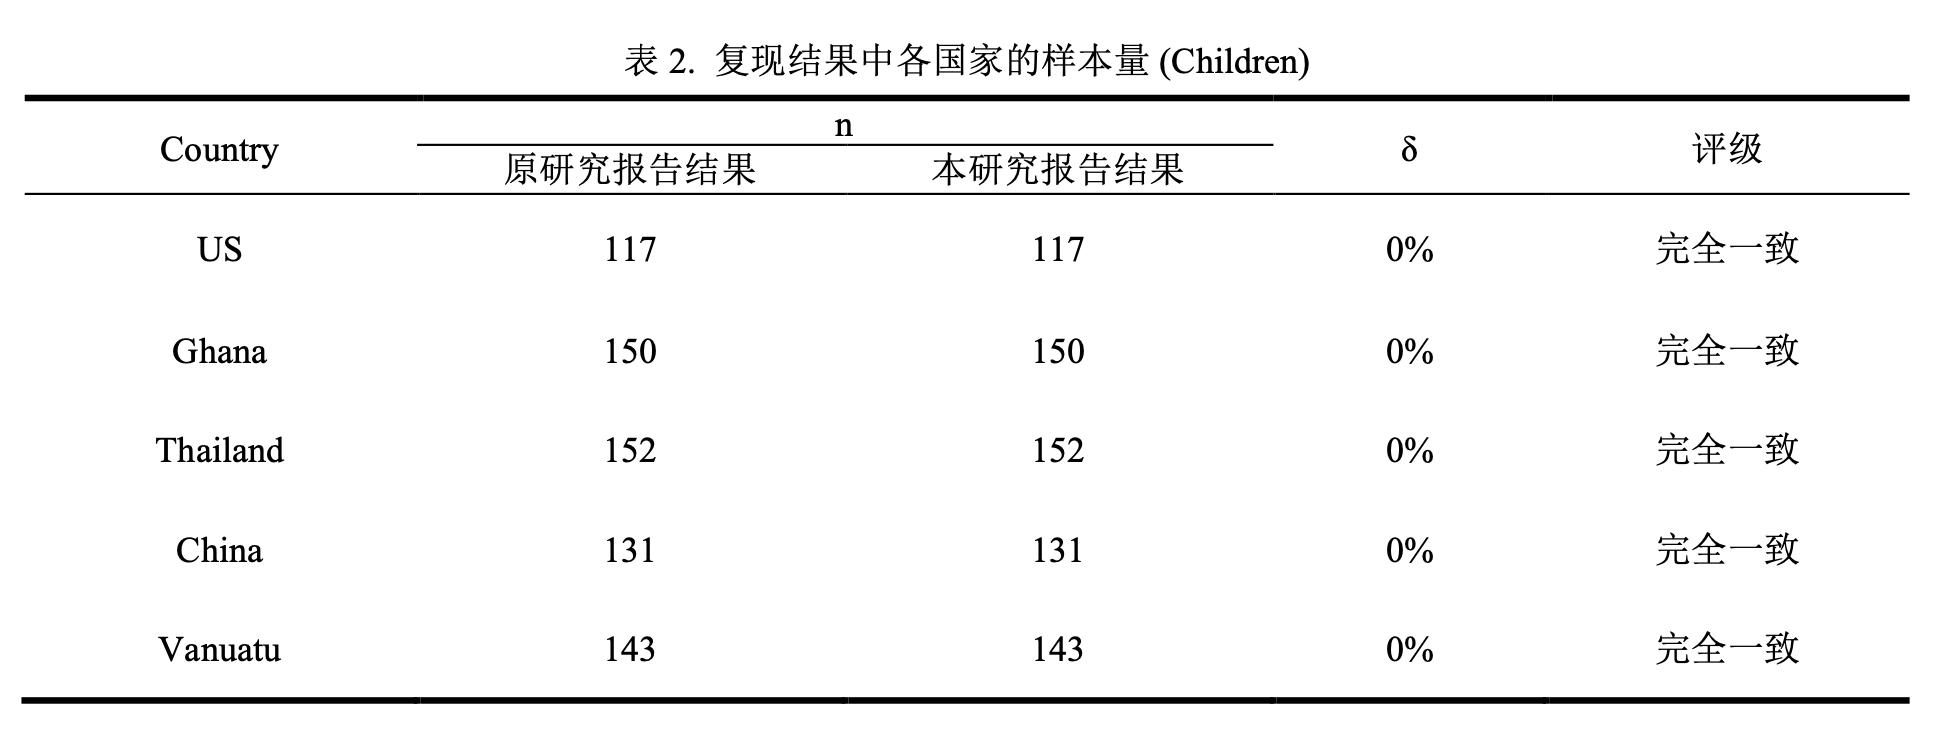
\includegraphics{./Script_Re_Weisman_2021_Group1_2024_files/Repeatability_figures/table2.png}
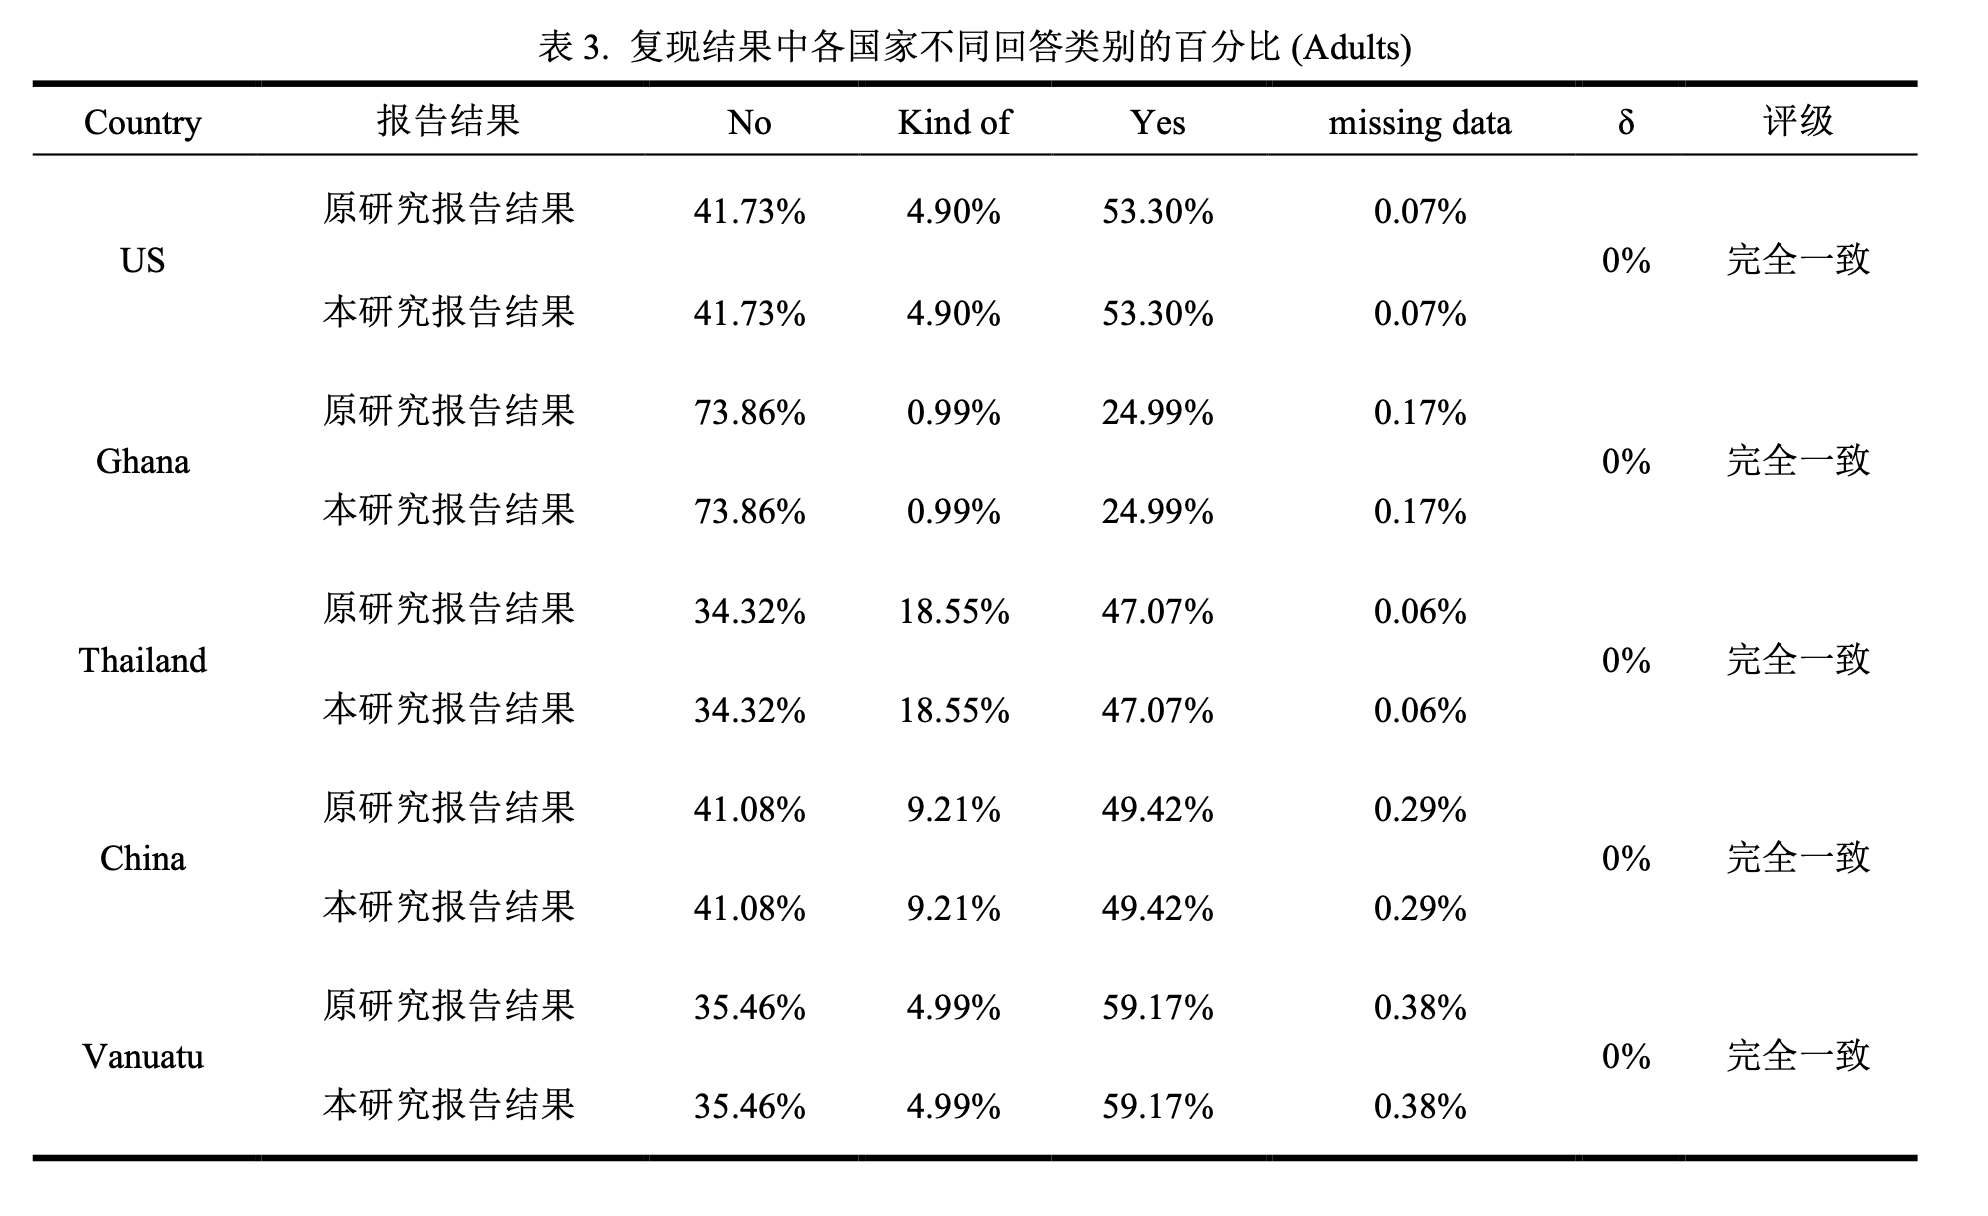
\includegraphics{./Script_Re_Weisman_2021_Group1_2024_files/Repeatability_figures/table3.png}
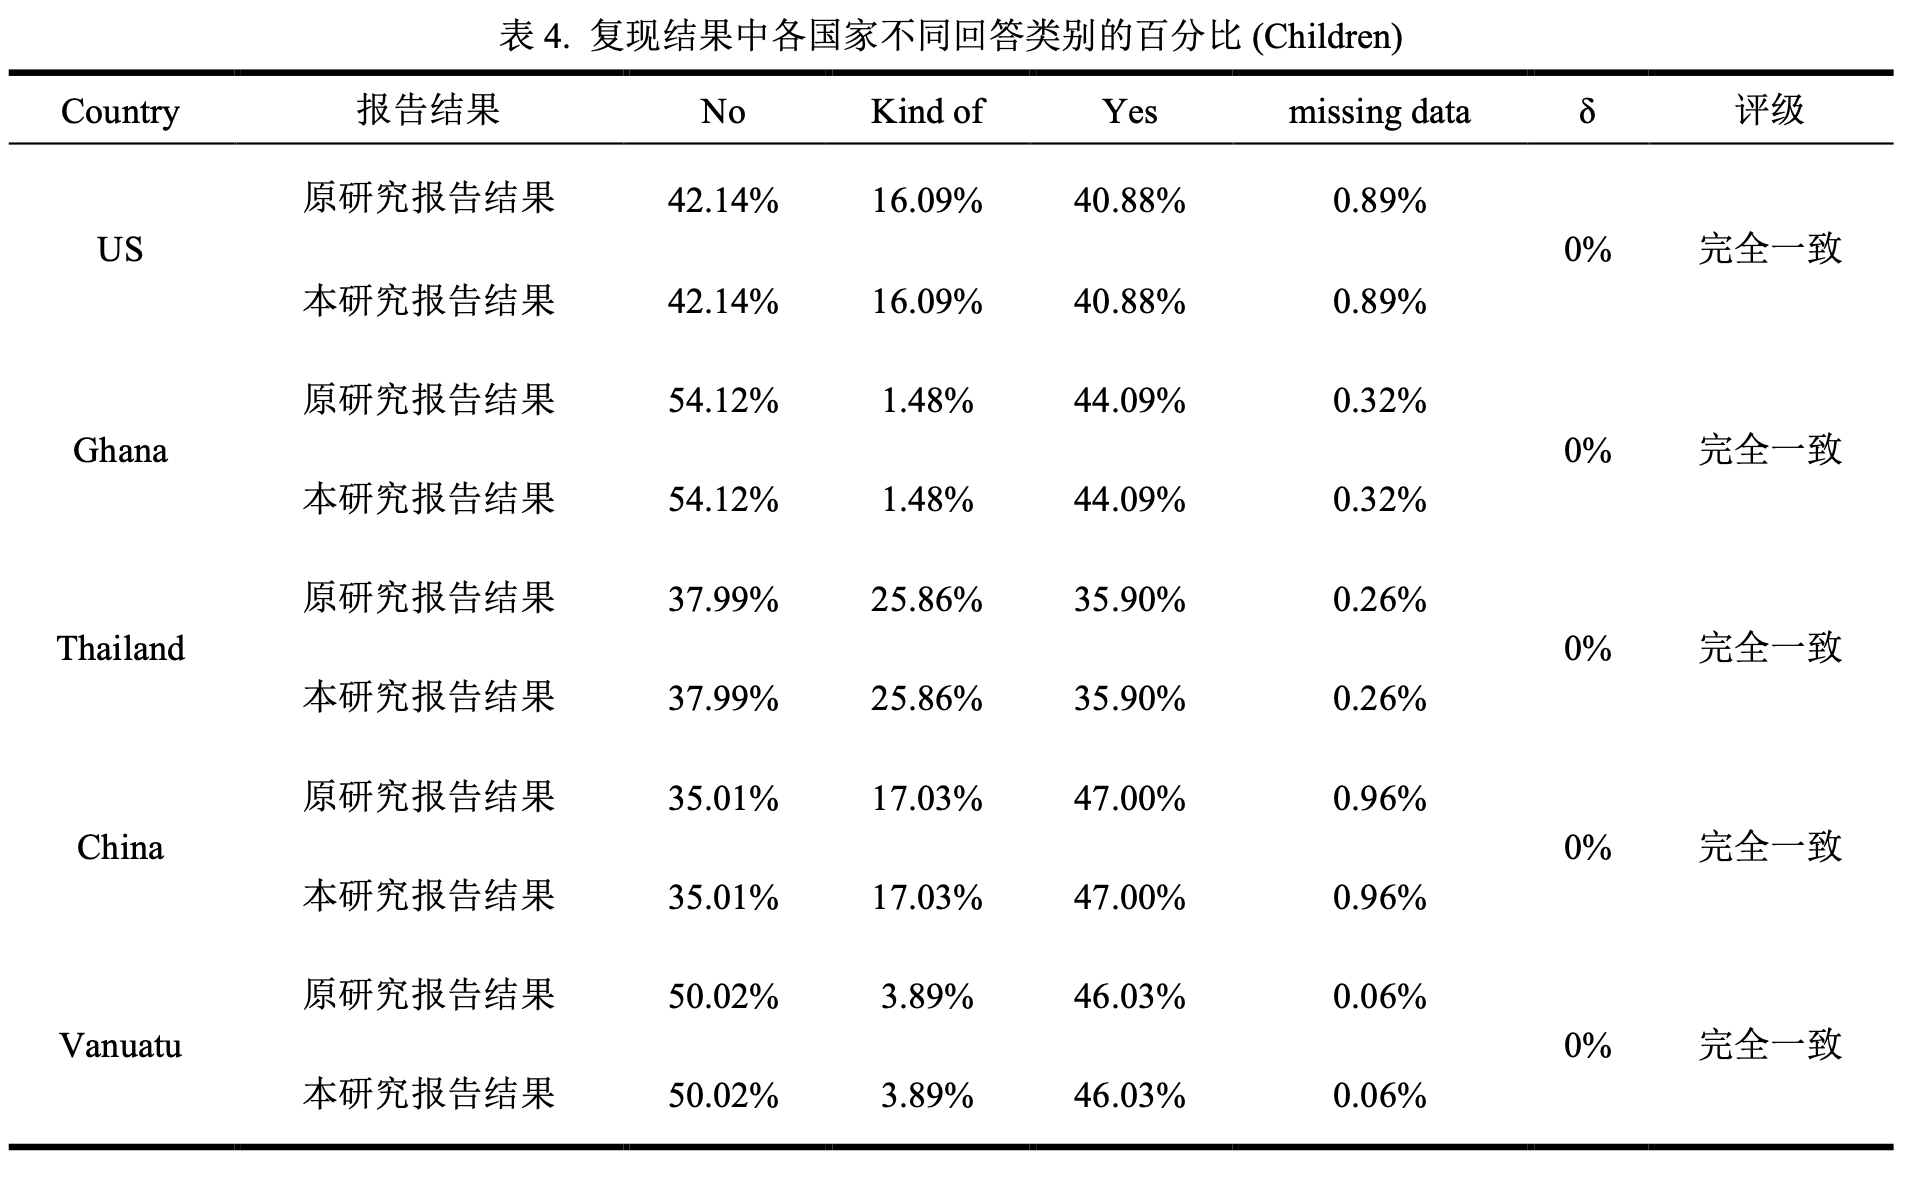
\includegraphics{./Script_Re_Weisman_2021_Group1_2024_files/Repeatability_figures/table4.png}
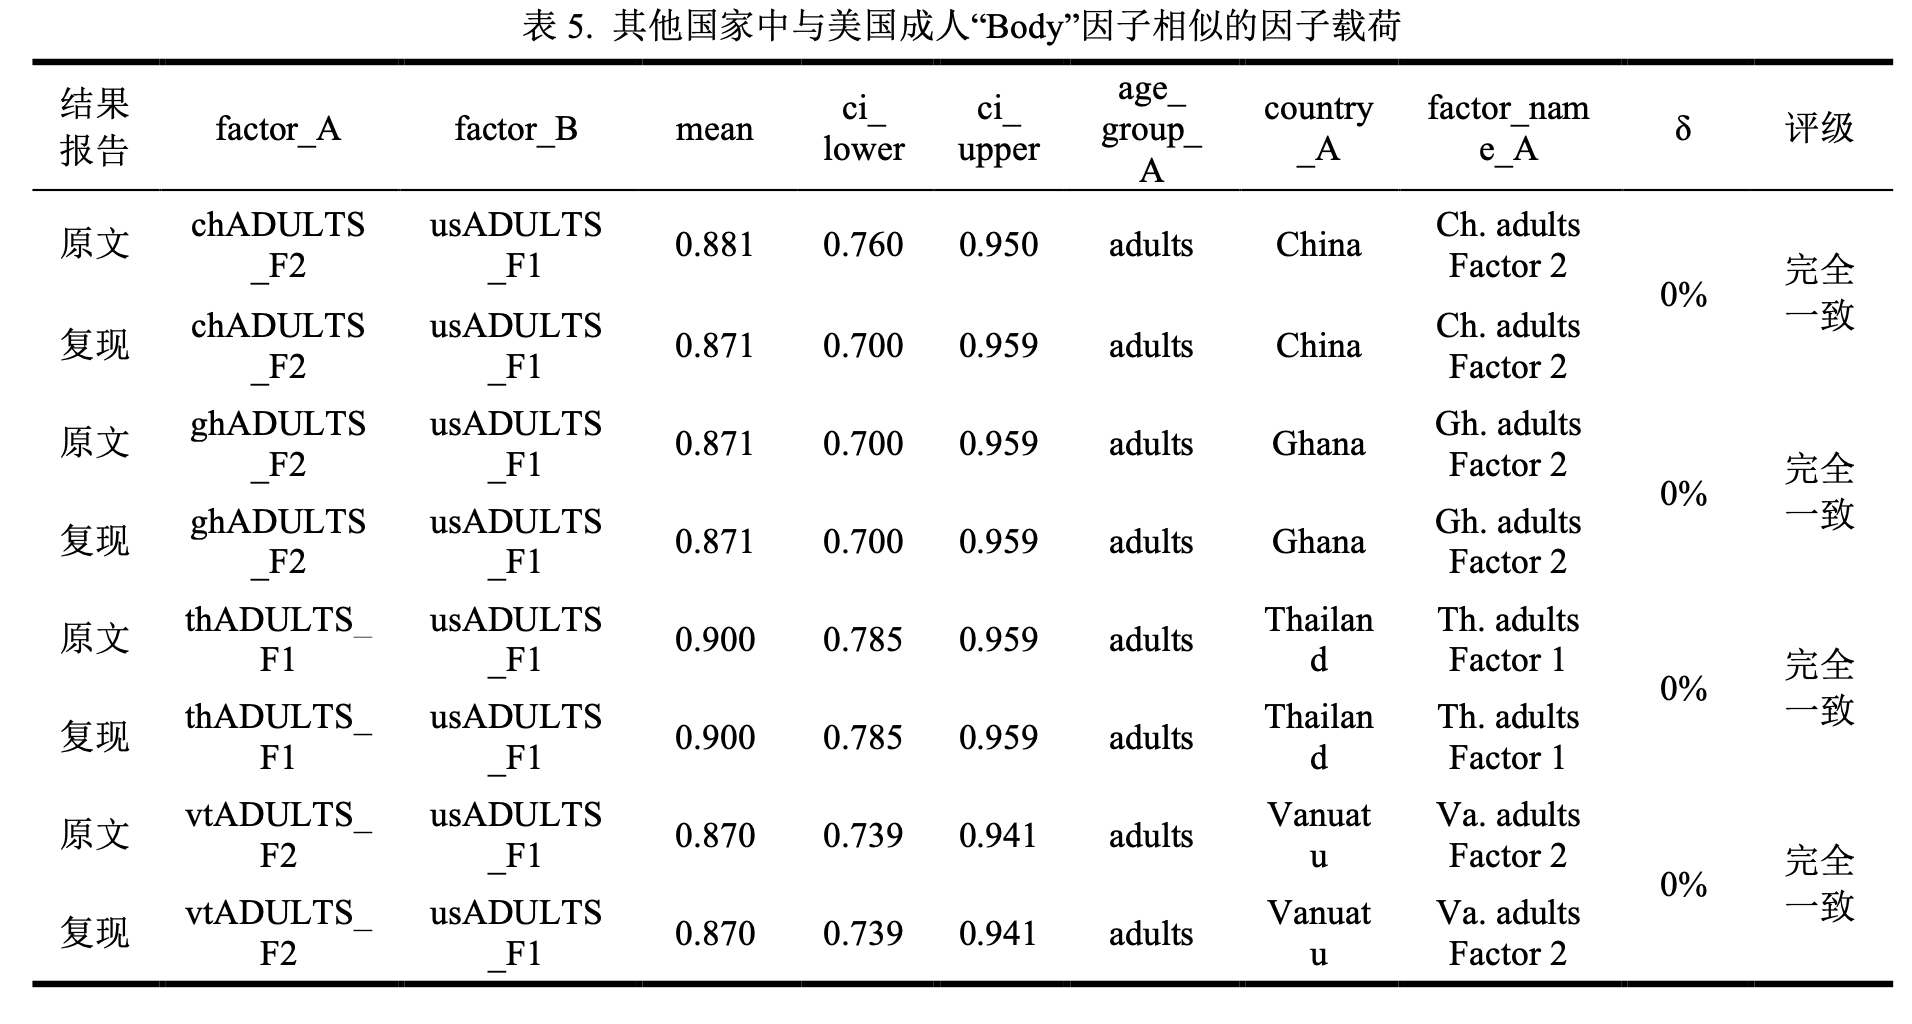
\includegraphics{./Script_Re_Weisman_2021_Group1_2024_files/Repeatability_figures/table5.png}
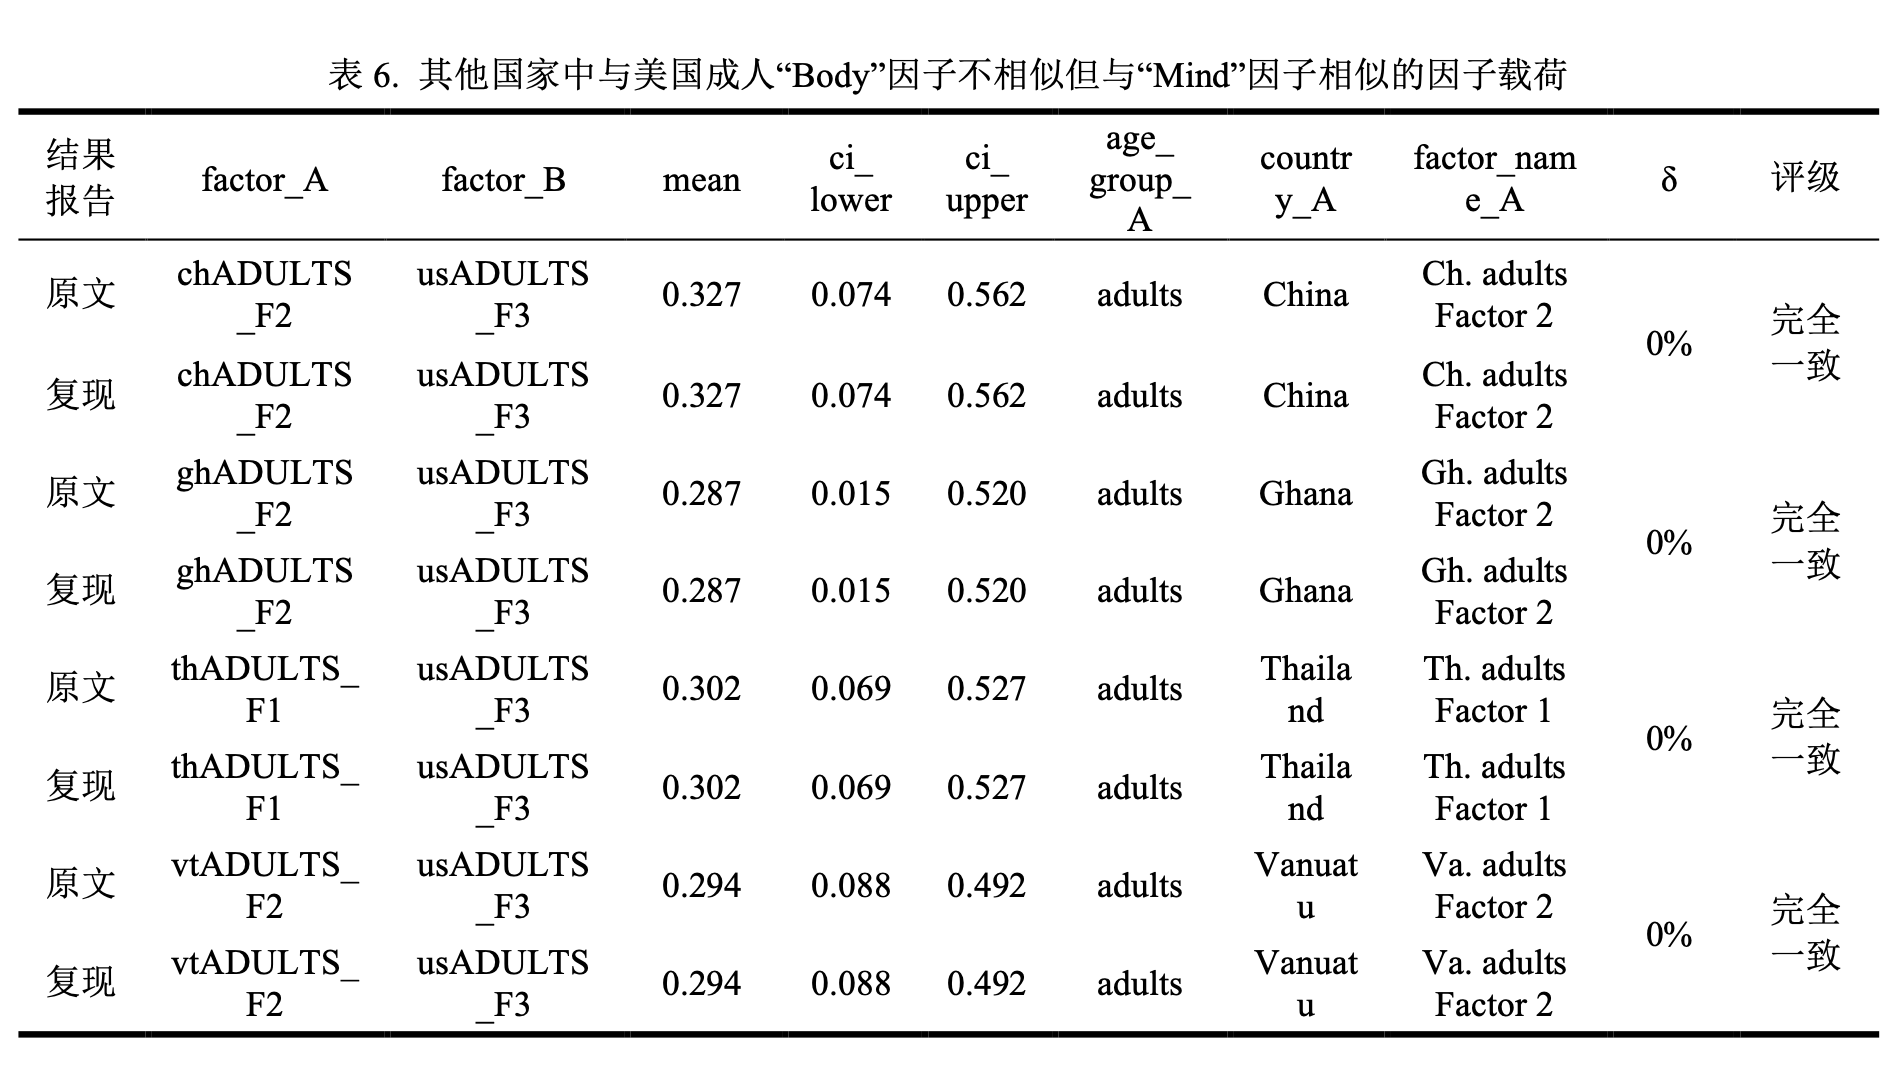
\includegraphics{./Script_Re_Weisman_2021_Group1_2024_files/Repeatability_figures/table6.png}
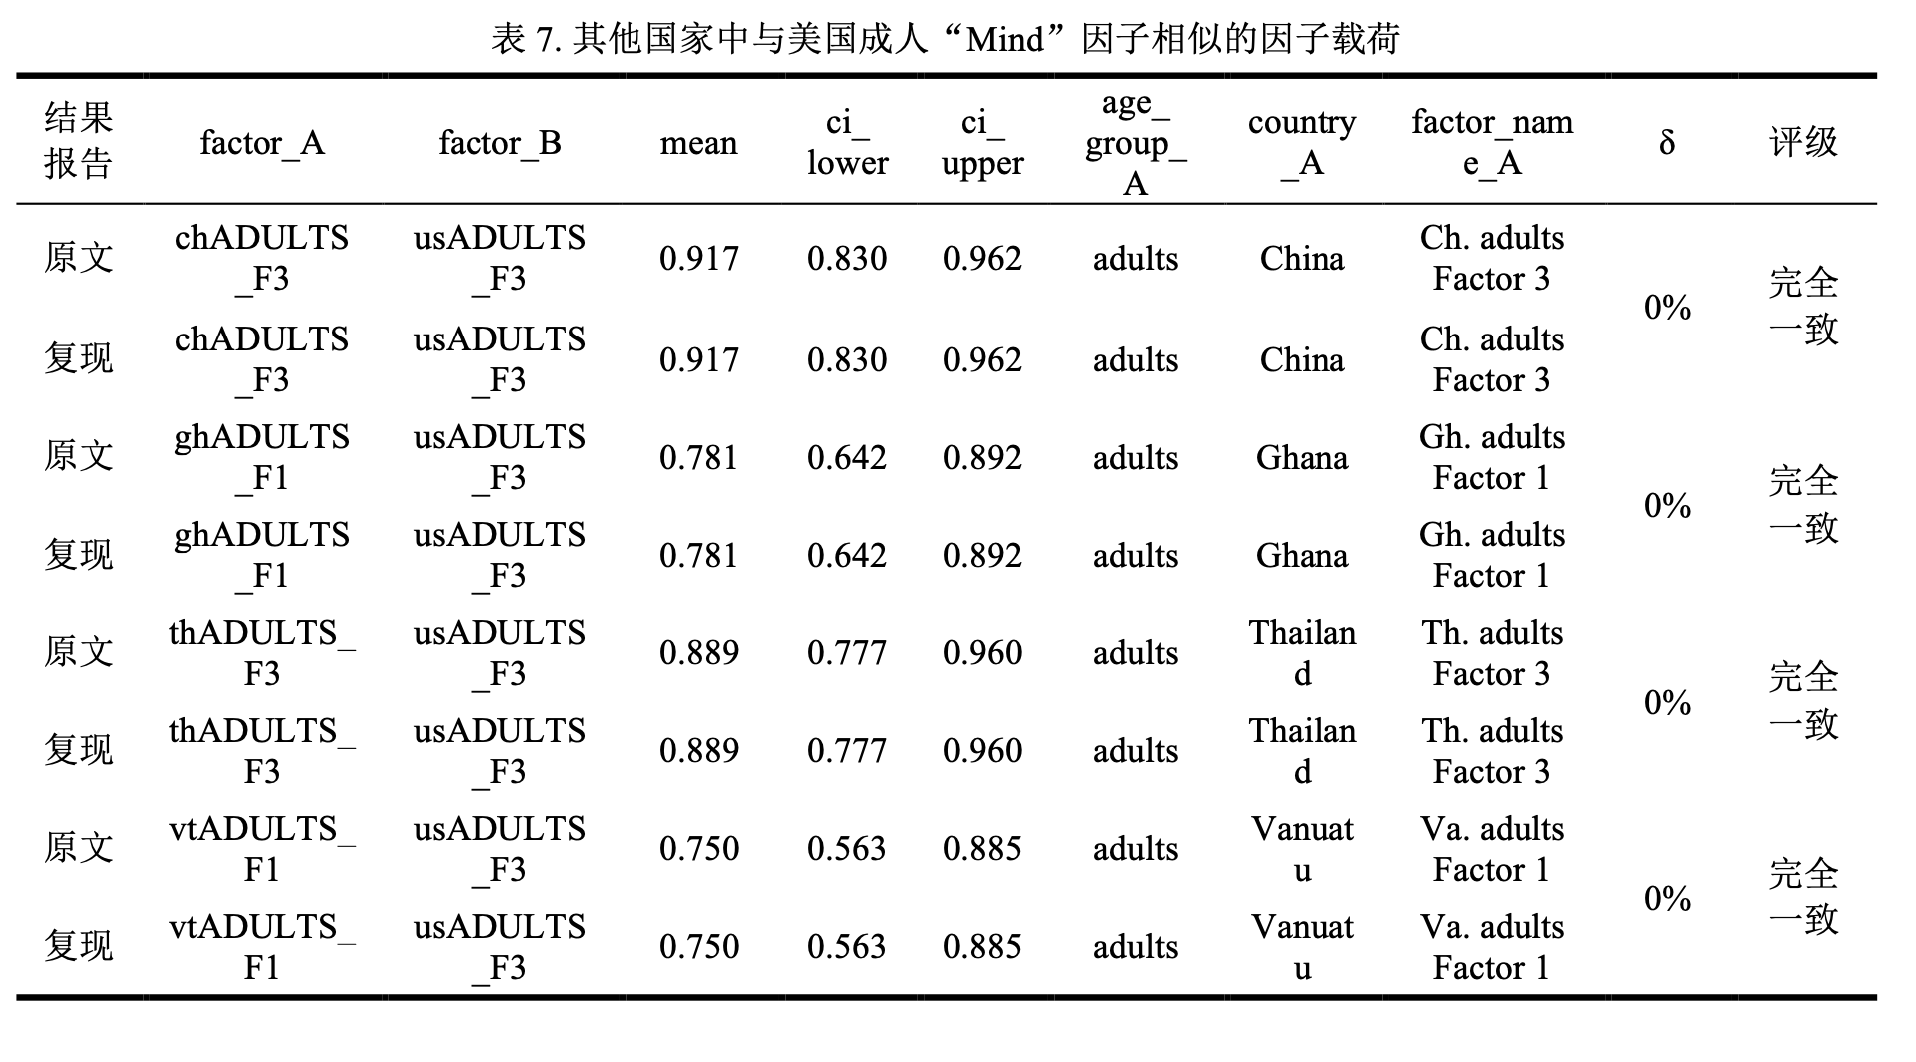
\includegraphics{./Script_Re_Weisman_2021_Group1_2024_files/Repeatability_figures/table7.png}
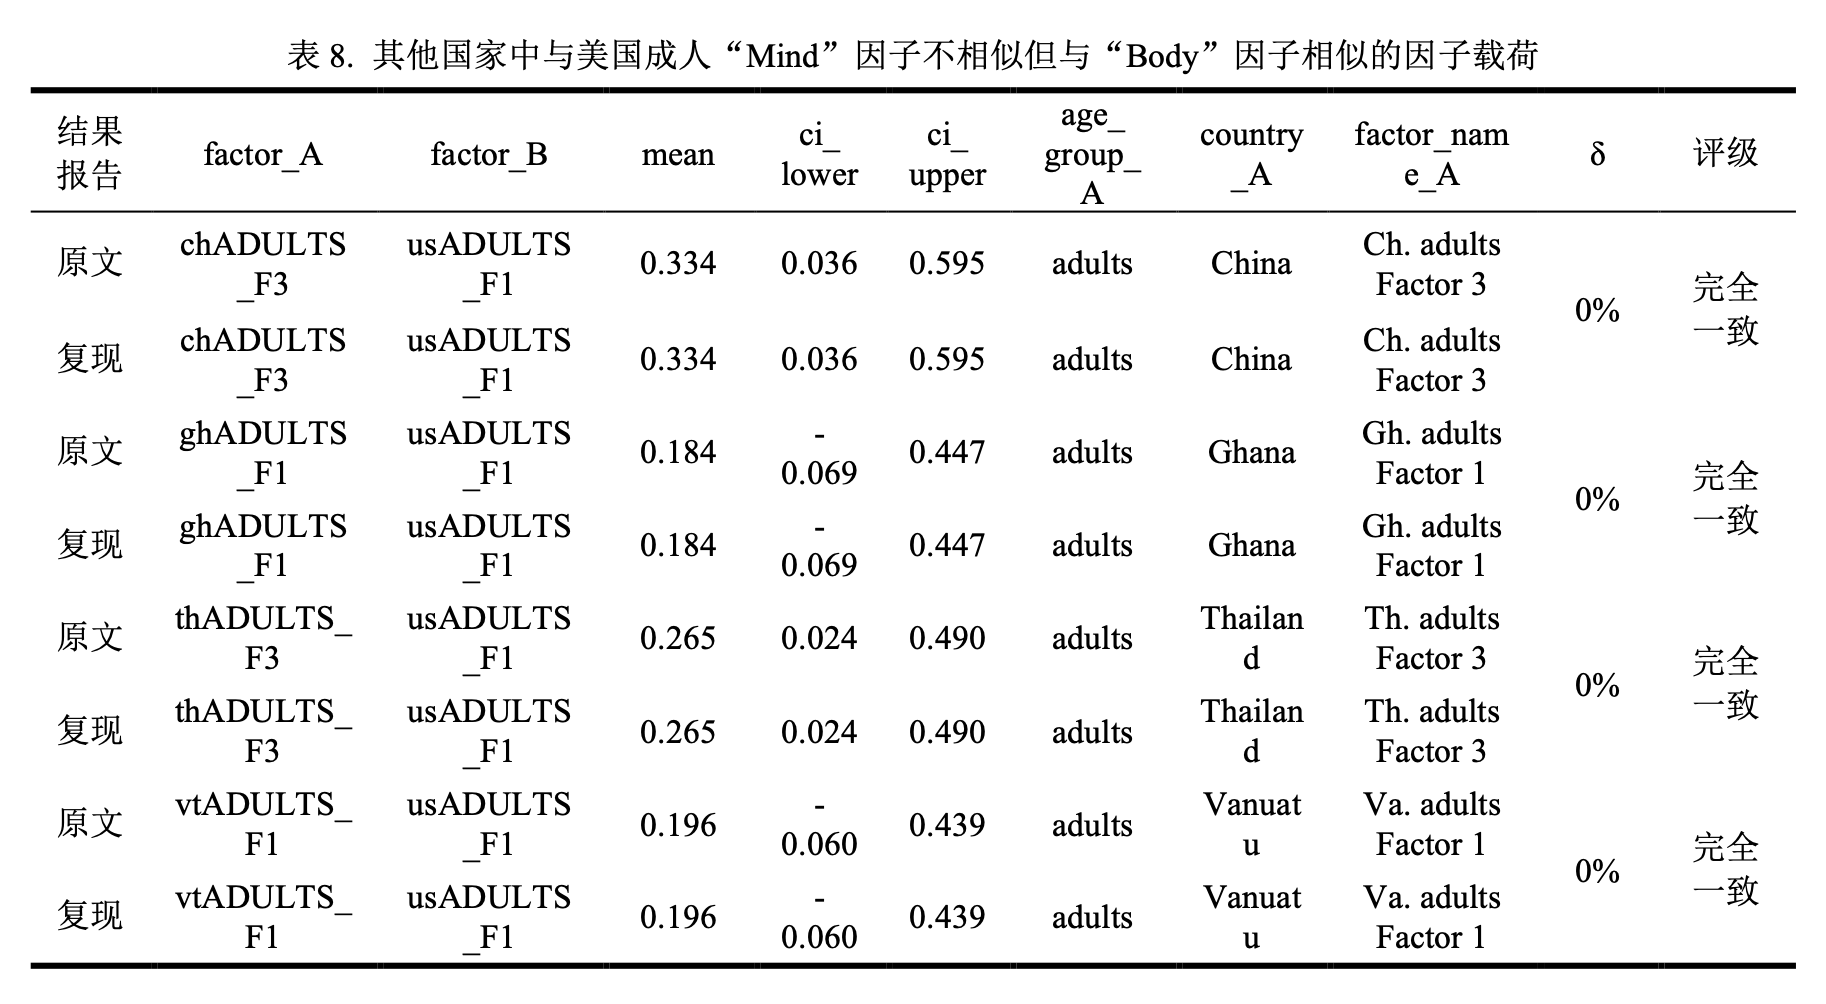
\includegraphics{./Script_Re_Weisman_2021_Group1_2024_files/Repeatability_figures/table8.png}
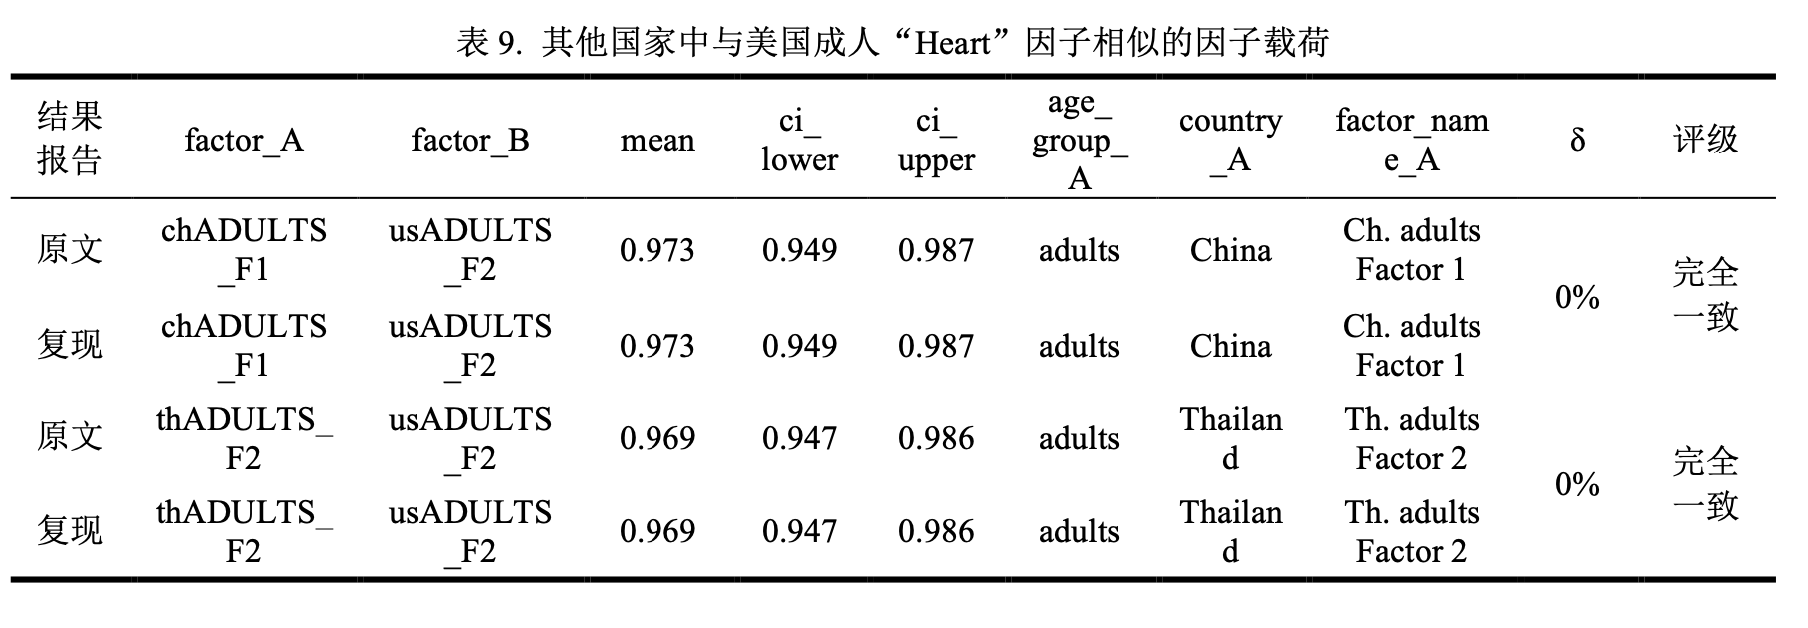
\includegraphics{./Script_Re_Weisman_2021_Group1_2024_files/Repeatability_figures/table9.png}
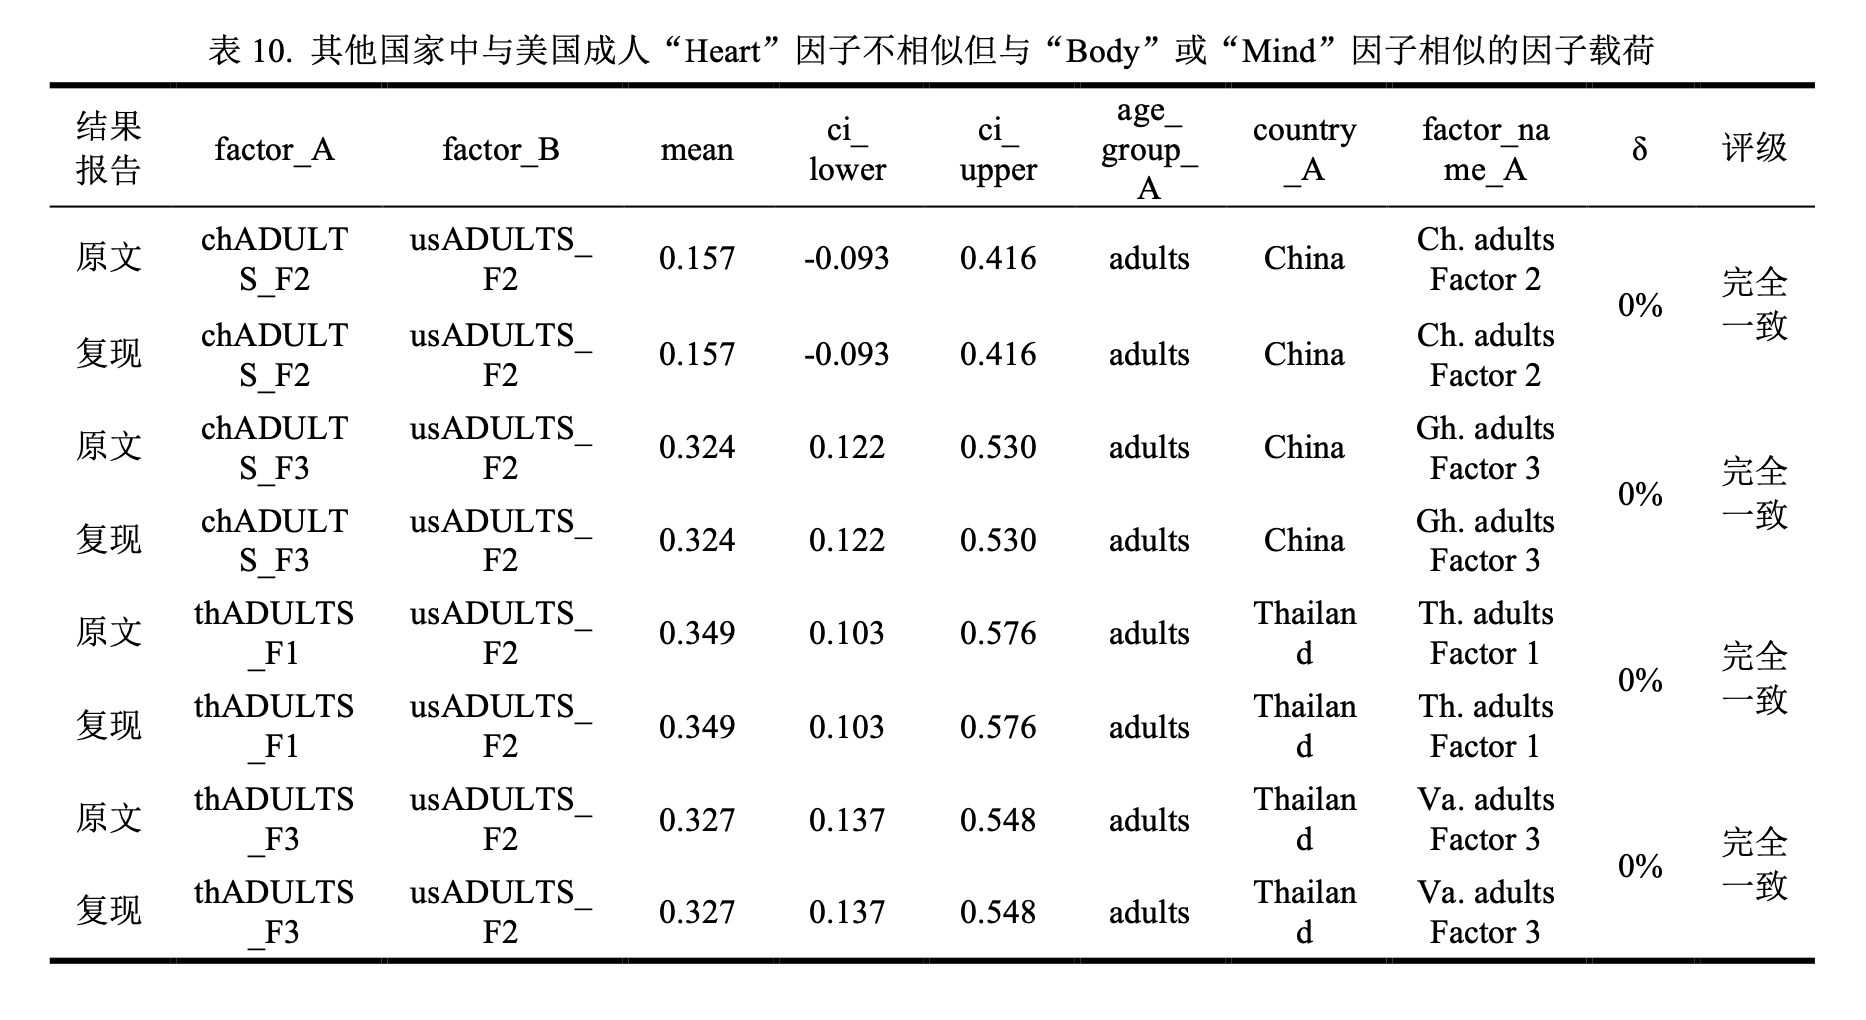
\includegraphics{./Script_Re_Weisman_2021_Group1_2024_files/Repeatability_figures/table10.png}
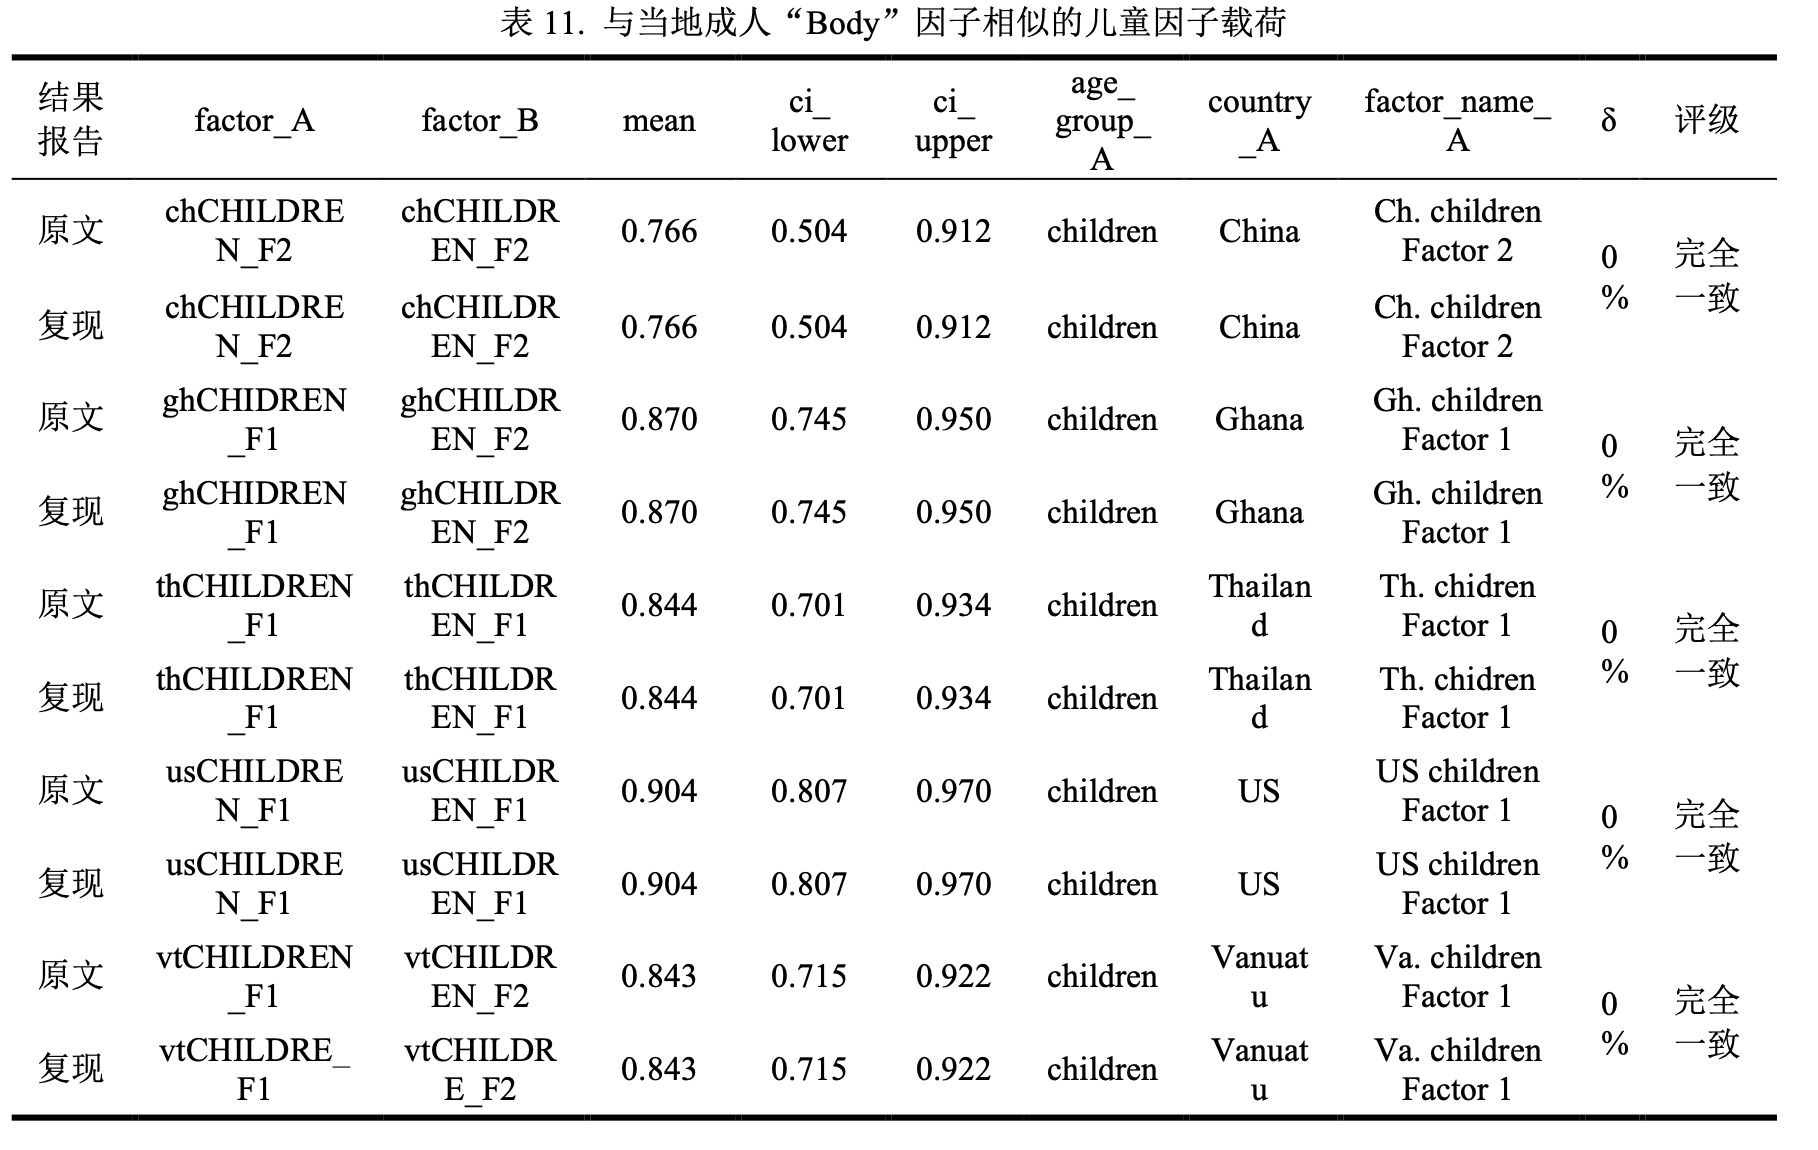
\includegraphics{./Script_Re_Weisman_2021_Group1_2024_files/Repeatability_figures/table11.png}
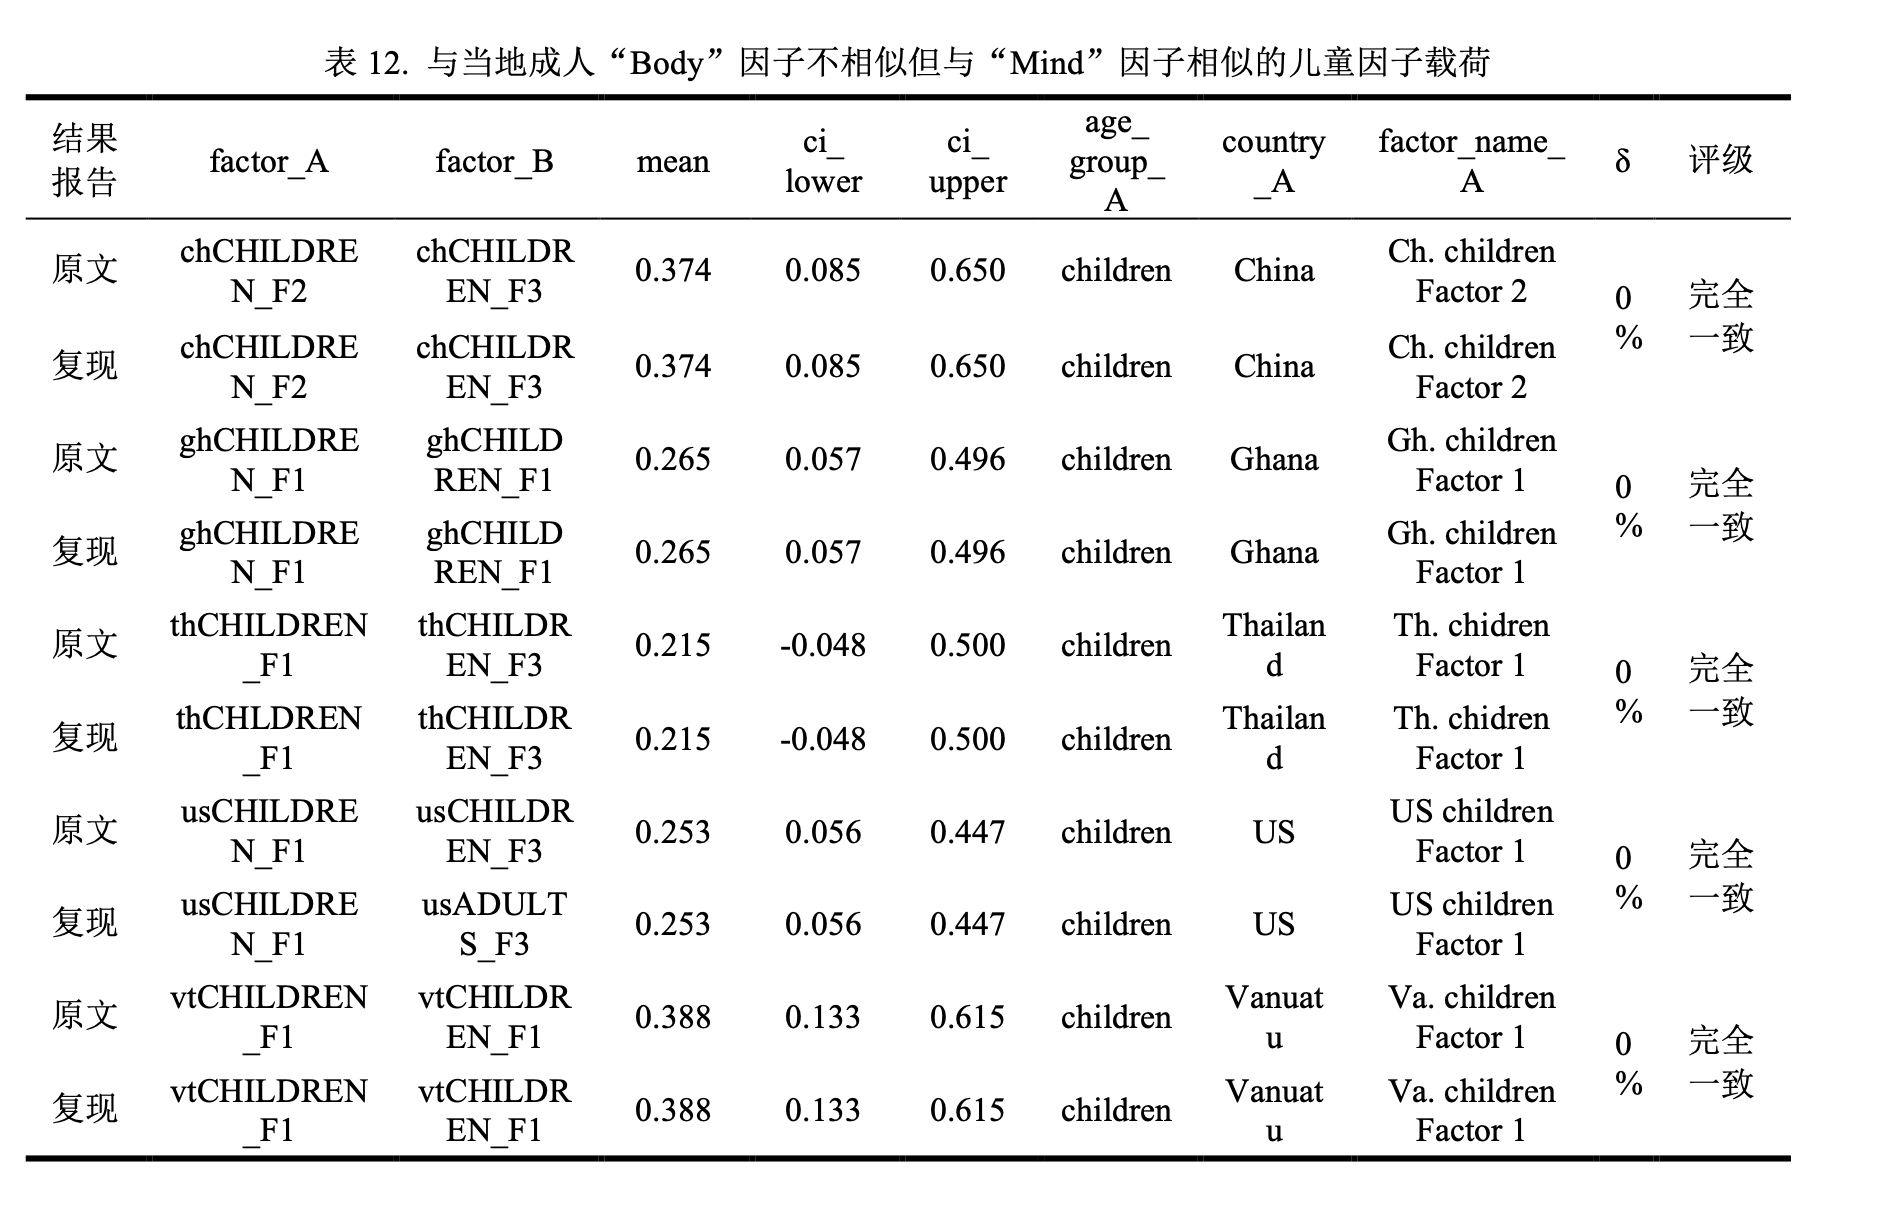
\includegraphics{./Script_Re_Weisman_2021_Group1_2024_files/Repeatability_figures/table12.png}
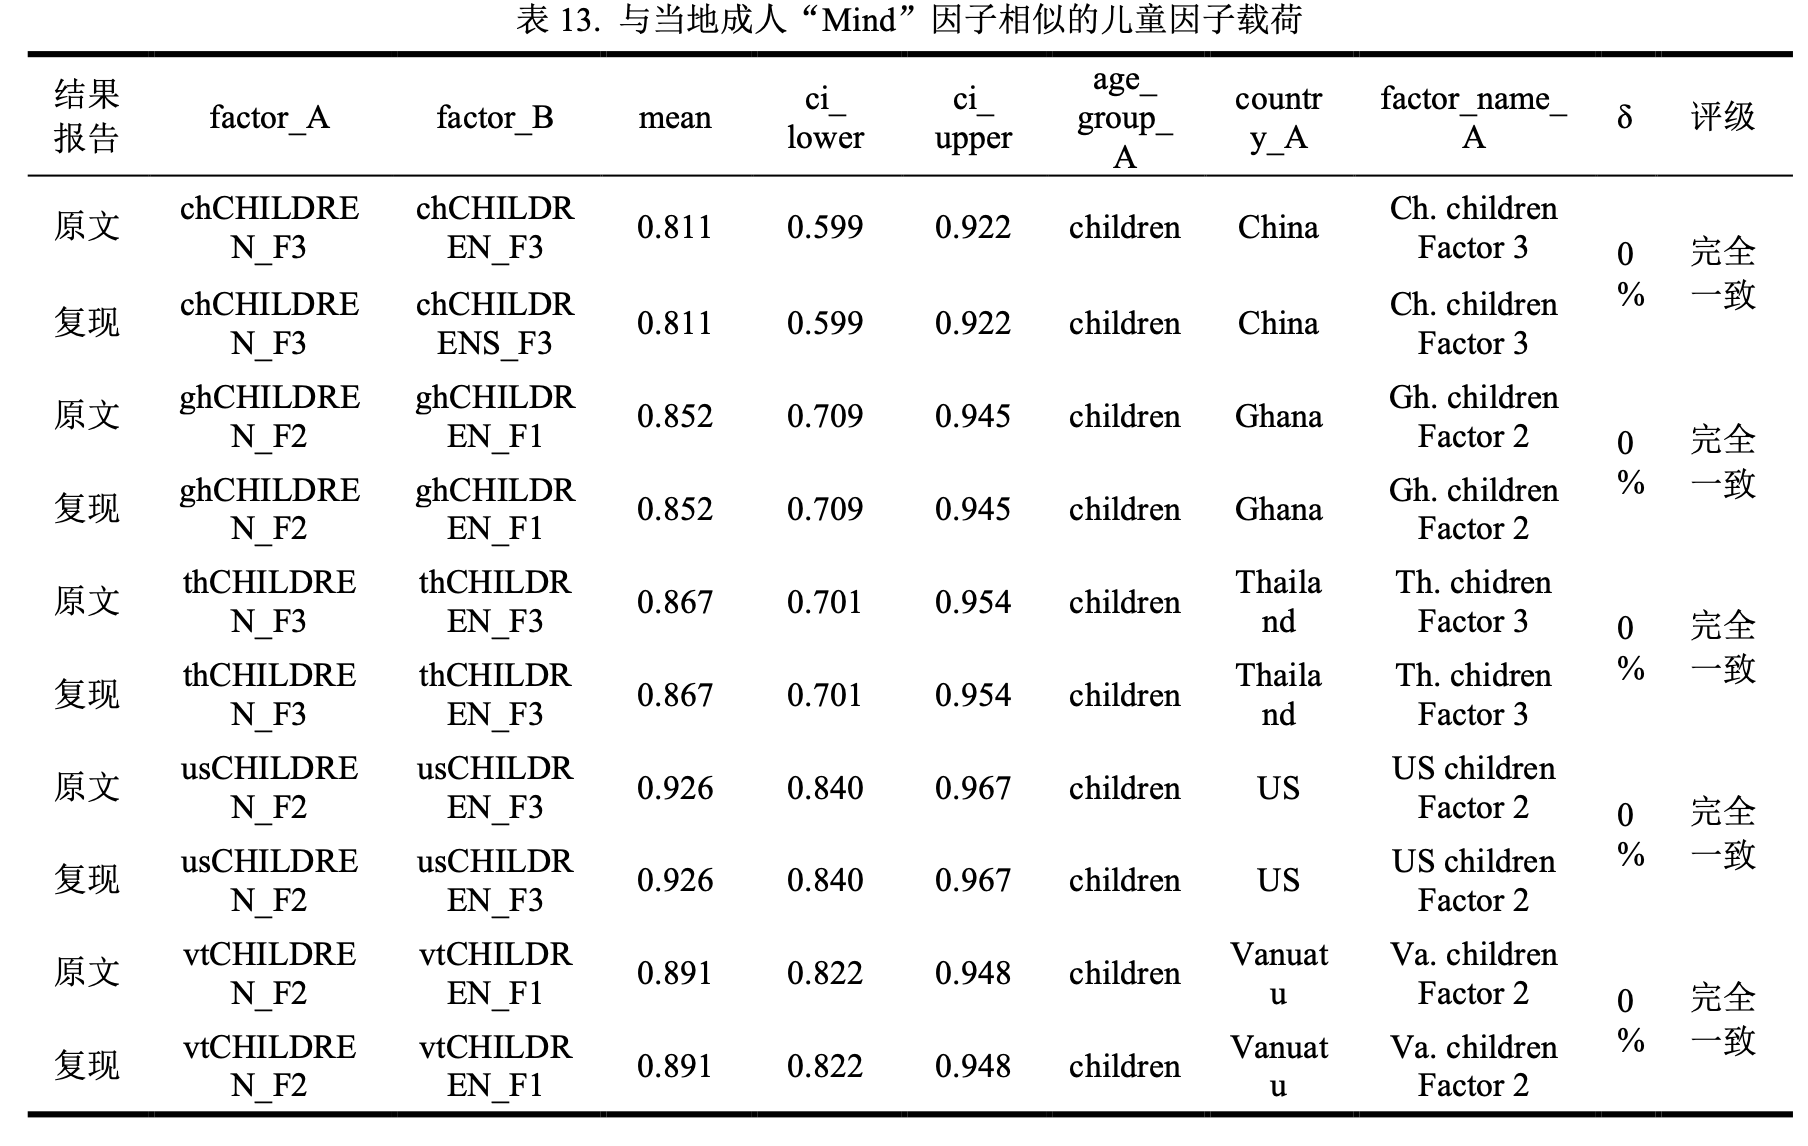
\includegraphics{./Script_Re_Weisman_2021_Group1_2024_files/Repeatability_figures/table13.png}
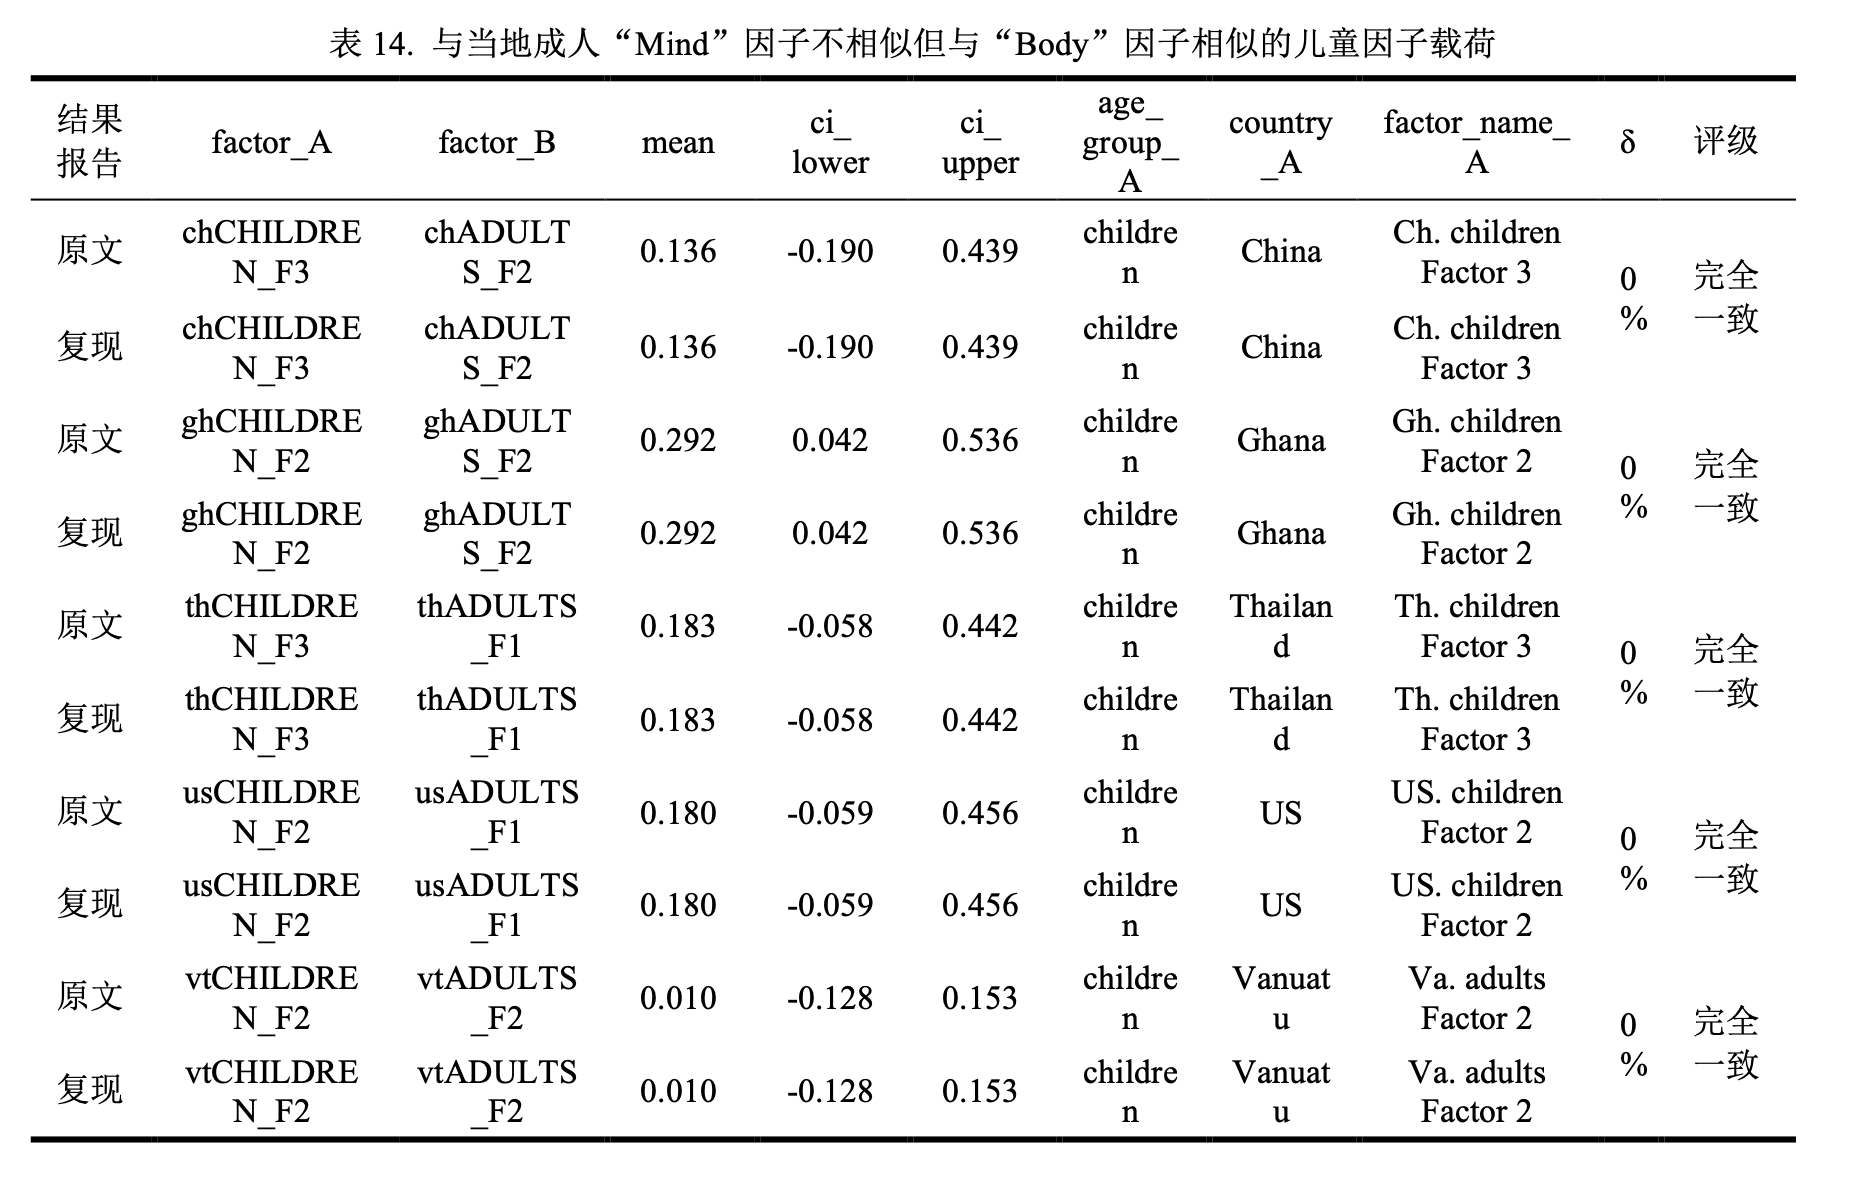
\includegraphics{./Script_Re_Weisman_2021_Group1_2024_files/Repeatability_figures/table14.png}
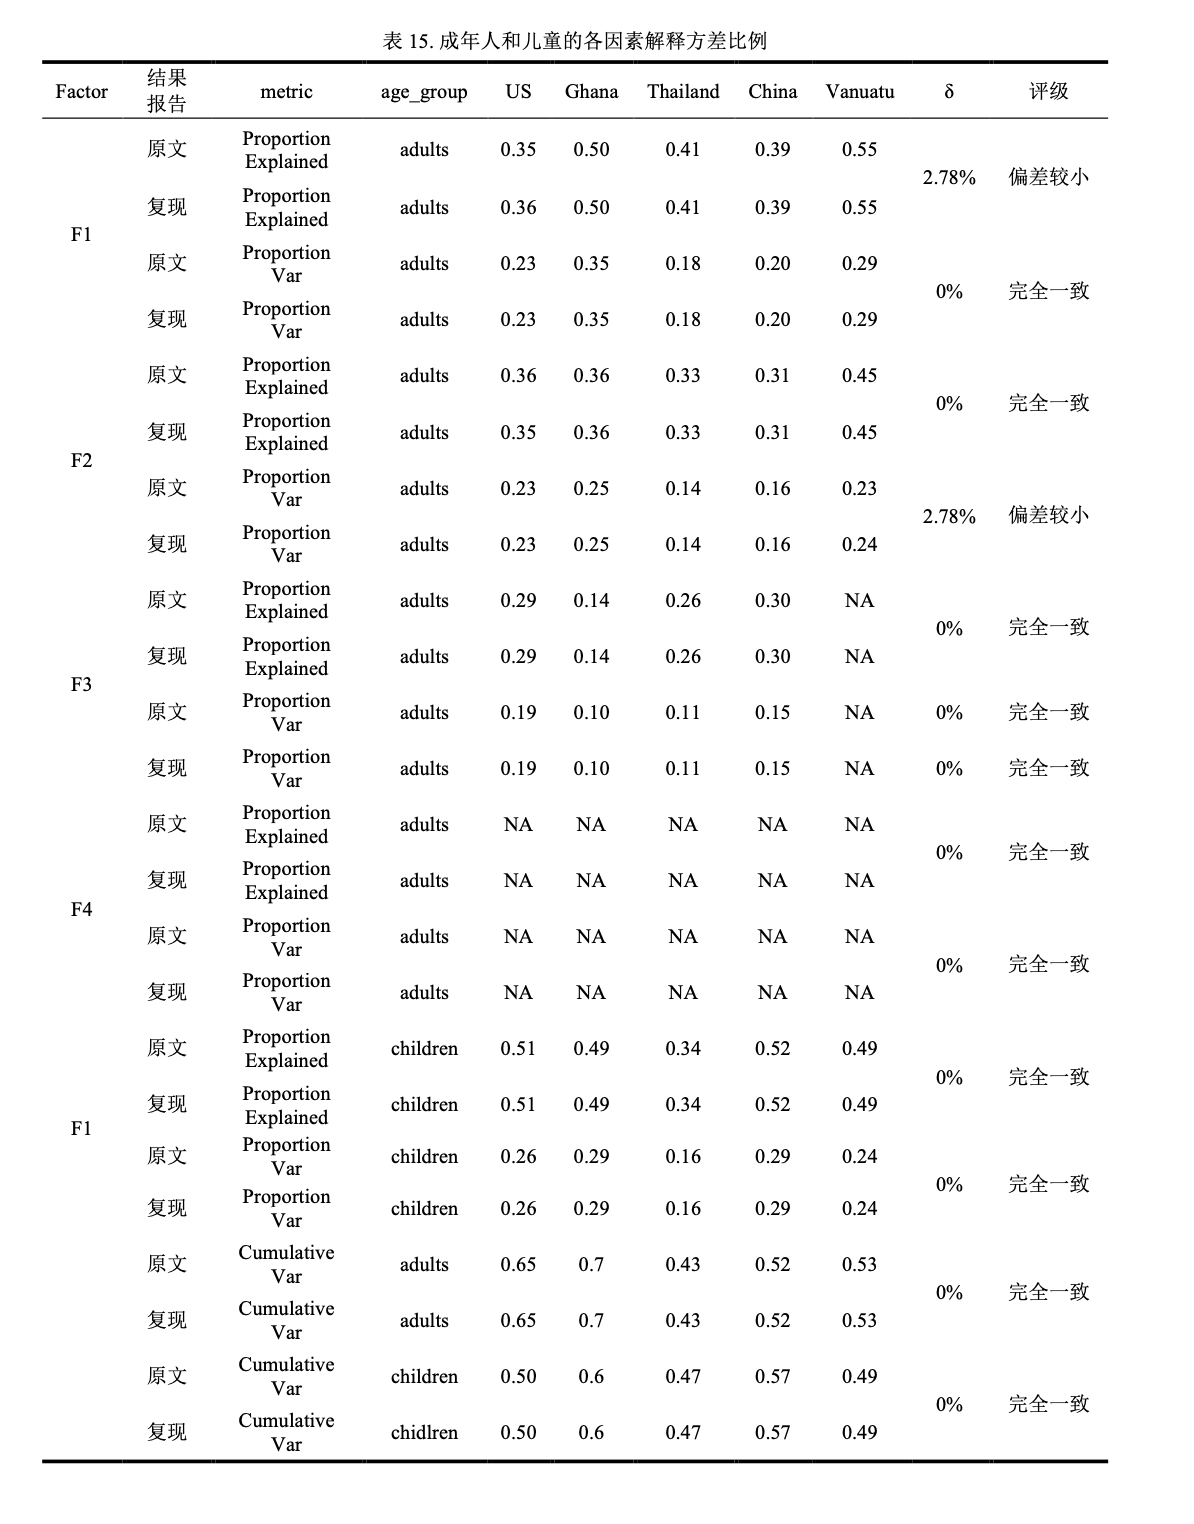
\includegraphics{./Script_Re_Weisman_2021_Group1_2024_files/Repeatability_figures/table15.png}
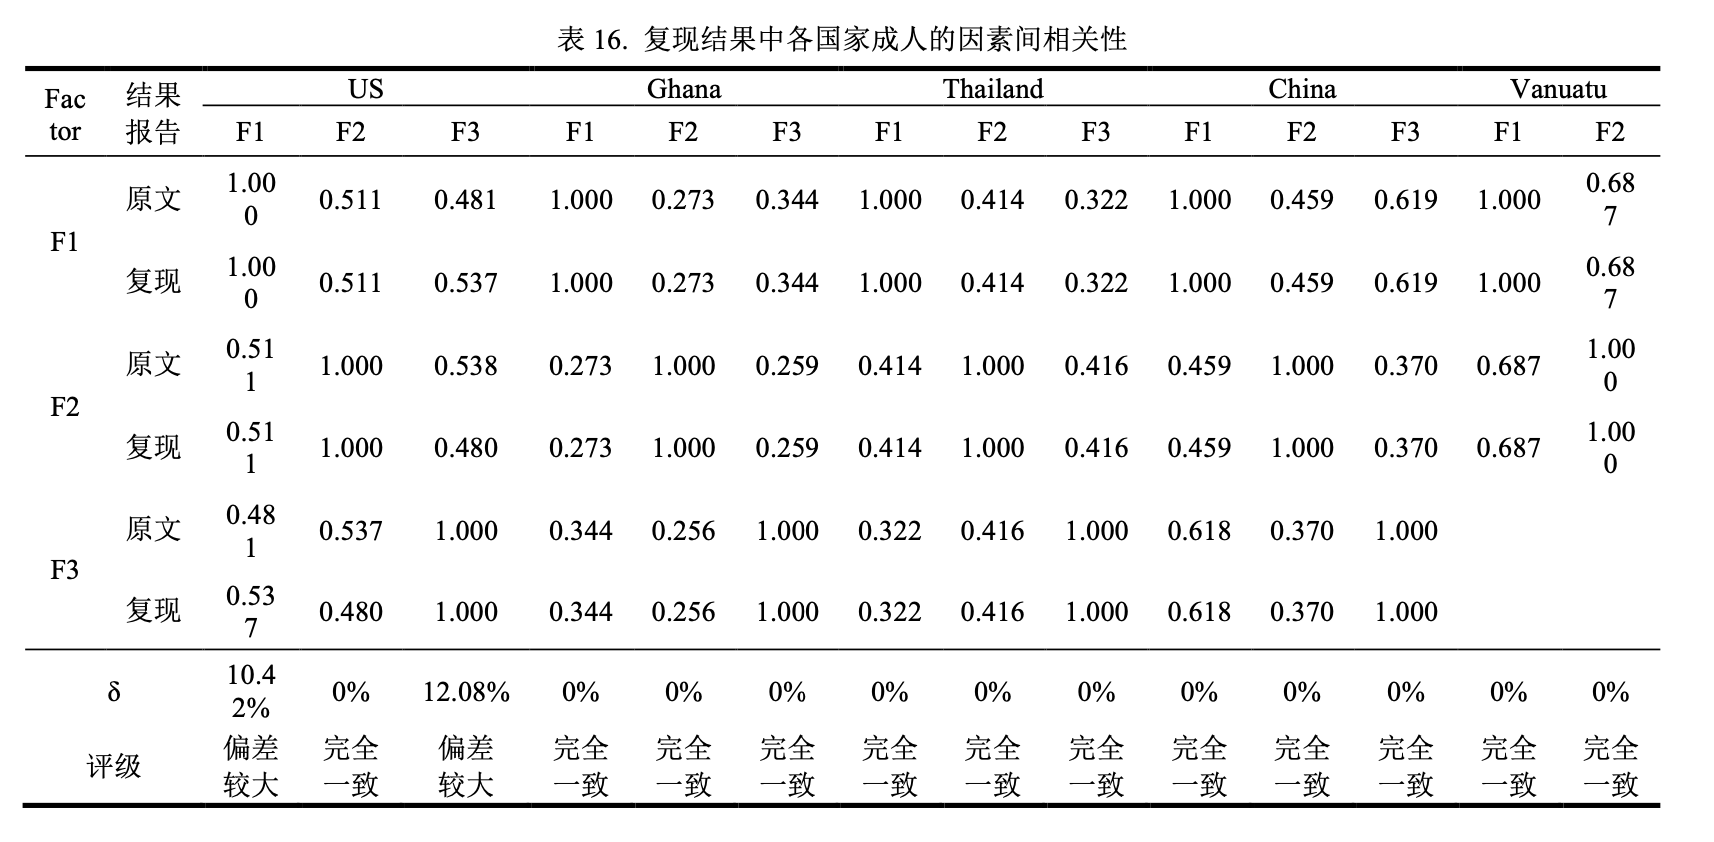
\includegraphics{./Script_Re_Weisman_2021_Group1_2024_files/Repeatability_figures/table16.png}
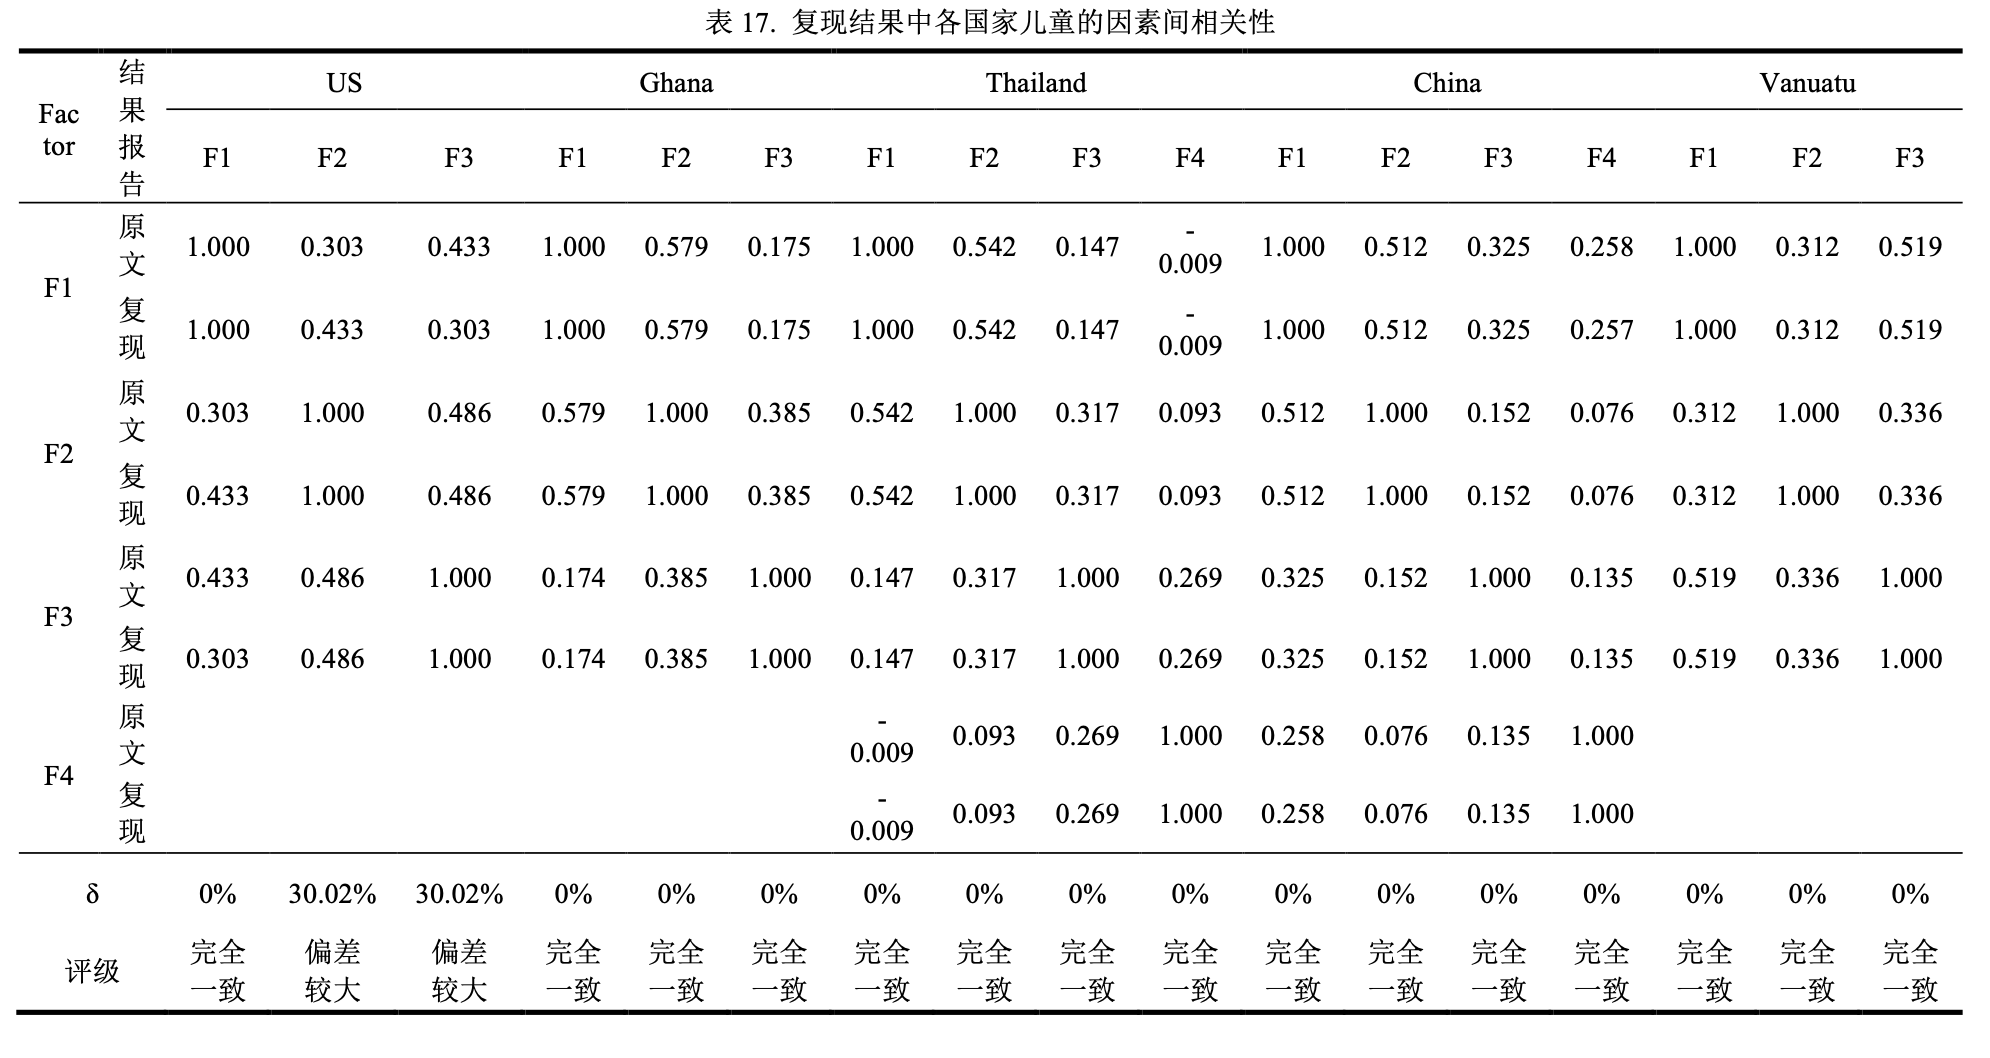
\includegraphics{./Script_Re_Weisman_2021_Group1_2024_files/Repeatability_figures/table17.png}
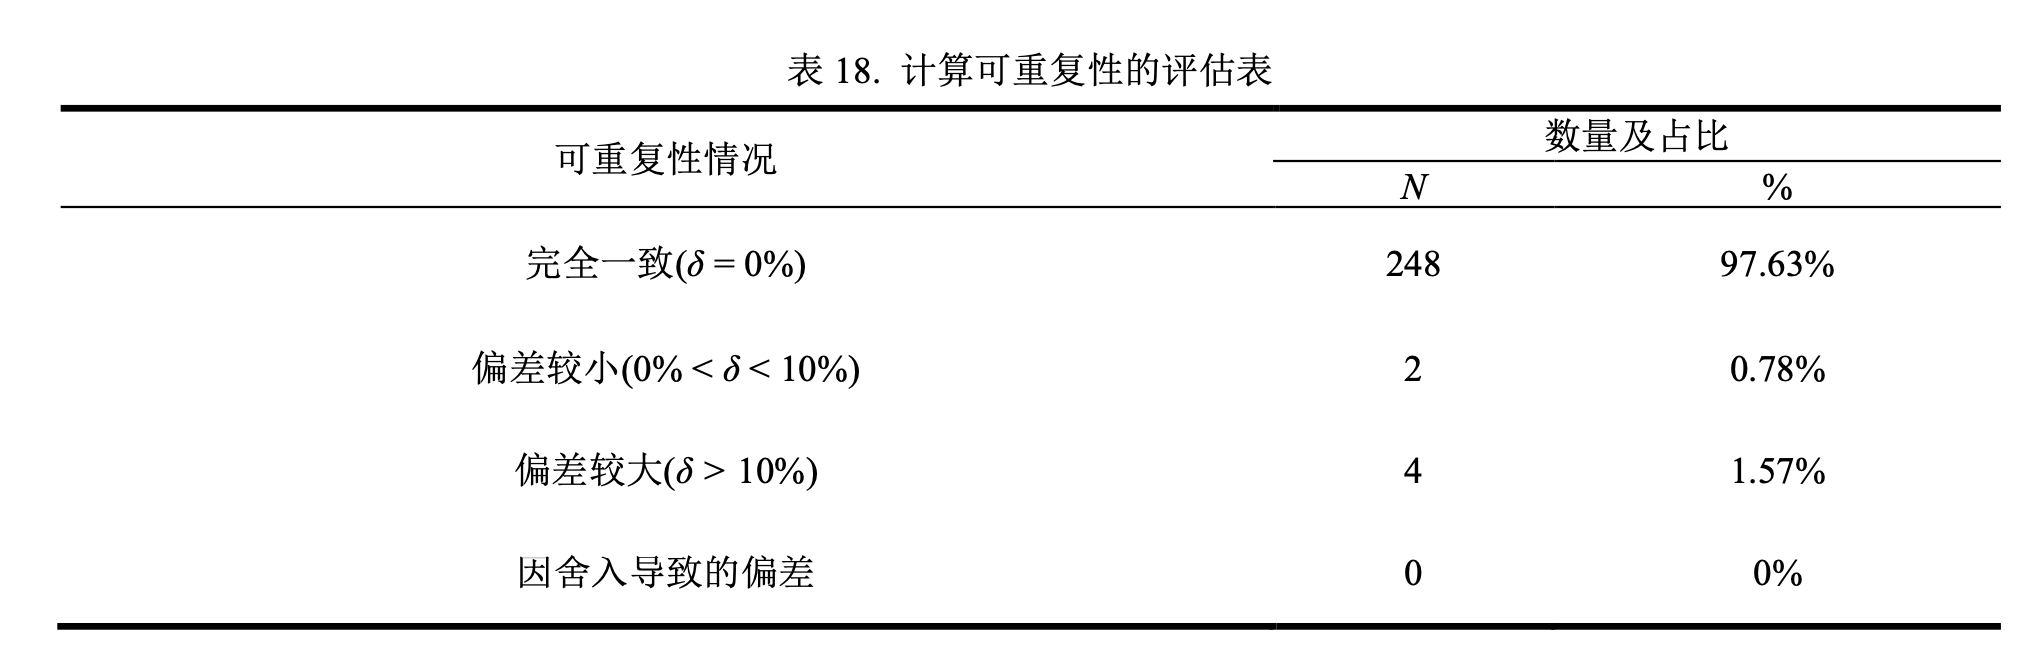
\includegraphics{./Script_Re_Weisman_2021_Group1_2024_files/Repeatability_figures/table18.png}

\hypertarget{summary-of-replication-experience}{%
\subsection{4.2 Summary of replication experience}\label{summary-of-replication-experience}}

The members of this group have also learned a lot through the reproduction of the data code in Weisman et al.'s paper, and based on their sharing, this section will summarize the key points of everyone's experience and experience:

\begin{enumerate}
\def\labelenumi{\arabic{enumi}.}
\tightlist
\item
  \textbf{Understanding Code Overview}:

  \begin{itemize}
  \tightlist
  \item
    Avoid using the \texttt{source()} function in R Markdown to prevent automatic execution of loaded R scripts. Manual review of R scripts helps in comprehensively understanding the authors' data analysis approach.
  \end{itemize}
\item
  \textbf{Distinguishing \texttt{require} and \texttt{library} Functions}:

  \begin{itemize}
  \tightlist
  \item
    Use \texttt{require(package)} to return FALSE if the package is missing or fails to load, while \texttt{library(package)} halts execution if loading fails. Understanding this distinction is crucial for script continuity.
  \end{itemize}
\item
  \textbf{Custom Functions and Scripts}:

  \begin{itemize}
  \tightlist
  \item
    Authors often create custom functions in separate scripts for data processing, exploratory factor analysis, regression analysis, reliability analysis, scoring, and visualization. Enhancing code modularity and readability.
  \end{itemize}
\item
  \textbf{Data Preprocessing}:

  \begin{itemize}
  \tightlist
  \item
    Excluding specific data files or directories containing ``raw'' in their names, as indicated in the .gitignore file, is common practice. Understanding the authors' data preprocessing steps is essential for successful replication.
  \end{itemize}
\item
  \textbf{Coding Style and \texttt{\%\textgreater{}\%} Pipe Operator}:

  \begin{itemize}
  \tightlist
  \item
    Familiarize with authors' coding style, including using the \texttt{\%\textgreater{}\%} pipe operator from the dplyr package for smoother and more readable data processing. The pipe operator facilitates chaining operations and streamlines code.
  \end{itemize}
\item
  \textbf{Visualization in R Markdown}:

  \begin{itemize}
  \tightlist
  \item
    When plotting with ggplot2 in R Markdown, pay attention to saving graphs using \texttt{ggsave()} due to differences in display panes between R Markdown and R scripts.
  \end{itemize}
\item
  \textbf{Interdisciplinary Insights}:

  \begin{itemize}
  \tightlist
  \item
    Compare psychological research in the paper with the philosophical ``Three Worlds'' theory to derive insights from other disciplines. Avoid relying solely on internal disciplinary assumptions in psychological research and consider adopting bottom-up research methods, especially in fields susceptible to researcher bias.
  \end{itemize}
\item
  \textbf{R Language Learning Experience}:

  \begin{itemize}
  \tightlist
  \item
    Utilize forums, university websites, and other resources to deepen understanding of unfamiliar terms, theoretical concepts, and analytical tools' usage, while staying updated on subject-specific research group discussions.
  \end{itemize}
\item
  \textbf{PPT Design and Presentation Skills}:

  \begin{itemize}
  \tightlist
  \item
    Emphasize concise and information-rich PPT design with logical coherence and clear structure. Avoid excessive text and prioritize the use of images for effective information presentation.
  \end{itemize}
\end{enumerate}

\newpage

\hypertarget{references}{%
\section{References}\label{references}}

\hypertarget{refs}{}
\begin{CSLReferences}{1}{0}
\leavevmode\vadjust pre{\hypertarget{ref-R-papaja}{}}%
Aust, F., \& Barth, M. (2023). \emph{{papaja}: {Prepare} reproducible {APA} journal articles with {R Markdown}}. Retrieved from \url{https://github.com/crsh/papaja}

\leavevmode\vadjust pre{\hypertarget{ref-R-GPArotation}{}}%
Bernaards, C. A., \& Jennrich, R. I. (2005). Gradient projection algorithms and software for arbitrary rotation criteria in factor analysis. \emph{Educational and Psychological Measurement}, \emph{65}, 676--696. \url{https://doi.org/10.1177/0013164404272507}

\leavevmode\vadjust pre{\hypertarget{ref-R-langcog}{}}%
Braginsky, M., Yurovsky, D., \& Frank, M. (2024). \emph{Langcog: Language and cognition lab things}. Retrieved from \url{http://github.com/langcog/langcog}

\leavevmode\vadjust pre{\hypertarget{ref-R-janitor}{}}%
Firke, S. (2023). \emph{Janitor: Simple tools for examining and cleaning dirty data}. Retrieved from \url{https://CRAN.R-project.org/package=janitor}

\leavevmode\vadjust pre{\hypertarget{ref-R-irr}{}}%
Gamer, M., Lemon, J., \& \textless puspendra.pusp22@gmail.com\textgreater, I. F. P. S. (2019). \emph{Irr: Various coefficients of interrater reliability and agreement}. Retrieved from \url{https://CRAN.R-project.org/package=irr}

\leavevmode\vadjust pre{\hypertarget{ref-R-lubridate}{}}%
Grolemund, G., \& Wickham, H. (2011). Dates and times made easy with {lubridate}. \emph{Journal of Statistical Software}, \emph{40}(3), 1--25. Retrieved from \url{https://www.jstatsoft.org/v40/i03/}

\leavevmode\vadjust pre{\hypertarget{ref-R-sjstats}{}}%
Lüdecke, D. (2024). \emph{Sjstats: Statistical functions for regression models (version 0.19.0)}. \url{https://doi.org/10.5281/zenodo.1284472}

\leavevmode\vadjust pre{\hypertarget{ref-R-here}{}}%
Müller, K. (2020). \emph{Here: A simpler way to find your files}. Retrieved from \url{https://CRAN.R-project.org/package=here}

\leavevmode\vadjust pre{\hypertarget{ref-R-base}{}}%
R Core Team. (2023). \emph{R: A language and environment for statistical computing}. Vienna, Austria: R Foundation for Statistical Computing. Retrieved from \url{https://www.R-project.org/}

\leavevmode\vadjust pre{\hypertarget{ref-weisman2021similarities}{}}%
Weisman, K., Legare, C. H., Smith, R. E., Dzokoto, V. A., Aulino, F., Ng, E., \ldots{} Luhrmann, T. M. (2021). Similarities and differences in concepts of mental life among adults and children in five cultures. \emph{Nature Human Behaviour}, \emph{5}(10), 1358--1368.

\leavevmode\vadjust pre{\hypertarget{ref-R-reshape2}{}}%
Wickham, H. (2007). Reshaping data with the {reshape} package. \emph{Journal of Statistical Software}, \emph{21}(12), 1--20. Retrieved from \url{http://www.jstatsoft.org/v21/i12/}

\leavevmode\vadjust pre{\hypertarget{ref-R-ggplot2}{}}%
Wickham, H. (2016). \emph{ggplot2: Elegant graphics for data analysis}. Springer-Verlag New York. Retrieved from \url{https://ggplot2.tidyverse.org}

\leavevmode\vadjust pre{\hypertarget{ref-R-tidyverse}{}}%
Wickham, H., Averick, M., Bryan, J., Chang, W., McGowan, L. D., François, R., \ldots{} Yutani, H. (2019). Welcome to the {tidyverse}. \emph{Journal of Open Source Software}, \emph{4}(43), 1686. \url{https://doi.org/10.21105/joss.01686}

\leavevmode\vadjust pre{\hypertarget{ref-R-readxl}{}}%
Wickham, H., \& Bryan, J. (2023). \emph{Readxl: Read excel files}. Retrieved from \url{https://CRAN.R-project.org/package=readxl}

\leavevmode\vadjust pre{\hypertarget{ref-R-dplyr}{}}%
Wickham, H., François, R., Henry, L., Müller, K., \& Vaughan, D. (2023). \emph{Dplyr: A grammar of data manipulation}. Retrieved from \url{https://CRAN.R-project.org/package=dplyr}

\leavevmode\vadjust pre{\hypertarget{ref-R-tidyr}{}}%
Wickham, H., Vaughan, D., \& Girlich, M. (2023). \emph{Tidyr: Tidy messy data}. Retrieved from \url{https://CRAN.R-project.org/package=tidyr}

\leavevmode\vadjust pre{\hypertarget{ref-R-lsa}{}}%
Wild, F. (2022). \emph{Lsa: Latent semantic analysis}. Retrieved from \url{https://CRAN.R-project.org/package=lsa}

\leavevmode\vadjust pre{\hypertarget{ref-R-cowplot}{}}%
Wilke, C. O. (2020). \emph{Cowplot: Streamlined plot theme and plot annotations for 'ggplot2'}. Retrieved from \url{https://CRAN.R-project.org/package=cowplot}

\leavevmode\vadjust pre{\hypertarget{ref-R-psych}{}}%
William Revelle. (2023). \emph{Psych: Procedures for psychological, psychometric, and personality research}. Evanston, Illinois: Northwestern University. Retrieved from \url{https://CRAN.R-project.org/package=psych}

\leavevmode\vadjust pre{\hypertarget{ref-R-kableExtra}{}}%
Zhu, H. (2024). \emph{kableExtra: Construct complex table with 'kable' and pipe syntax}. Retrieved from \url{https://CRAN.R-project.org/package=kableExtra}

\end{CSLReferences}


\end{document}
